\documentclass[../Head/report.tex]{subfiles}
\begin{document}

\definecolor{codegreen}{rgb}{0,1.0,1.0}
\definecolor{codegray}{rgb}{0.0,0.0,0.0}
\definecolor{codepurple}{rgb}{1.0,0.0,0.6}
\definecolor{backcolour}{rgb}{0.92,0.92,0.92}

\lstdefinestyle{mystyle}{
    backgroundcolor=\color{backcolour},   
    commentstyle=\color{codegray},
    keywordstyle=\color{codegray},
    numberstyle=\tiny\color{codegray},
    stringstyle=\color{codegray},
    basicstyle=\footnotesize,
    breakatwhitespace=false,         
    breaklines=true,                 
    captionpos=b,                    
    keepspaces=true,                 
    numbers=left,                    
    numbersep=5pt,                  
    showspaces=false,                
    showstringspaces=false,
    showtabs=false,                  
    tabsize=2
}

\lstset{style=mystyle}

\section{Methods}
\label{sec:methods}

This section is about the creation of 3D models, simulation environments, navigation control, general theory for the pose estimation of ArUco markers and setup of the drone to utilize autonomous flight.

The methods used will follow the general time schedule defined in the introduction where the project has been split up into two major parts i.e. the implementation and simulations of the drone in Gazebo, and real life flight of the drone in Hans Christian Andersen Airport in Odense using the PX4 flight controller and a Raspberry pi for pose estimation with autonomous execution using robot operating system (ROS) as the main target.

\subsection{3D modeling for Gazebo simulations}
\label{sec:3d_modeling_for_gazebo_simulations}

This section will go through the 3D-models created to be used in Gazebo and why they were considered to be important for properly testing the system before real life implementations on the UAV. The created 3D-models will be discussed in Section \ref{sec:3d_modeling} with a short introduction to Gazebo in Section \ref{sec:gazebo}.

\subsubsection{3D modeling}
\label{sec:3d_modeling}

The models have been created using the 3D modeling software \href{https://www.blender.org/}{Blender}. This is an open source software used on Ubuntu which is the operating system used. In the modeling software, the ArUco markers can be imported as images as planes and the final model saved as a \textit{.dae} file which is easily imported in a simulator software like Gazebo.    

A number of different 3D models have been created to be used in the simulation environment where two of these can be seen in Figure \ref{fig:one_pattern_aruco_fig} and \ref{fig:full_pattern_aruco_fig}. Since the actual evaluation of the performance of the UAV is to be done in the optitrack system in the airport in Odense, a model of this system has been used with the actual dimensions of the real system. The is done so the pose estimation of the ArUco marker boards can be compared to that of the optitrack system which got a millimeter precision in regard to tracking the UAV. Hence, the model has been created with these considerations in mind which had put a threshold to the size of the model which has to fit inside the optitrack system as seen in Figure \ref{fig:optitrack_one_pattern_aruco}. 

\begin{figure}[H]
    \centering
    \begin{subfigure}[t]{.48\textwidth}
        \centering
        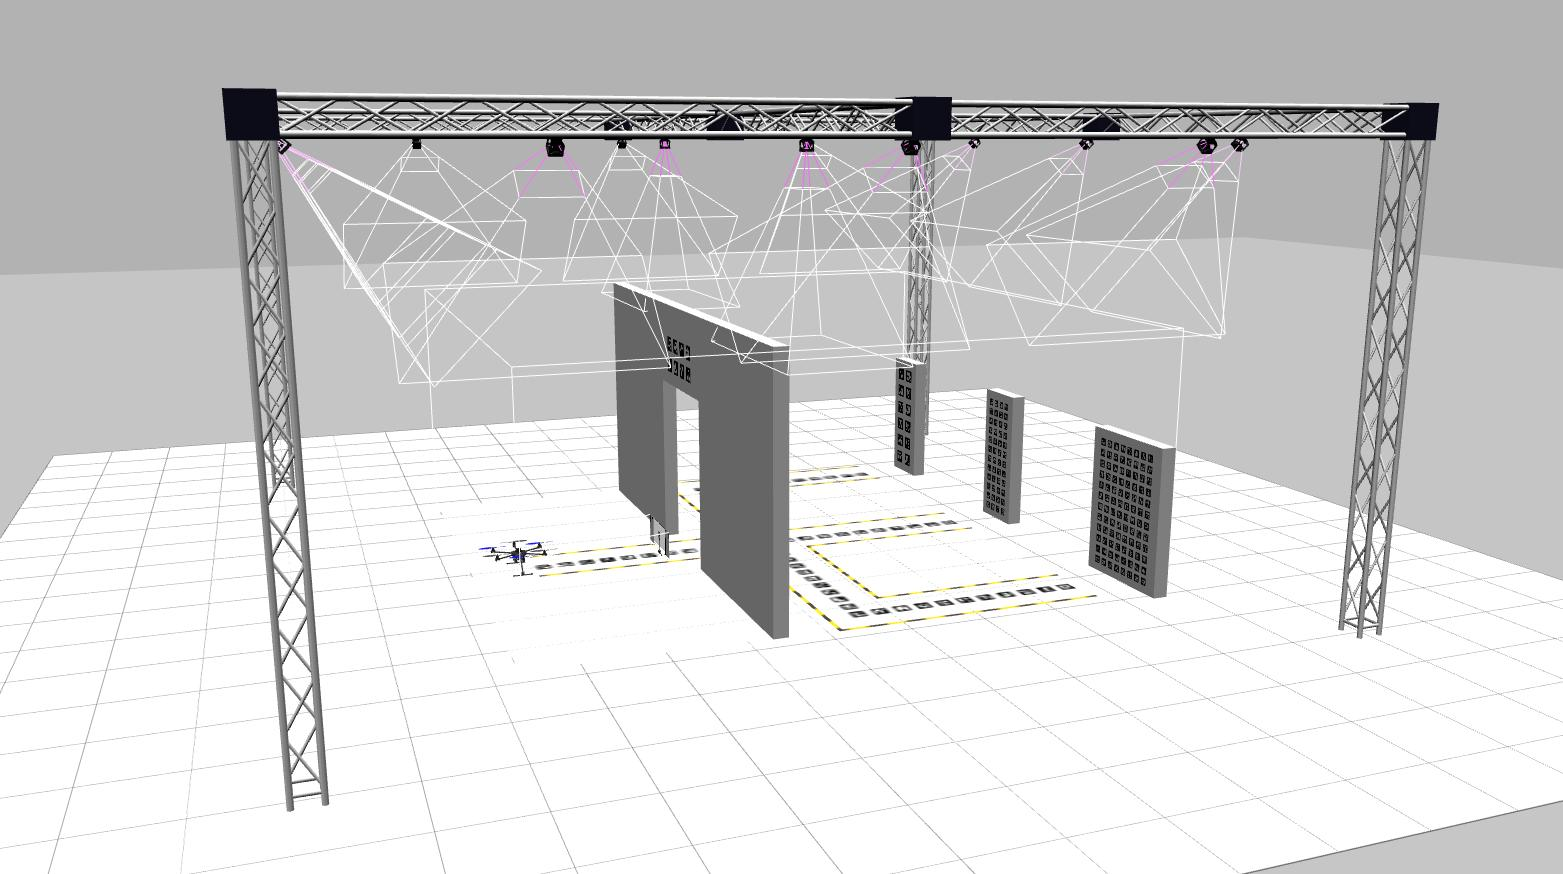
\includegraphics[width=\textwidth]{../Figures/3d-modeling/gazebo_one_pattern_view.jpg}
        \caption{}
        \label{fig:optitrack_one_pattern_aruco}
    \end{subfigure}
    \hfill
    \begin{subfigure}[t]{.48\textwidth}
        \centering
        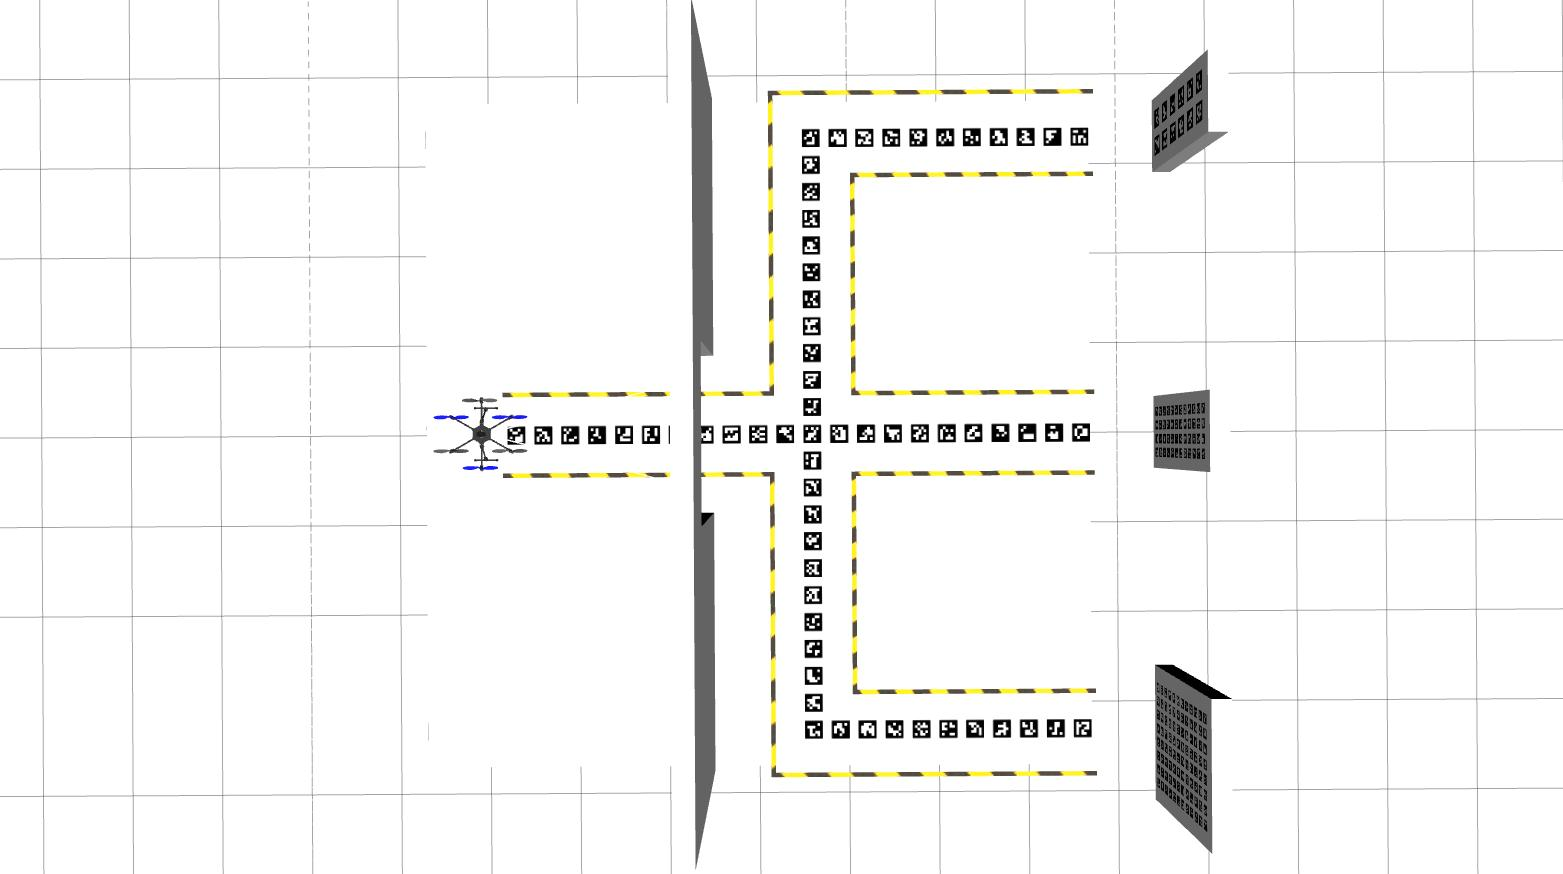
\includegraphics[width=\textwidth]{../Figures/3d-modeling/gazebo_one_pattern.jpg}
        \caption{}
        \label{fig:one_pattern_aruco}
    \end{subfigure}
    \caption{Visualization of the optitrack model in Figure \ref{fig:optitrack_one_pattern_aruco} and top view of the one pattern ArUco marker board in Figure \ref{fig:one_pattern_aruco}}
    \label{fig:one_pattern_aruco_fig}
\end{figure}


The general idea behind this design is that the UAV can fly towards the wall and locate the ArUco marker board placed at the top of the wall. This board can be seen in Figure \ref{fig:gazebo_gps2vision_board} which is called GPS2Vsion board because the UAV will use this board when switching from using GPS to vision coordinates. This will enable GPS to vision based navigation where the UAV shifts between using the GPS as the global coordinate system to that of the ArUco marker board (vision based). When the UAV has positioned itself with a certain distance away from this marker board, it will switch to using the bottom camera where the ArUco board located on the ground will function as a world coordinate system. In this scenario, the UAV is to land on one of three different locations in front of the ArUco board located at the end of each track. Here transformations of the pose of these three ArUco boards have been performed to align these with that of the ArUco board located on the ground (world coordinate) to avoid switching between different coordinate systems. This will be explained further in Section \ref{sec:pose_estimation_using_aruco_markers}. 

The ArUco markers used in these models will be ($5 \times 5$) bit markers. The GPS to vision marker board located on the top of the wall will be a ($2\times 4$) with marker length of 0.2 m and marker separation of 0.1 m, the ground marker a ($25\times25$) with marker length of 0.2 m and marker separation of 0.1 m and the landing markers ($4\times2$) with marker length of 0.2 m and marker separation of 0.1 m. These sizes have been chosen to be appropriate taking into account the size of the optitrack system where a flying height of approximately 1.5 m will be used.

If this setup were to be implemented in real life, an implementation with fewer ArUco markers would be beneficial if this would not decrease the precision of the pose estimation too much. In this small ($25\times25$) ArUco marker board scenario it would not be a general problem, but if this has to be scalable e.g. big industrial companies, great performance using a small amount of ArUco markers would be preferred.

Because the precision of the pose estimation from ArUco marker boards will be based on the number of ArUco markers located in the image \cite{DetectionOfArUcoBoards}, the estimation of the pose will be based on a full ($25\times25$) ArUco marker board and a one pattern setup as seen in Figure \ref{fig:full_pattern_aruco} and \ref{fig:one_pattern_aruco} respectively. The performance of these different setups will be evaluated in Section \ref{sec:vision_based_navigation}.  

\begin{figure}[H]
    \centering
    \begin{subfigure}[t]{.48\textwidth}
        \centering
        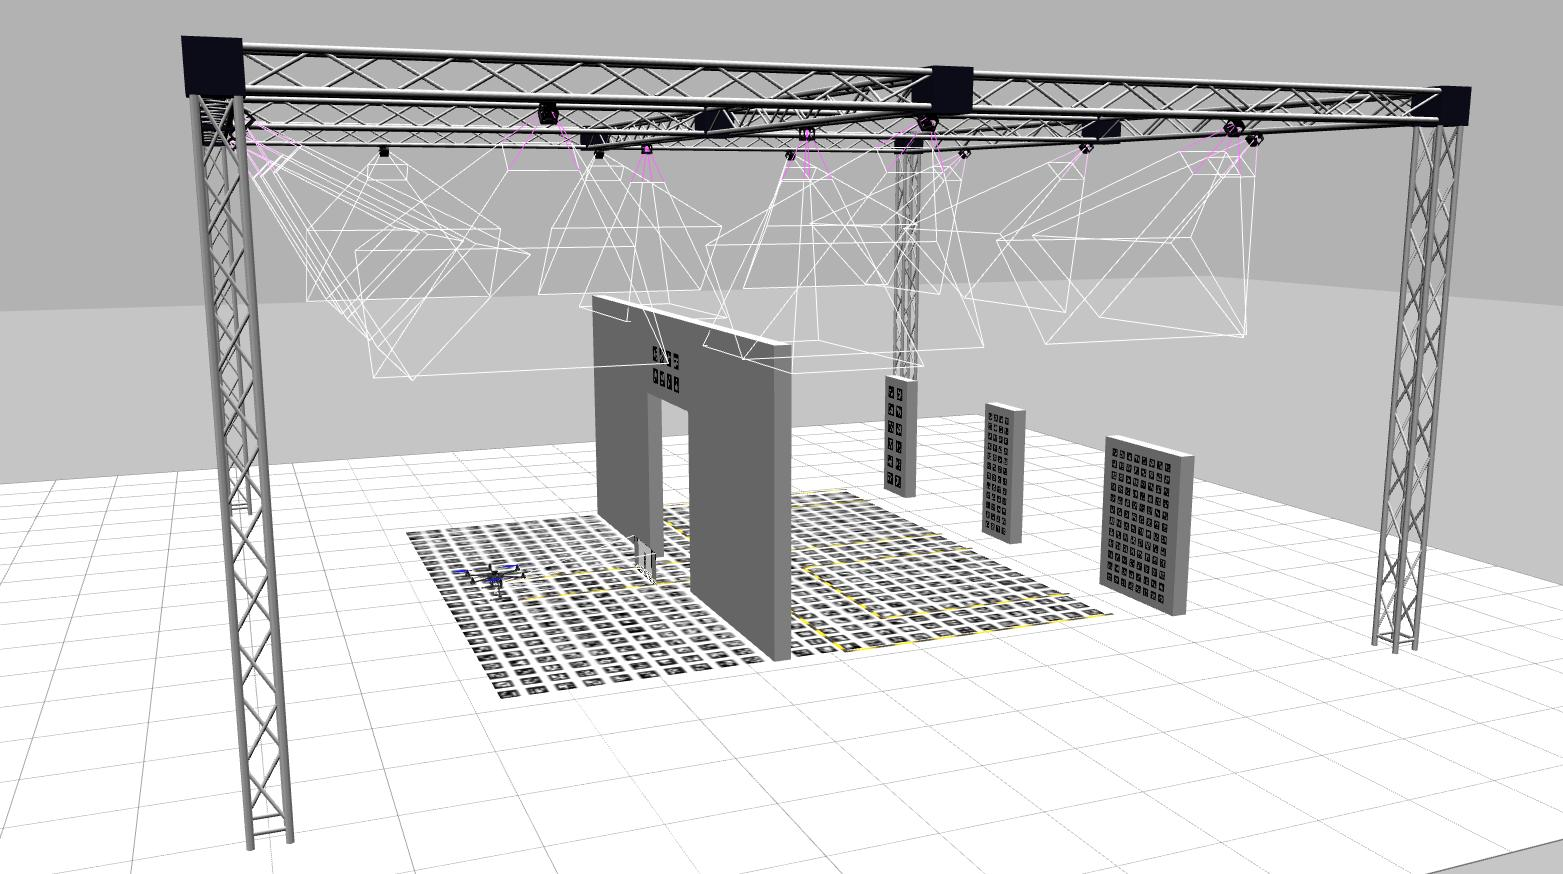
\includegraphics[width=\textwidth]{../Figures//3d-modeling/gazebo_full_pattern_view.jpg}
        \caption{}
        \label{fig:optitrack_full_pattern_aruco}
    \end{subfigure}
    \hfill
    \begin{subfigure}[t]{.48\textwidth}
        \centering
        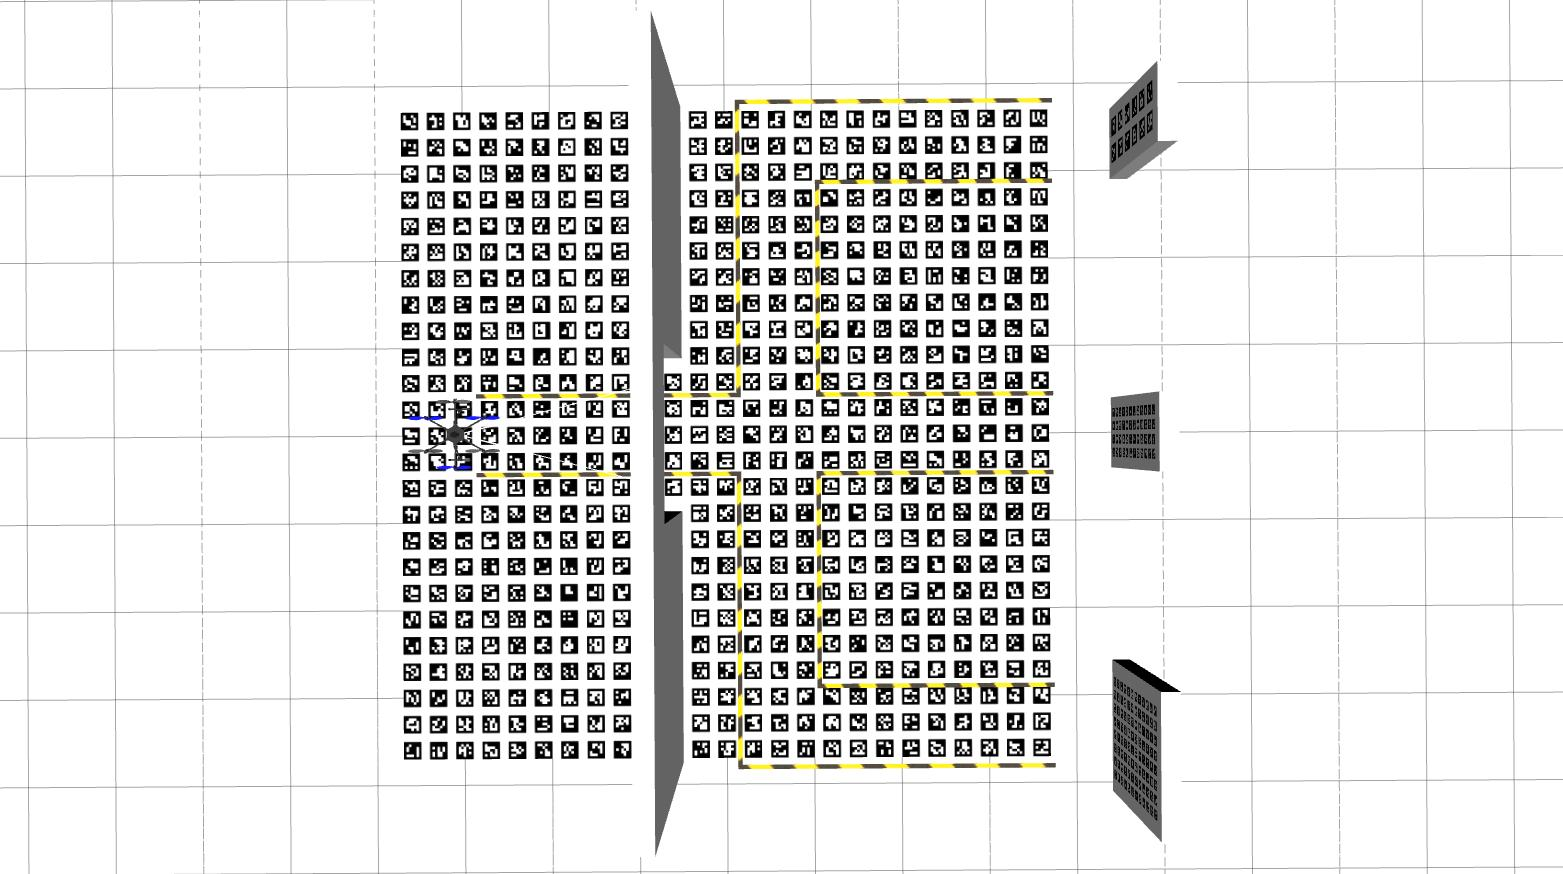
\includegraphics[width=\textwidth]{../Figures/3d-modeling/gazebo_full_pattern.jpg}
        \caption{}
        \label{fig:full_pattern_aruco}
    \end{subfigure}
    \caption{Visualisation of the optitrack model in Figure \ref{fig:optitrack_full_pattern_aruco} and top view of the full pattern ArUco marker board in Figure \ref{fig:full_pattern_aruco}}
    \label{fig:full_pattern_aruco_fig}
\end{figure}

Because relying completely on vision based navigation will put the system in a vulnerable position e.g. no markers are found in the image, optimizations have to be performed. This will be utilized through sensor fusion where the pose estimation from the ArUco marker board and sensor data from the inertial measurement unit (IMU) and barometer will be fused together to give a more reliable estimation of the current position of the drone. The implementation of this will be discussed in Section \ref{sec:sensor_fusion}. 

To evaluate the performance of sensor fusion, two models with missing ArUco markers have been created as seen in Figure \ref{fig:gazebo_one_pattern_board_missing_markers} and \ref{fig:gazebo_one_pattern_board_missing_markers_wear}. The goal of this is to have the UAV to fly a couple of meters without any global position (vision) for the pose estimation and still keep its track until the pose will be updated when markers again is visible for the UAV.

For the vision based landing, three different ArUco marker boards have been created. These can be seen in Figure \ref{fig:gazebo_landing_board_one}, \ref{fig:gazebo_landing_board_two} and \ref{fig:gazebo_landing_board_three} which are called landing board one, landing board two and landing board three respectively. Because these boards have been created is to analyze the performance of pose estimation when a different number of ArUco markers are visible in the image. More ArUco markers in the image should give better pose estimates, because more points from each marker are fused together to give a better pose estimation. Hence, these three landing boards will be used to analyze if a very high number of ArUco markers in the image are required for a precise landing. Results of this can be seen in Section \ref{sec:hold_pose_using_aruco_pose_estimation} and \ref{sec:vision_based_landing}. 

\begin{figure}[H]
    \centering
    \begin{subfigure}[t]{.22\textwidth}
        \centering
        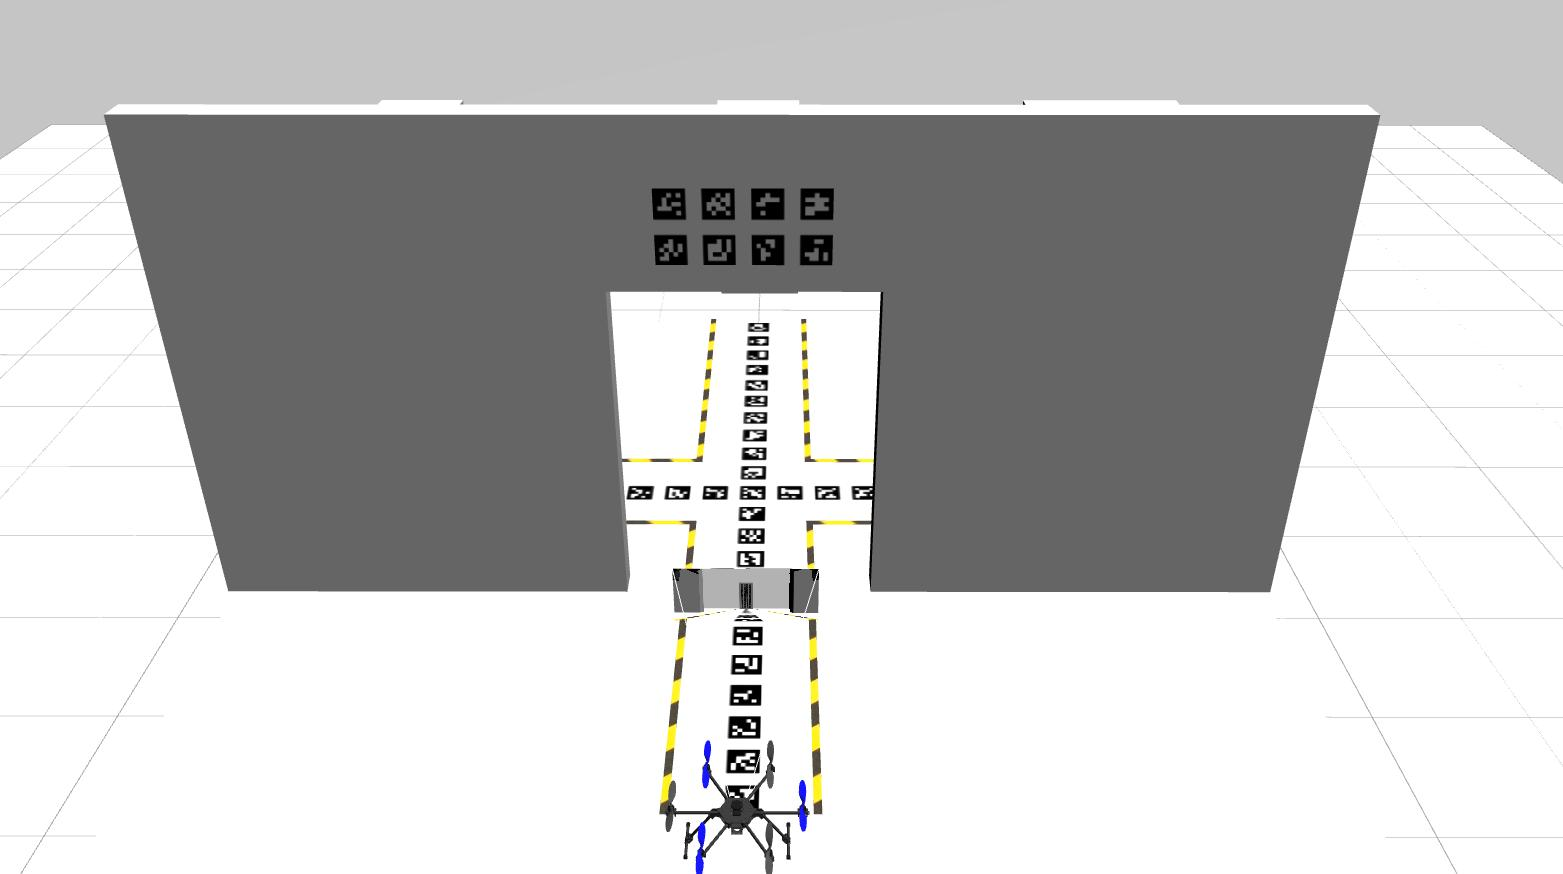
\includegraphics[width=\textwidth]{../Figures/3d-modeling/gazebo_gps2vision_board.jpg}
        \caption{}
        \label{fig:gazebo_gps2vision_board}
    \end{subfigure}
     \hspace{0.2em}
    \begin{subfigure}[t]{.22\textwidth}
        \centering
        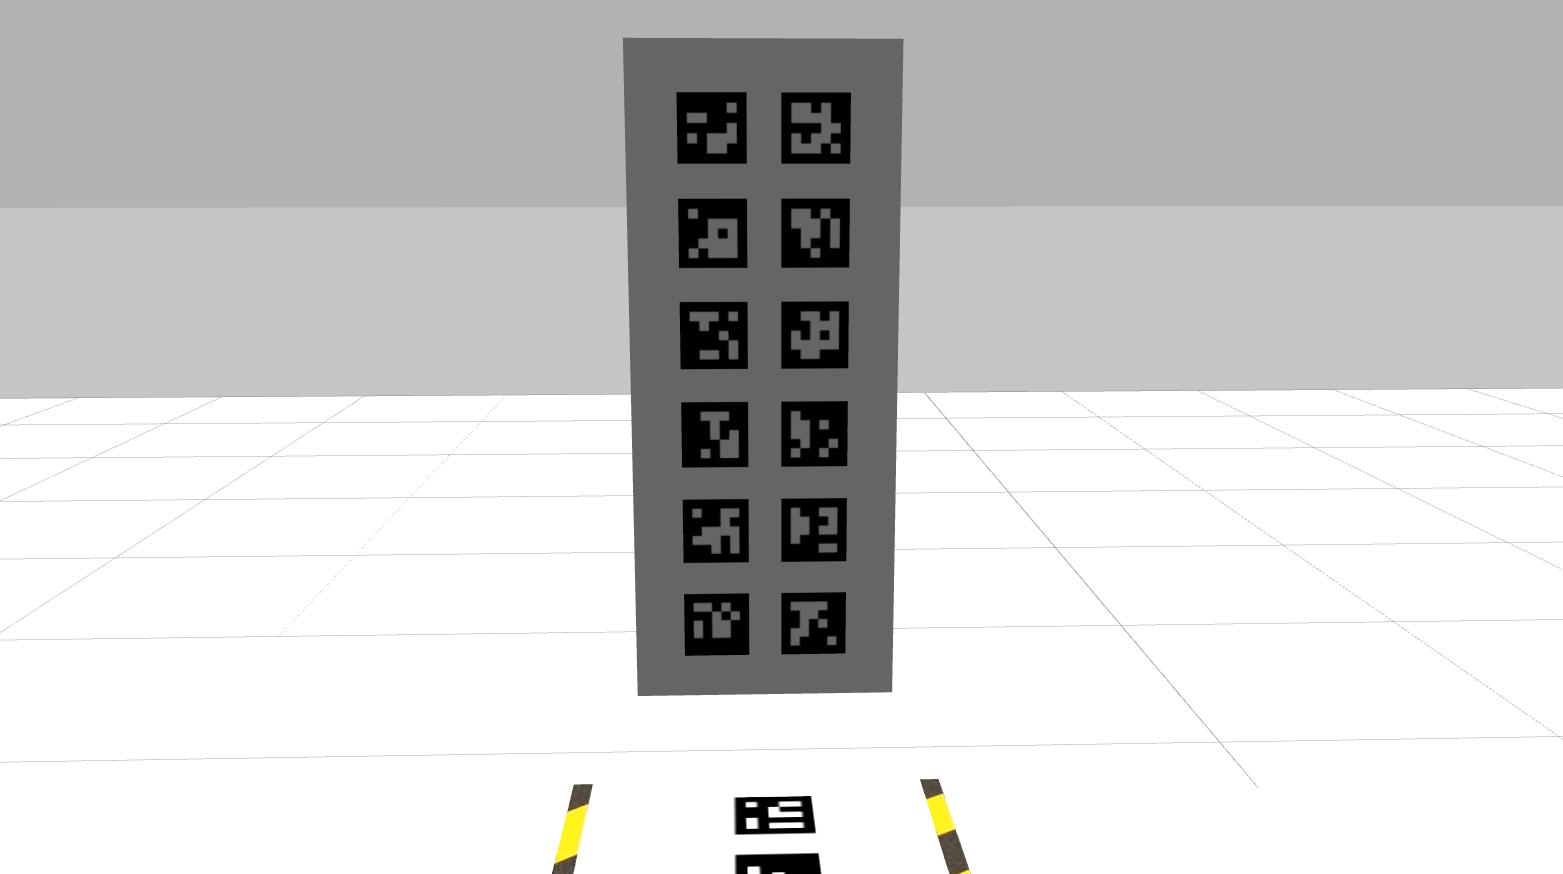
\includegraphics[width=\textwidth]{../Figures/3d-modeling/gazebo_landing_board_one.jpg}
        \caption{}
        \label{fig:gazebo_landing_board_one}
    \end{subfigure}
     \hspace{0.2em}
    \begin{subfigure}[t]{.22\textwidth}
        \centering
        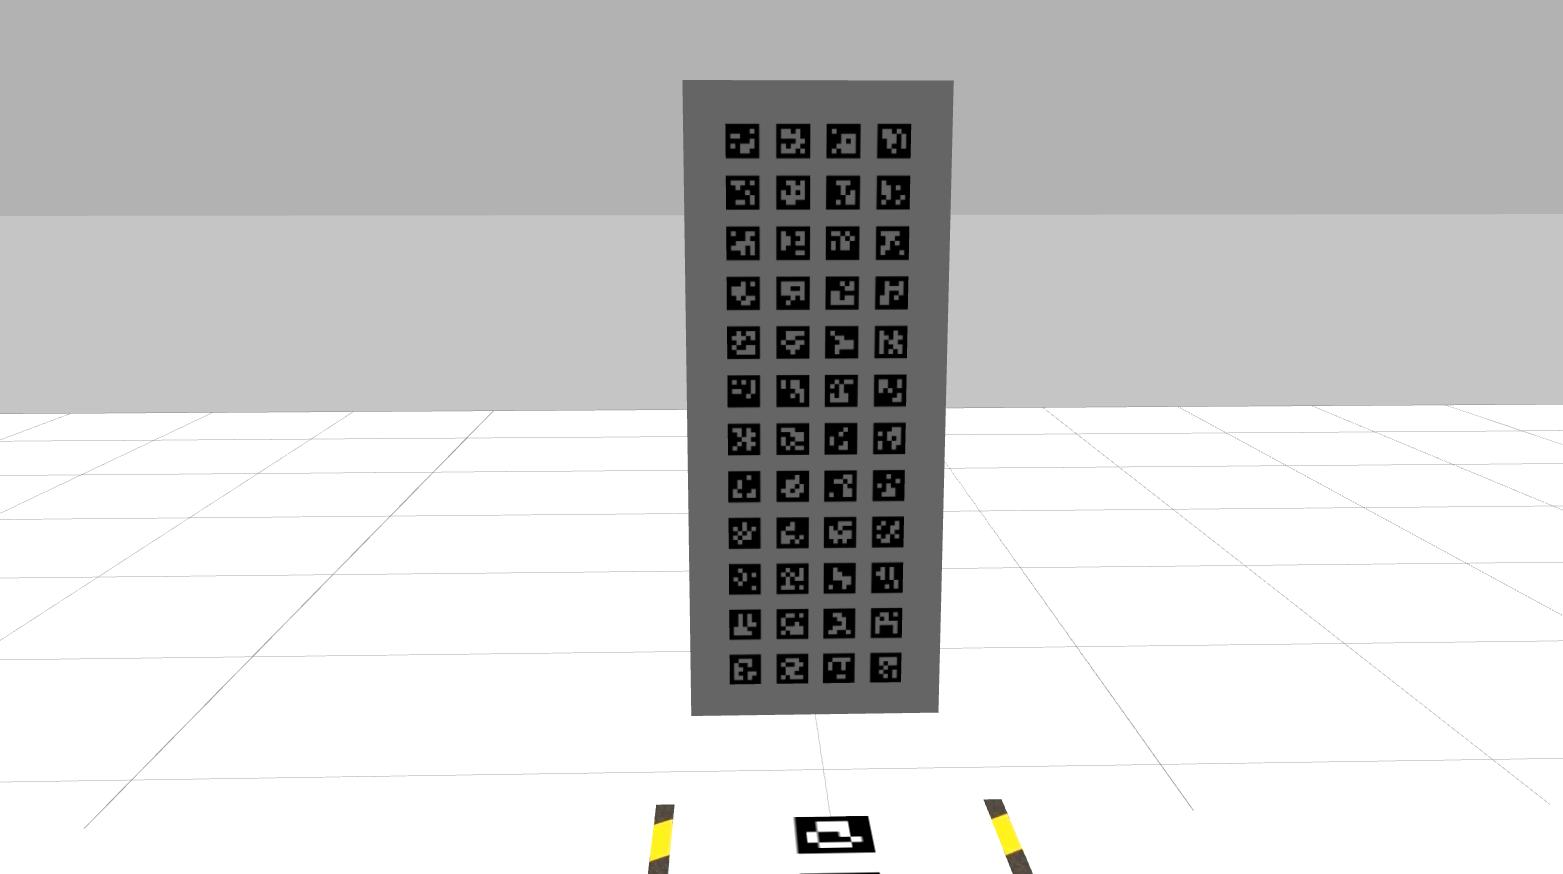
\includegraphics[width=\textwidth]{../Figures/3d-modeling/gazebo_landing_board_two.jpg}
        \caption{}
        \label{fig:gazebo_landing_board_two}
    \end{subfigure}
         \hspace{0.2em}
    \begin{subfigure}[t]{.22\textwidth}
        \centering
        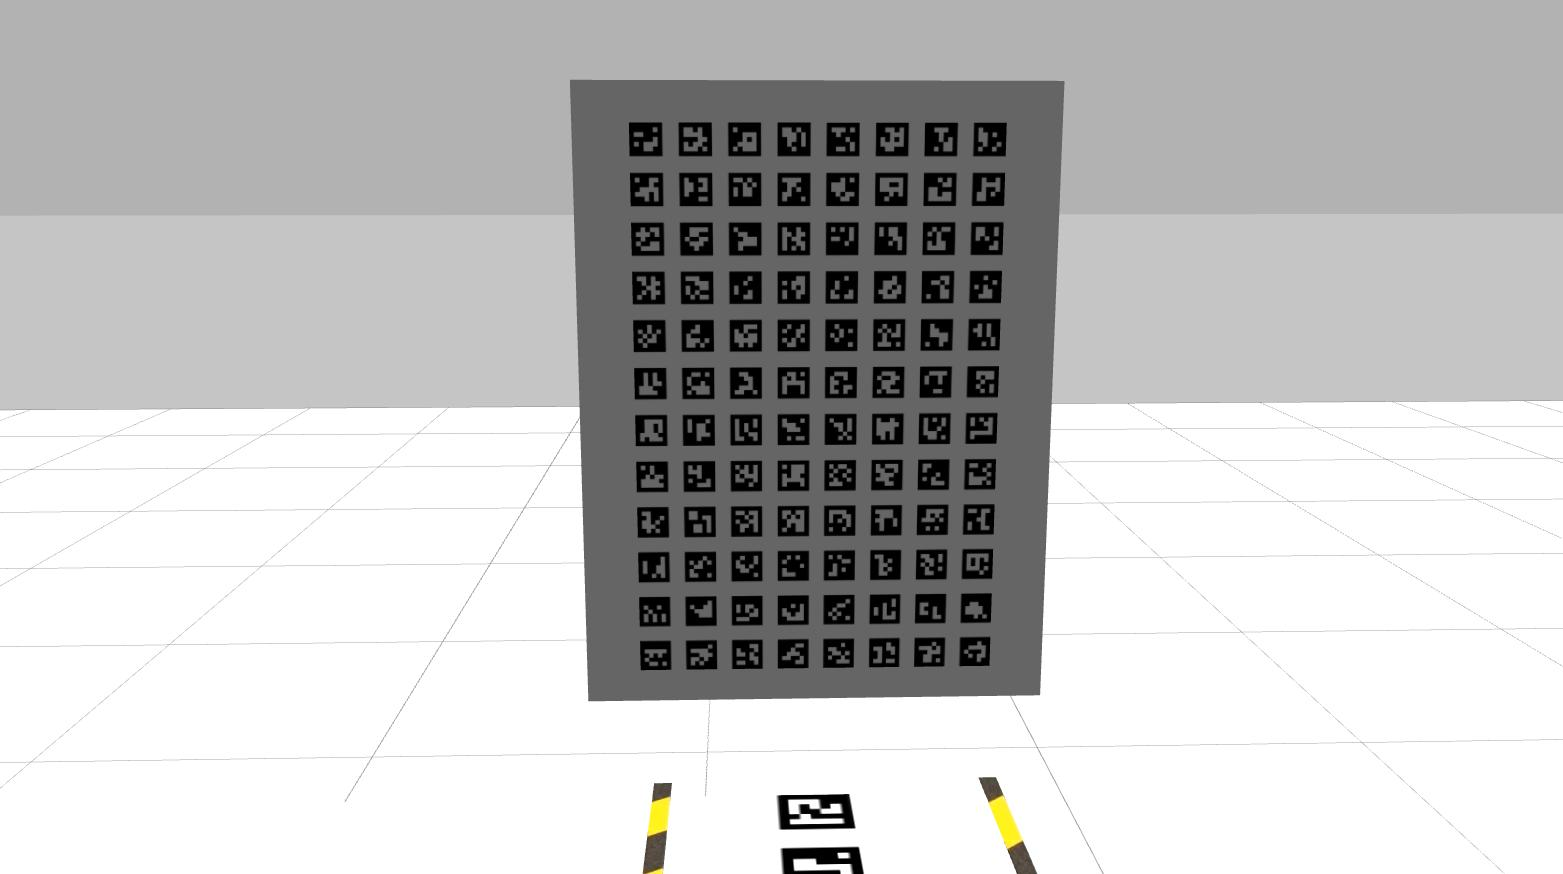
\includegraphics[width=\textwidth]{../Figures/3d-modeling/gazebo_landing_board_three.jpg}
        \caption{}
        \label{fig:gazebo_landing_board_three}
    \end{subfigure}
    \caption{Illustration of the created ArUco marker boards used in simulation. The board in \ref{fig:gazebo_gps2vision_board} is used for the GPS to vision transition for navigation and the boards in Figure \ref{fig:gazebo_landing_board_one}, \ref{fig:gazebo_landing_board_two} and \ref{fig:gazebo_landing_board_three} are used for vision based landing}  
    \label{fig:gazebo_aruco_marker_boards}
\end{figure}      

\begin{figure}[H]
    \centering
    \begin{subfigure}[t]{.20\textwidth}
        \centering
        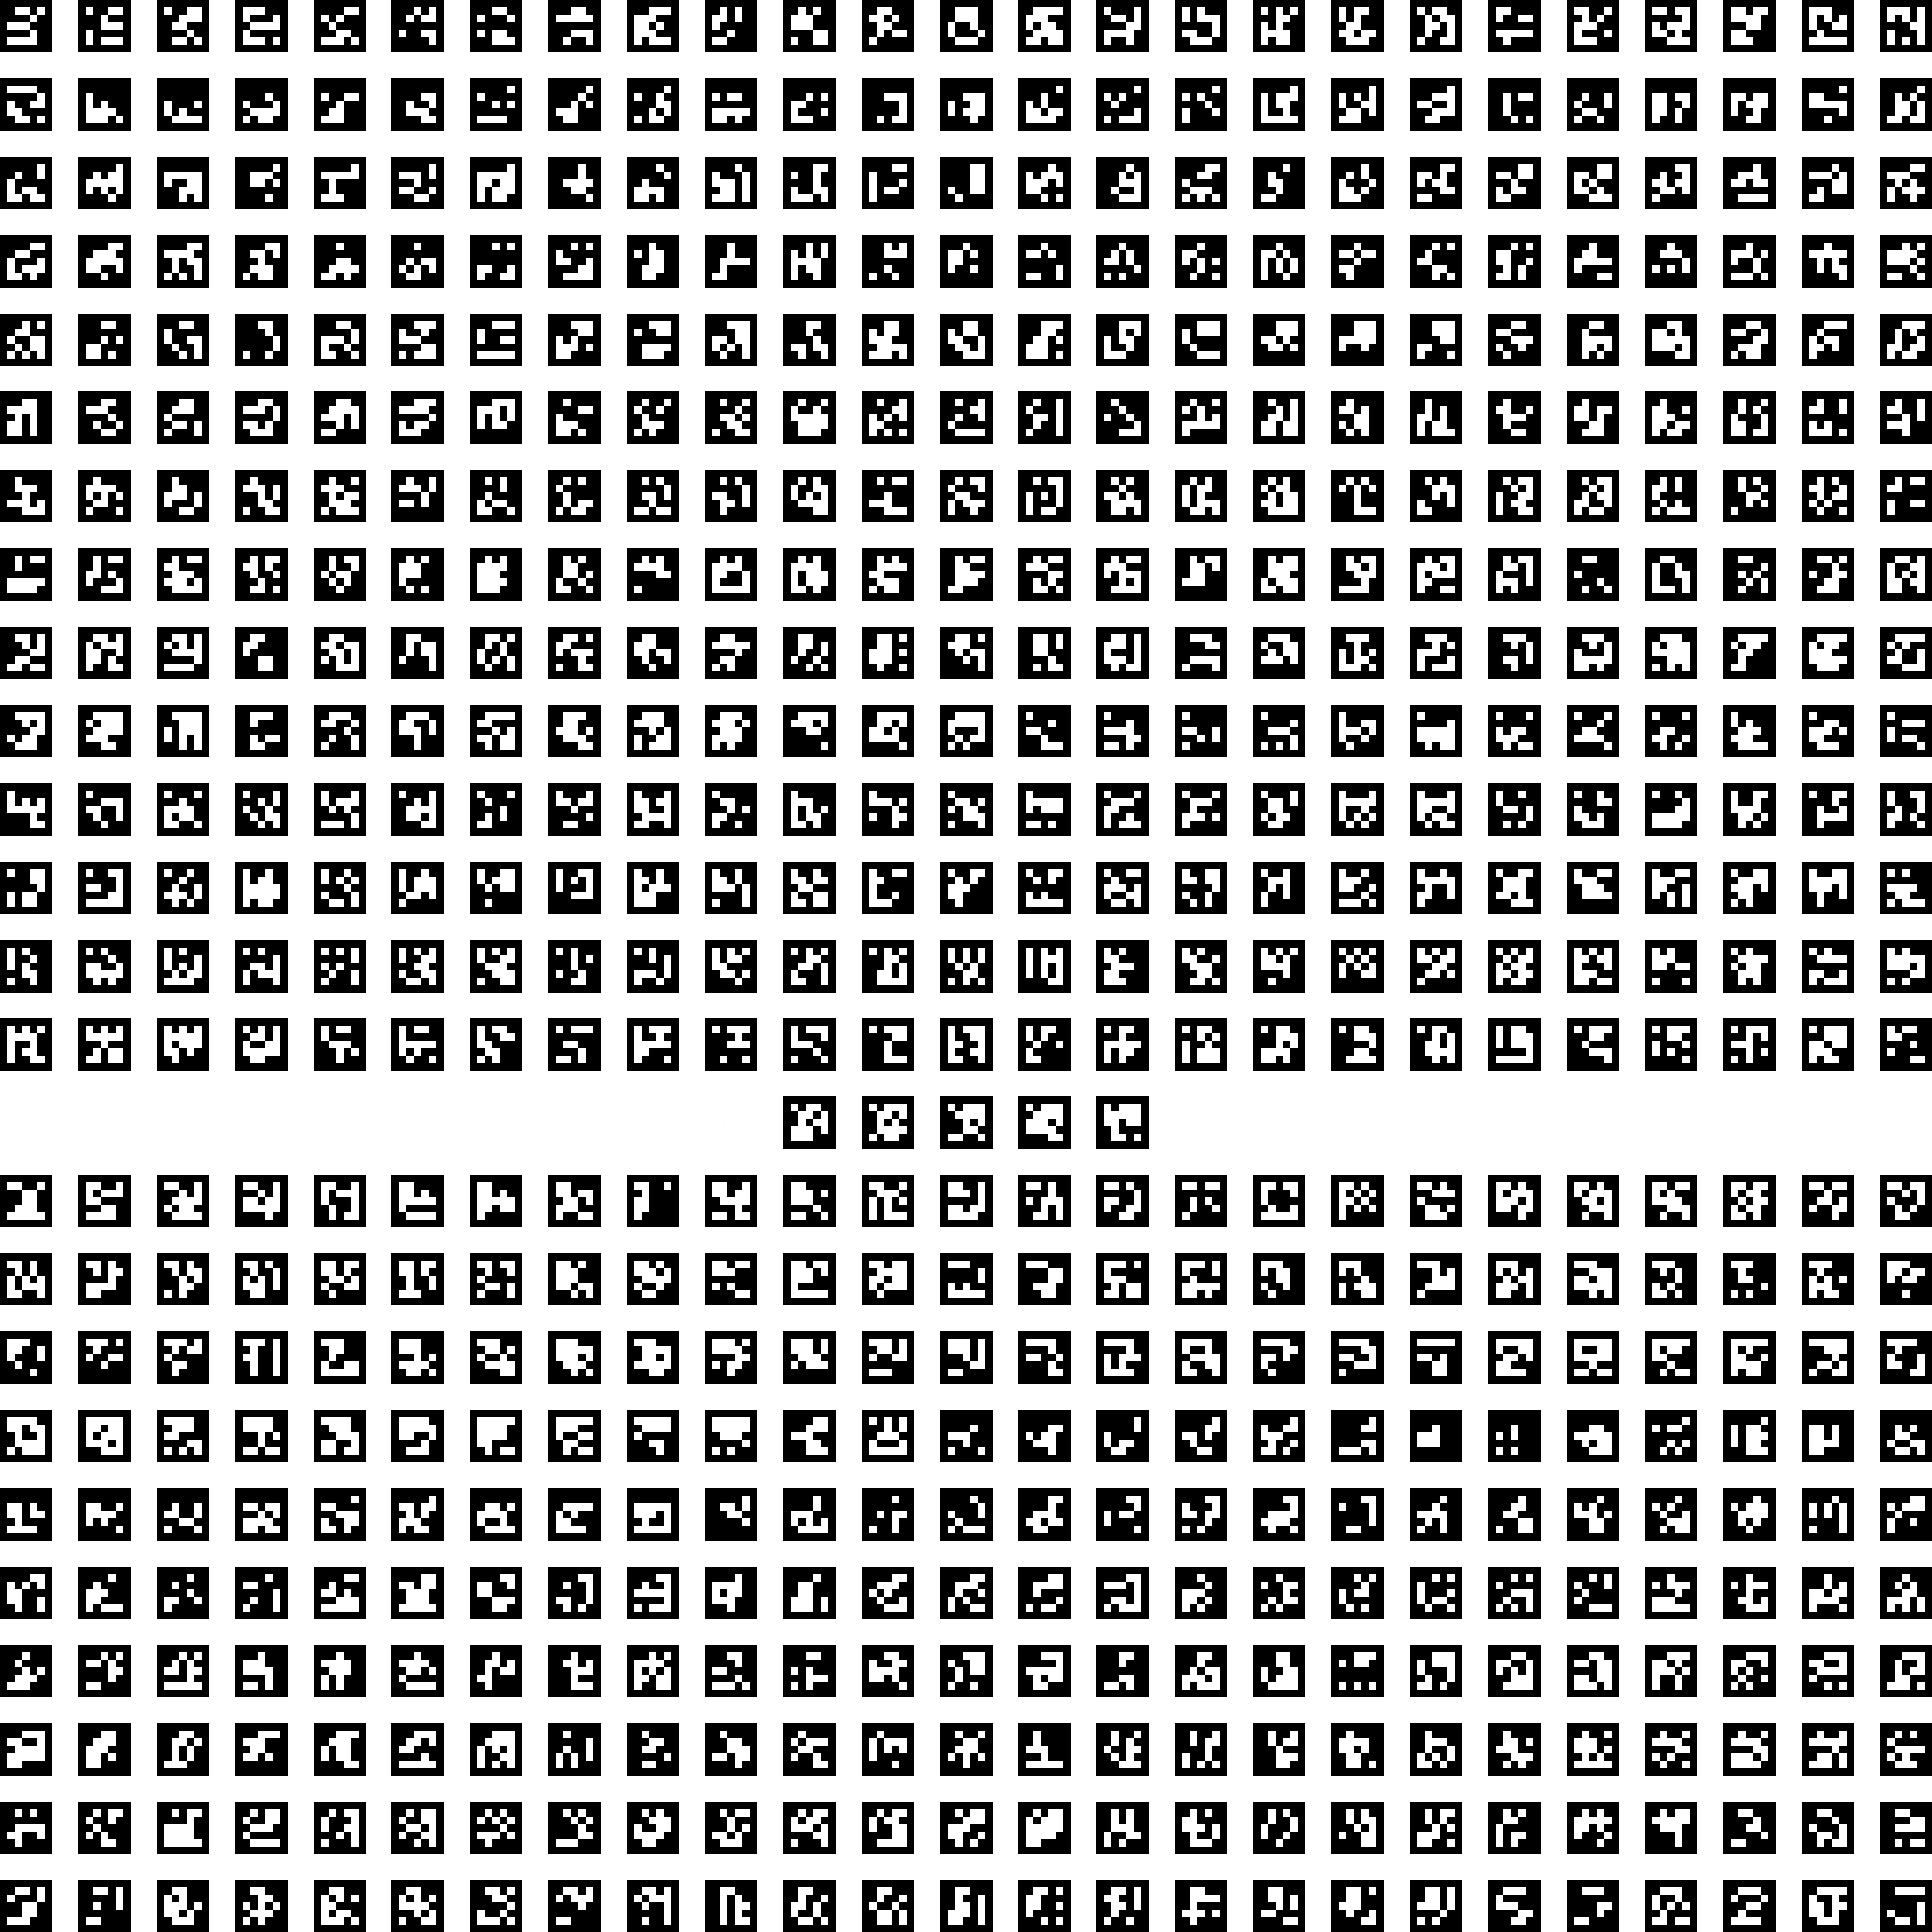
\includegraphics[width=\textwidth]{../Figures/vision_navigation/grid_board_new_200_full.png}
        \caption{}
        \label{fig:gazebo_full_pattern_board}
    \end{subfigure}
     \hspace{0.2em}
    \begin{subfigure}[t]{.20\textwidth}
        \centering
        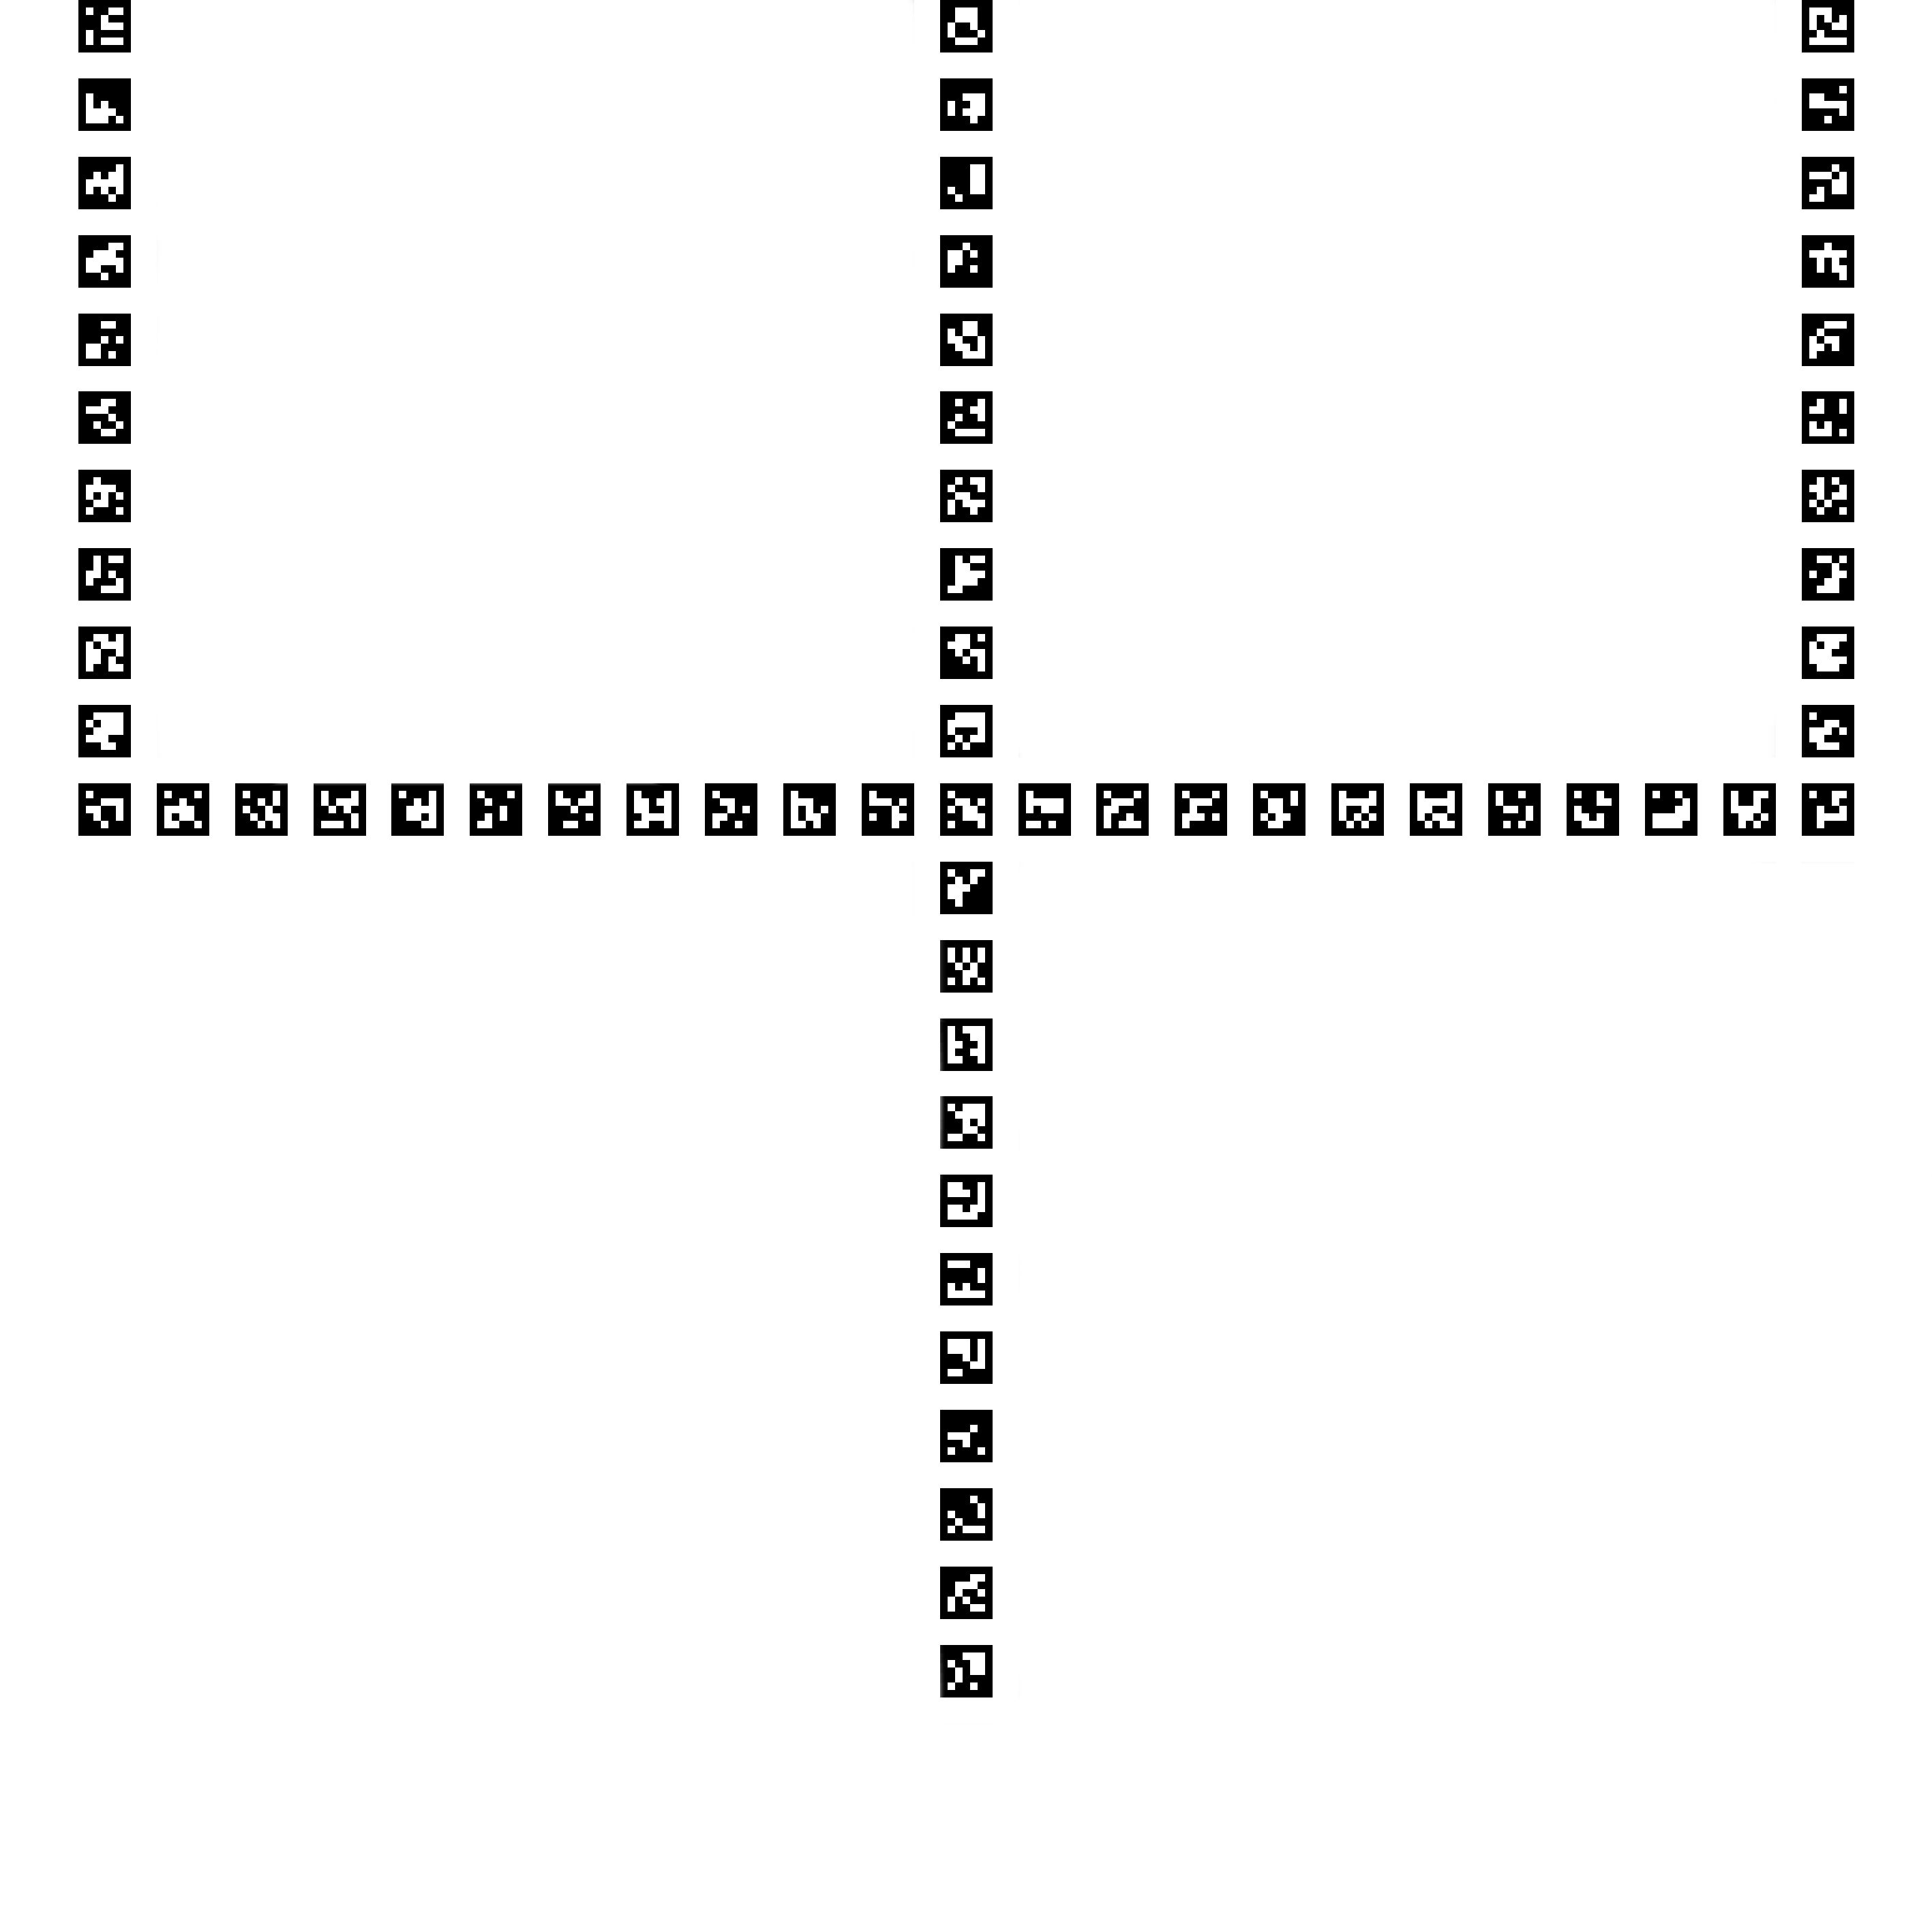
\includegraphics[width=\textwidth]{../Figures/vision_navigation/grid_board_new_200_big_onepattern.png}
        \caption{}
        \label{fig:gazebo_one_pattern_board}
    \end{subfigure}
     \hspace{0.2em}
    \begin{subfigure}[t]{.20\textwidth}
        \centering
        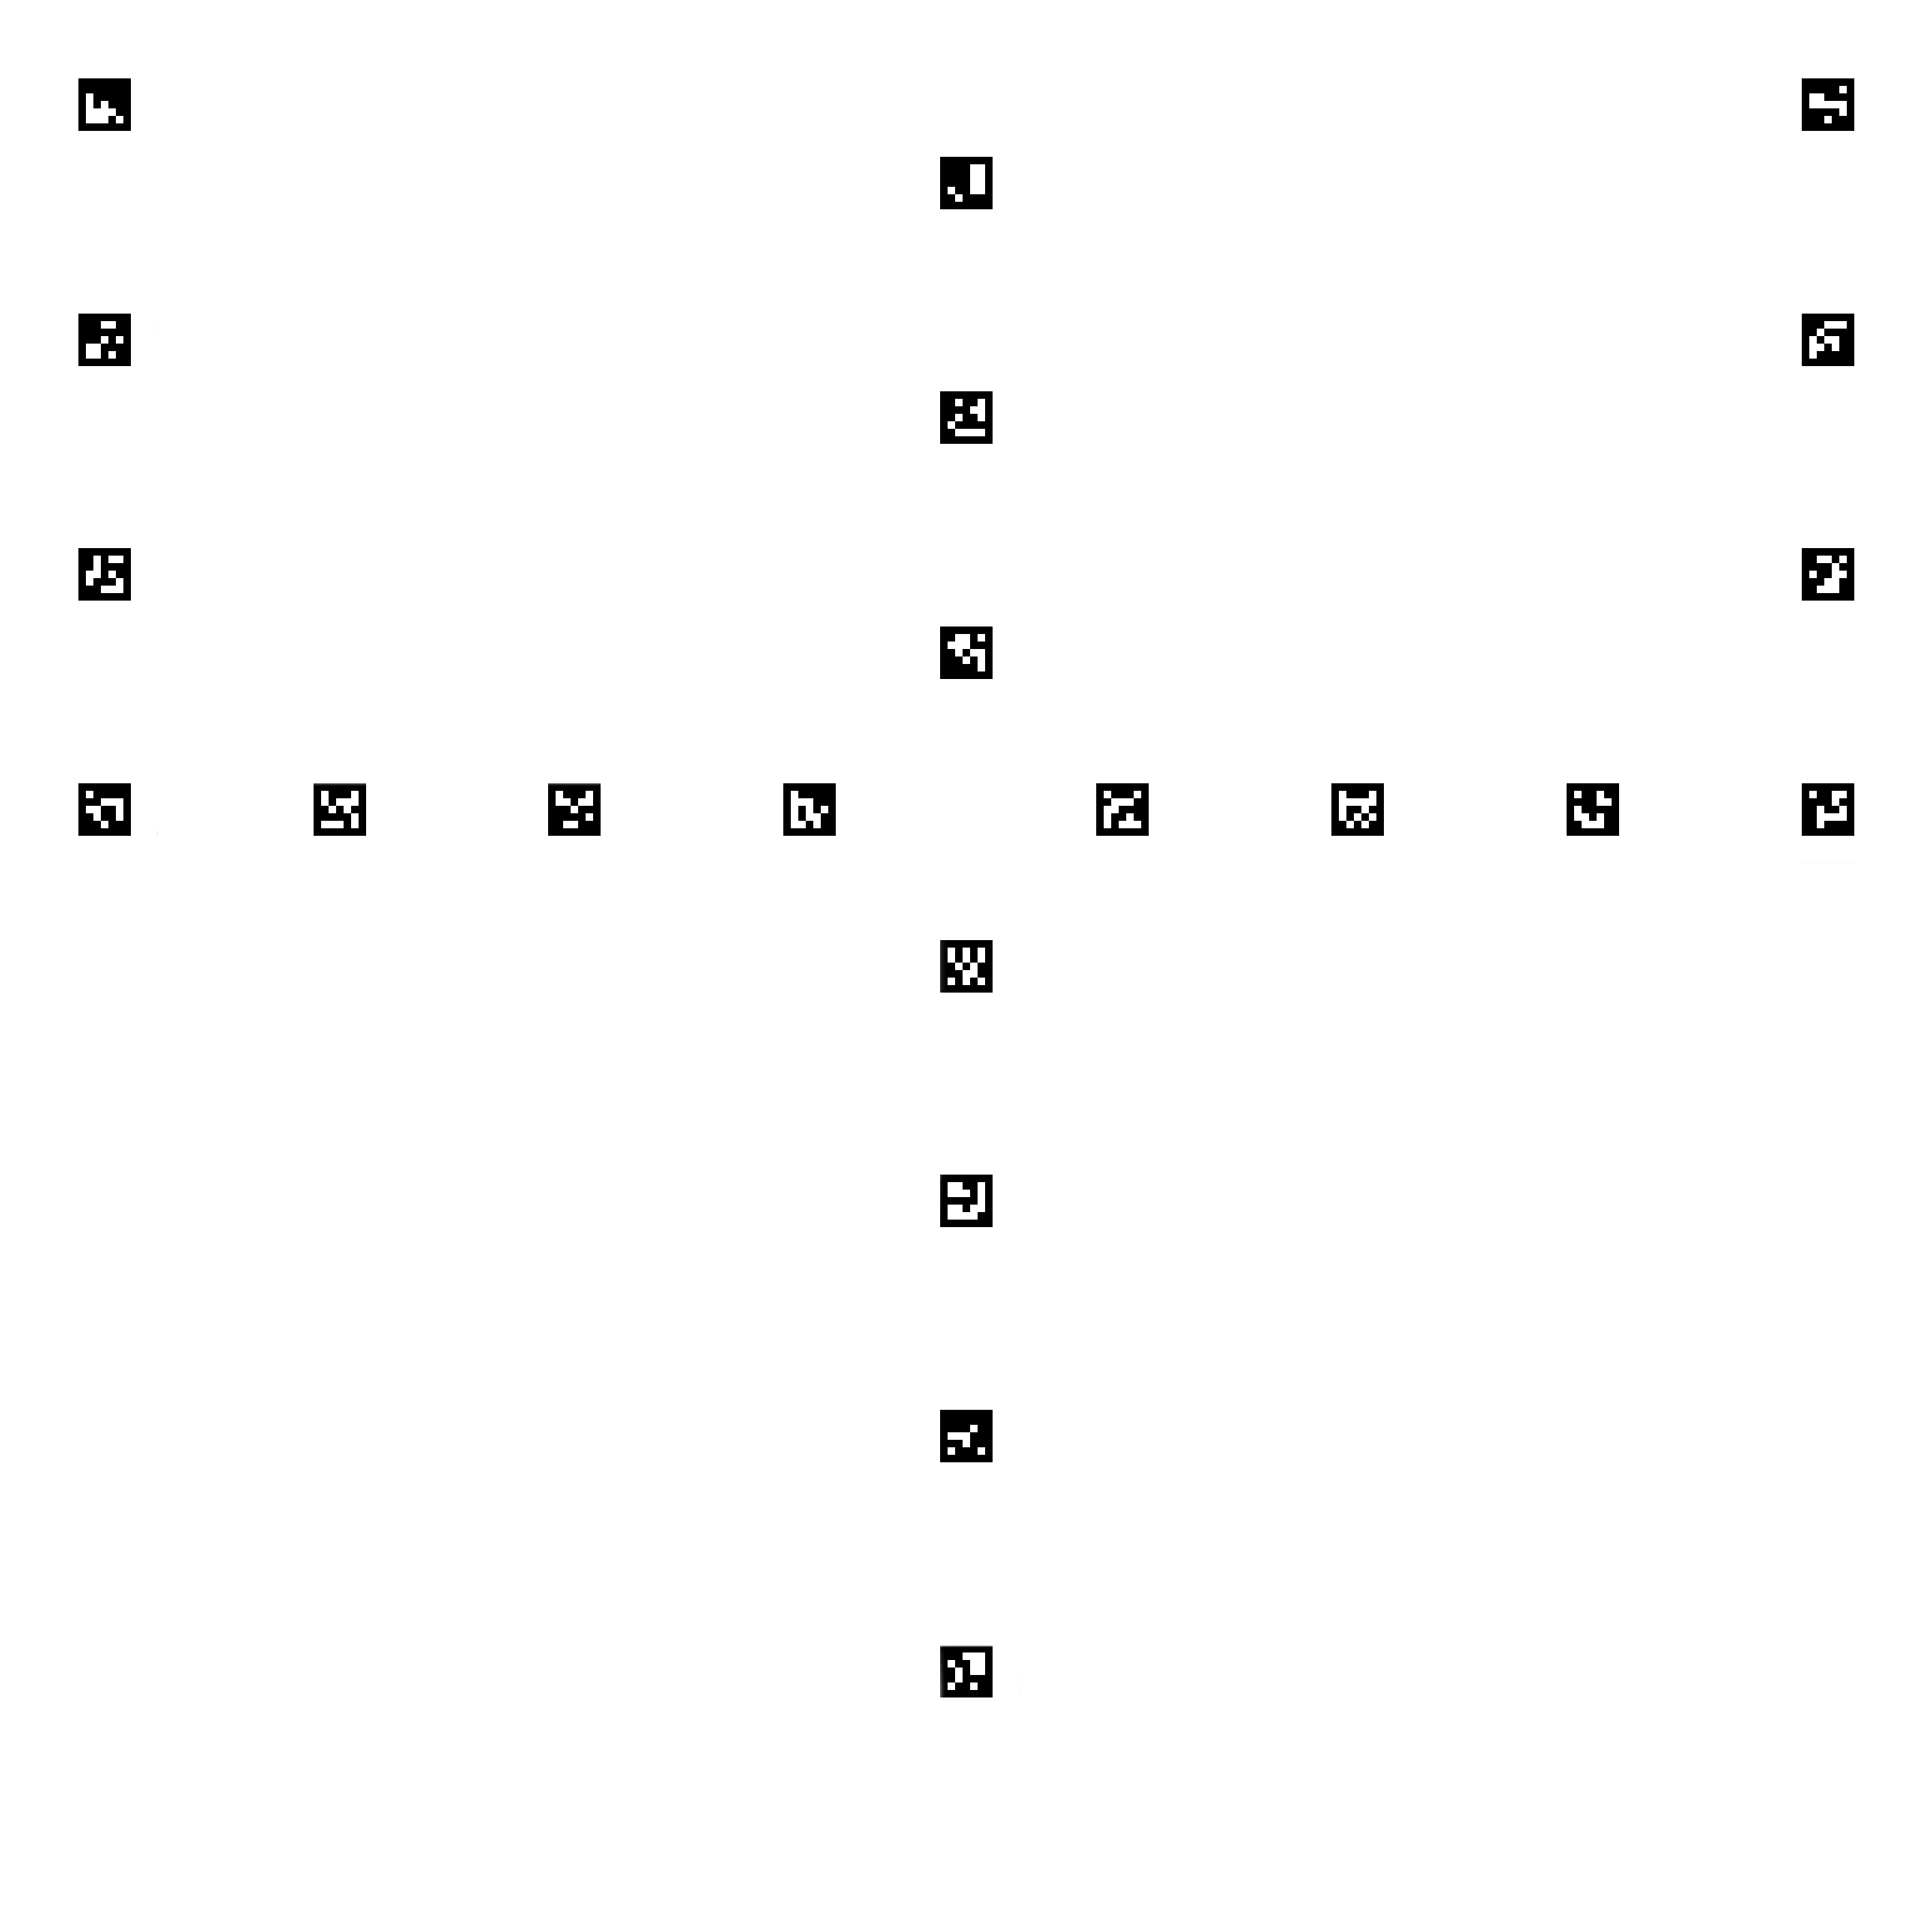
\includegraphics[width=\textwidth]{../Figures/vision_navigation/grid_board_new_200_big_onepattern_missing_markers1.png}
        \caption{}
        \label{fig:gazebo_one_pattern_board_missing_markers}
    \end{subfigure}
         \hspace{0.2em}
    \begin{subfigure}[t]{.20\textwidth}
        \centering
        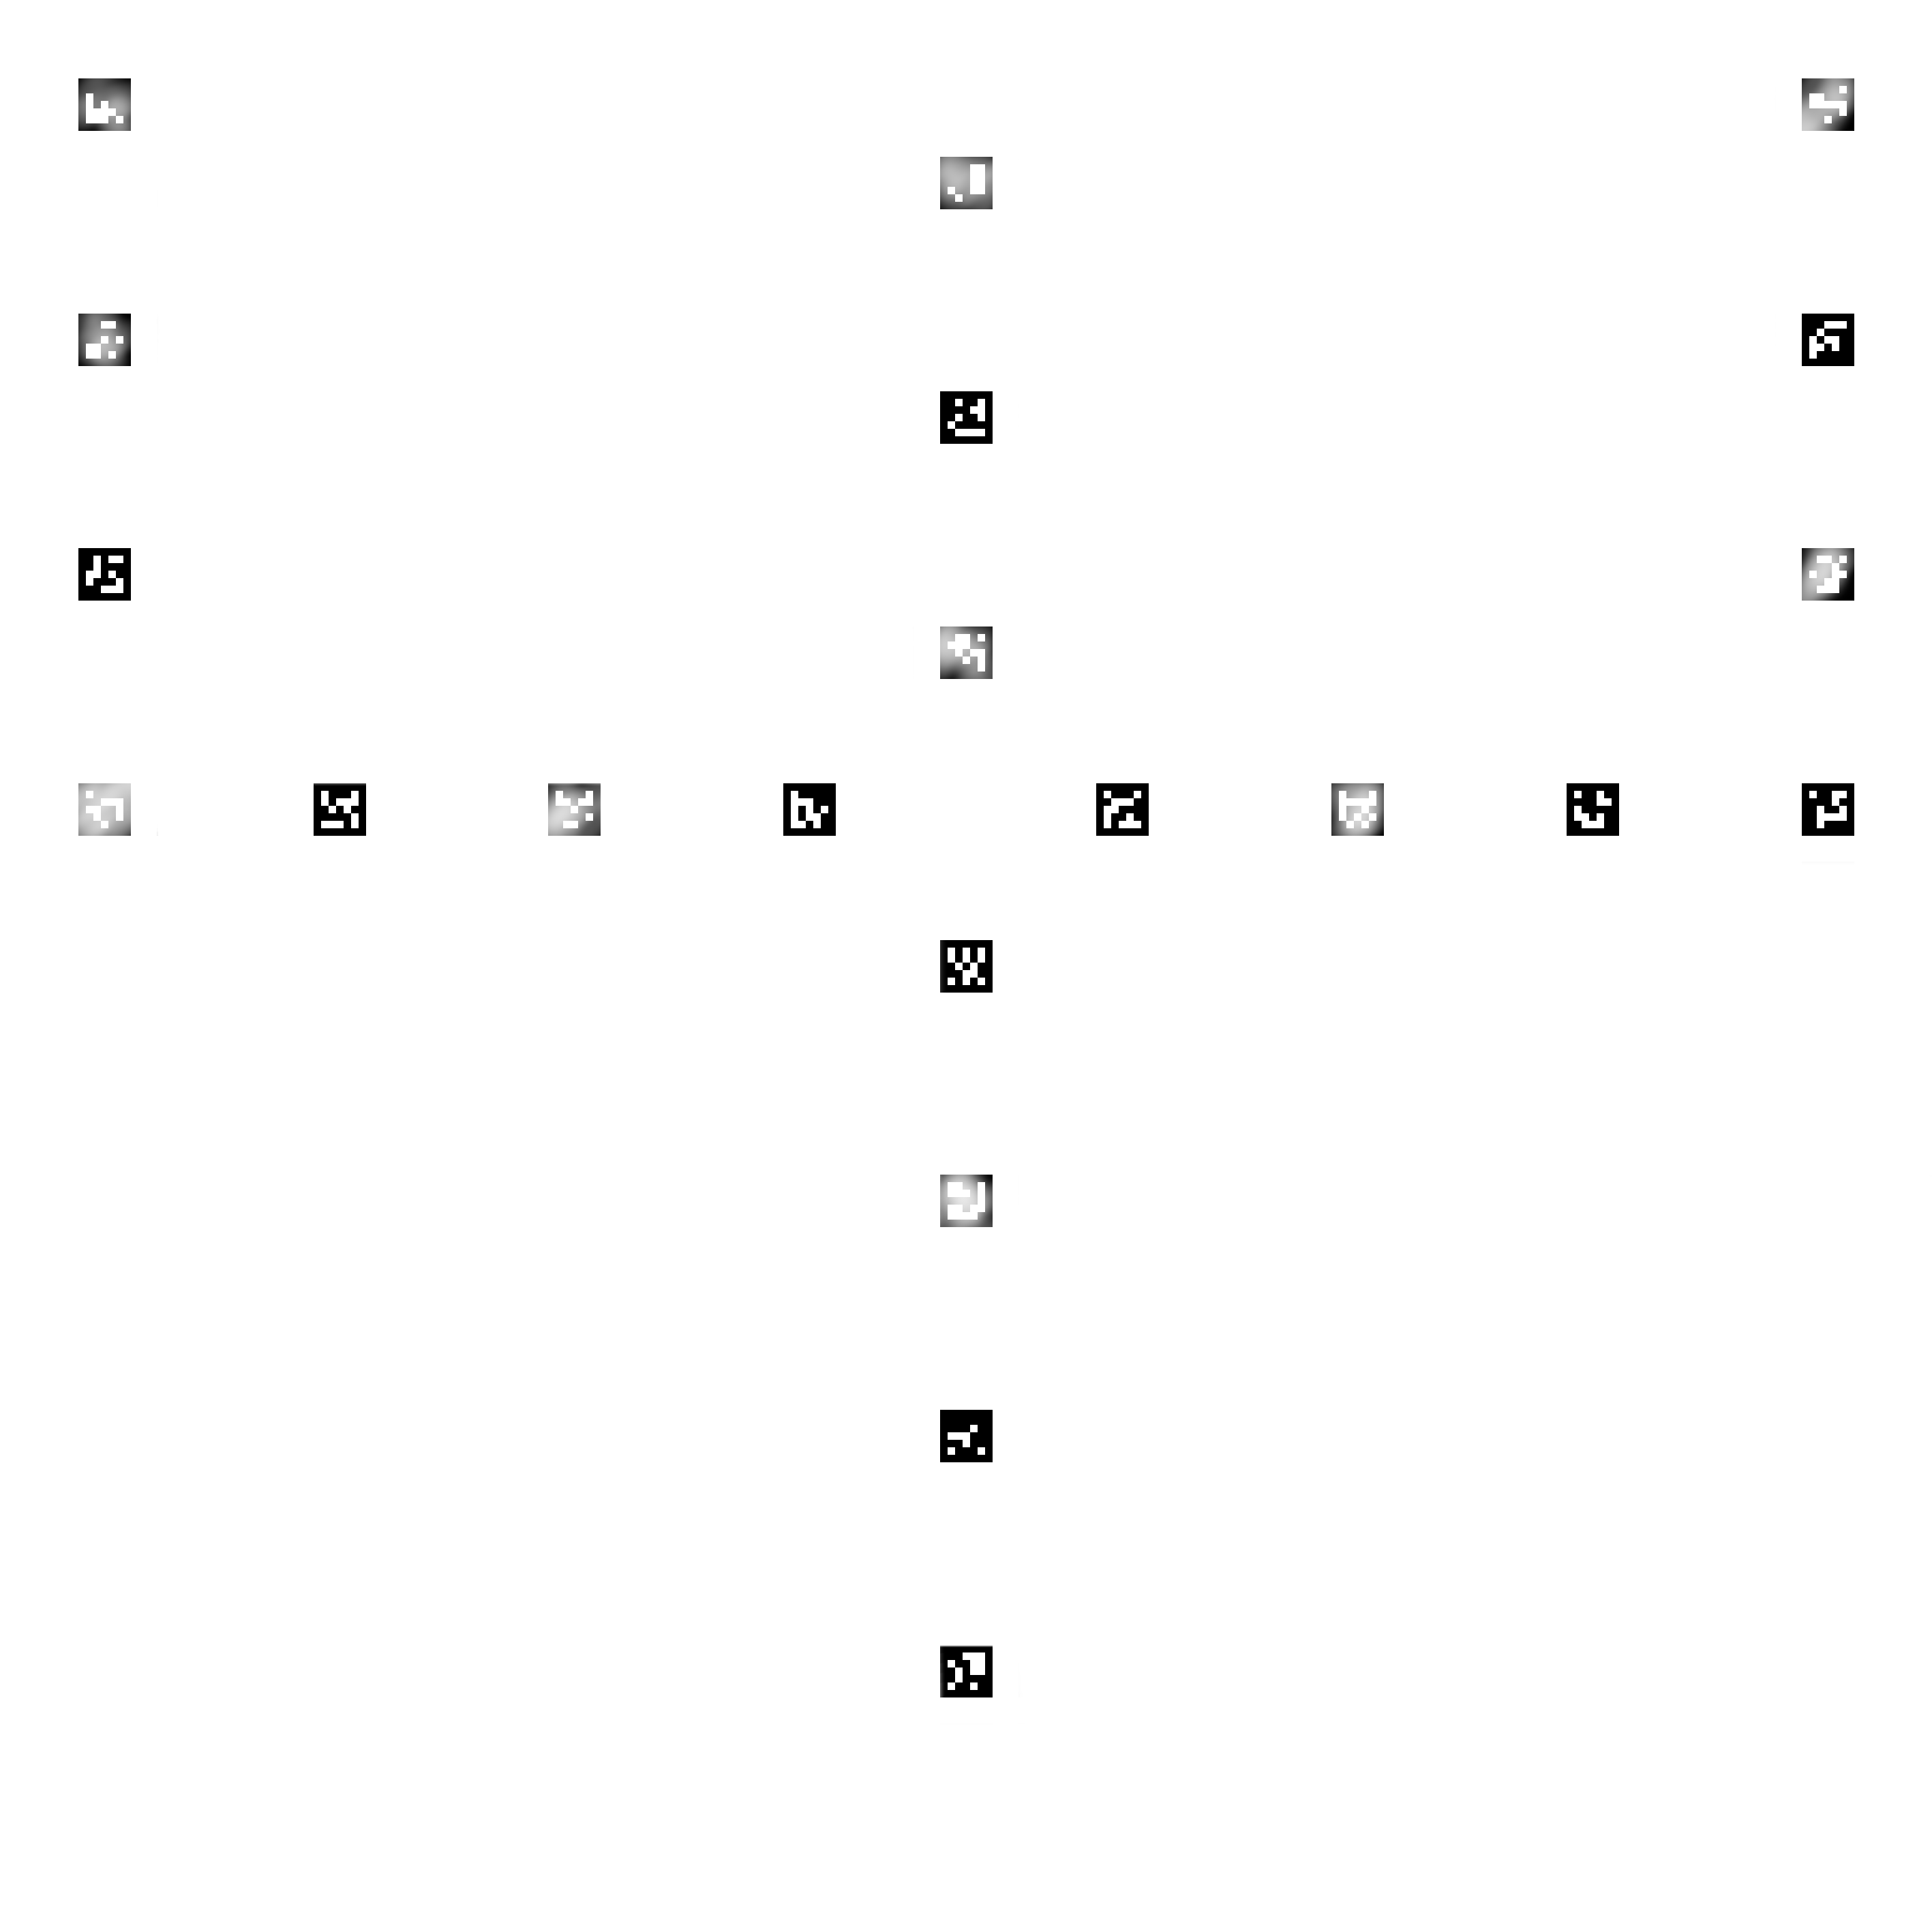
\includegraphics[width=\textwidth]{../Figures/vision_navigation/grid_board_new_200_big_onepattern_missing_markers_wear.png}
        \caption{}
        \label{fig:gazebo_one_pattern_board_missing_markers_wear}
    \end{subfigure}
    \caption{Illustration of the ArUco marker boards used which are located on the ground. Four \textbf{.world} files will be created where each include one of the following boards namely the full board in Figure \ref{fig:gazebo_full_pattern_board}, the one pattern board in Figure \ref{fig:gazebo_one_pattern_board} and the one pattern board with missing markers and custom made wear in Figure \ref{fig:gazebo_one_pattern_board_missing_markers} and \ref{fig:gazebo_one_pattern_board_missing_markers_wear} respectively}  
    \label{fig:gazebo_full_and_one_patterns_boards}
\end{figure}

\subsubsection{Gazebo simulator}
\label{sec:gazebo}

Gazebo is an open source 3D robotic simulator which integrates the open dynamics engine (ODE) physics engine, openGL rendering and supports code for both actuator control and sensor simulation. Using this software, the UAV can be tested and simulated in environments and conditions close to real life. Hence, all tests will be performed in simulation before further action will be executed with the UAV. Furthermore, wind can be applied to the simulation which will also be a critical aspect to consider before deployment of the UAV. 

To use the newly created models, a world file must be defined. The world file includes all elements which are to be included in a given simulation such as robots, lights, sensors, objects etc. The file must end with a \textit{.world} extension to be recognized as a world file. The GZServer will read this file which builds the world as a virtual environment for which the robot can operate. This means that the operation can be visualized using GZClient or be run in the background only using GZServer to save systems resources. The latter corresponds to running Gazebo in headless mode, which is a great feature to use if a number of simulations have to be performed in a automatic fashion.

The world file uses the SDF format which contains things like \textit{worlds}, \textit{models} etc. Joints can be set to be either revolute or prismatic according to the wanted configuration. To each joint a link can be attached. The collision, visualization and inertia tags specifies the visualization for the model, collision detection and physics in Gazebo respectively. The static tags are used for models which have to be static throughout a simulation like ground, tress etc. The same SDF format is used when creating a model, where the \textit{.dae} file is included to use the 3D models created in Blender.  

The plugins in gazebo are code which is compiled as a shared library and inserted into the simulation. These plugins includes world, model, sensors, system, visual and GUI. For instance, if one wants to include a feature to an existing model, like a wind plugin, these can be included into the world file to be used in a simulation. This wind plugin will be used in some of the simulations for stress testing of the ArUco pose estimation and the flight control in general.

\subsection{Autonomous flight}

This section deals with the implementation of autonomous flight of the UAV. The PX4 autopilot will be used as flight controller which offers many features to enable autonomous flight. This is discussed in Section \ref{sec:px4_flight_stack}. Along the PX4 software, robot operating system (ROS) will be used which enables onboard computing on the Raspberry Pi and transmission of messages to the PX4 using the MAVROS package. ROS is discussed in Section \ref{sec:offboard_control}. For easy setup and access to the drone QGroundControl is used which is discussed in Section \ref{sec:qgroundcontrol}. 

The main reason for chosen PX4, ROS and QGroundControl is because the software have been widely used in MSc in Engineering in robot systems with
specialization in unmanned aerial systems technology at the University of Southern Denmark. A lot of experience have been gained which will be utilized in the implementation of autonomous flight.

\subsubsection{QGroundControl}
\label{sec:qgroundcontrol}

\href{https://docs.qgroundcontrol.com/master/en/}{QGroundControl} offers full flight control and setup of the vehicles for a number of flight controllers including PX4. The advantage of using this as the GCS is that one gets immediate updates of the state of the drone e.g pose, power of battery, errors etc. to a laptop using a wireless connection.  Moreover, the latest stable PX4 Firmware can be fetched and flashed directly to the SD card of the PX4. An visualization of the QGroundcontrol GUI can be seen in Figure \ref{fig:qgroundcontrol}.

The primary usage of this software will be to change parameters on the drone in flight e.g vertical and horizontal velocities, changes of parameters of PIDs for pose control etc. Furthermore, sensor calibration of the compass, gyroscope and accelerometer can easily be done before every flight to achieve the best performance of the drone. Besides of this, transmitter and telemetry setup can be performed where different flight modes can be encoded to belong to a giving channel on the transmitter for manual control of the drone. Especially two flight modes will be encoded in the system to be triggered when the transmitter is used namely \textit{\textbf{altitude}} and \textit{\textbf{manual}}. The \textit{\textbf{altitude}} mode offers altitude control where the altitude is keep constant using the barometer in the PX4 sensors. In \textit{\textbf{manual mode}}, the pilot has full control of the drone where he has to control both altitude and attitude of the drone. These modes can then be used to take manual control of the drone if something unexpected should happen when the drone is in autonomous offboard mode. A more thorough description of the different flight modes offered in PX4 can be seen in \href{https://docs.px4.io/v1.9.0/en/flight_modes/}{flight modes}.

\begin{figure}[H]
    \centering
    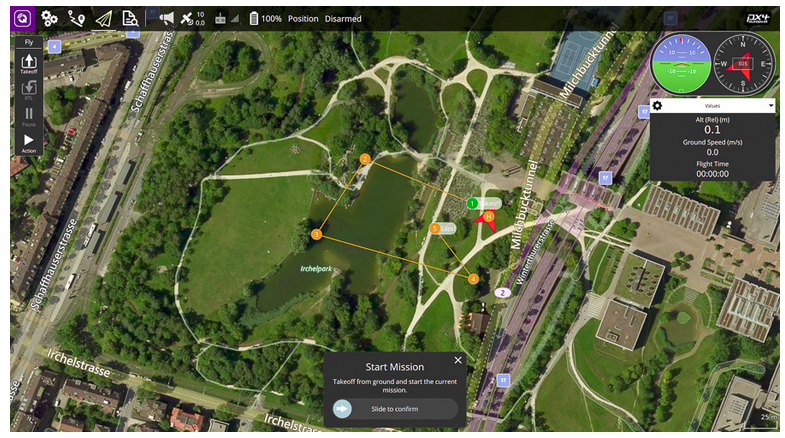
\includegraphics[width=0.7\linewidth]{../Figures/qgroundcontrol.png}
    \caption{Illustrations of the GUI in QGroundControl. Waypoints can be placed that the drone can be set to follow from the yellow circles. Here the orientation of the drone can be seen illustrated by the red arrow. The drone may also be controlled giving commands e.g takeoff}
    \label{fig:qgroundcontrol}
\end{figure}

\begin{figure}[H]
    \centering
    \begin{subfigure}[b]{.27\textwidth}
        \centering
        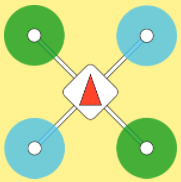
\includegraphics[height=4.0cm]{../Figures/Quadrotor.png}
           %\vspace{0.5em}
        \caption{Quadrotor airframe}
        \label{fig:quadrotor}
    \end{subfigure}
    %\hspace{-2.8em}
    \begin{subfigure}[b]{.27\textwidth}
        \centering
        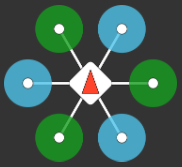
\includegraphics[height=4.0cm]{../Figures/hexarotor.png}
        \caption{Hexarotor airframe}
        \label{fig:hexarotor}
    \end{subfigure}
    \begin{subfigure}[b]{.34\textwidth}
        \centering
        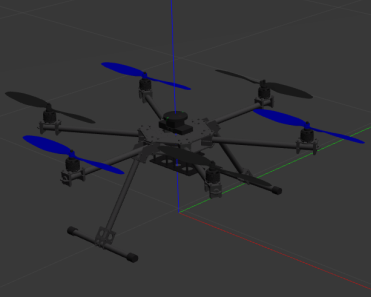
\includegraphics[height=4.0cm]{../Figures/sdu_drone.png}
        \caption{SDU drone model}
        \label{fig:sdu_drone}
    \end{subfigure}
    \caption{Illustration of different air frame configurations which can be set in QGroundControl. The Holybro QAV250 Quadcopter uses the configuration in Figure \ref{fig:quadrotor} and the SDU drone model seen in Figure \ref{fig:sdu_drone} developed by \href{https://portal.findresearcher.sdu.dk/da/persons/jes-grydholdt-jepsen}{Jes Grydholdt Jepsen} uses the configuration seen in Figure \ref{fig:hexarotor}}
    \label{fig:airframes}
\end{figure}

Two different air frames were considered to be used. These can be seen in Figure \ref{fig:quadrotor} and \ref{fig:hexarotor}. The reason for having two different setups is because of the current Covid-19 situation where access to Hans Christian Andersen airport in Odense is limited. If possible, the SDU drone model seen in Figure \ref{fig:sdu_drone}, will be used in real life for testing at the airport. Otherwise, the Holybro QAV250 Quadcopter will be used. The reason for wanting to fly with the SDU drone is because of the gained experience in the Expert in teams project (EiT) 2020, where this drone was used throughout the project. That is also why the SDU drone model will be used in the simulations. 

When configuring air frames in QGroundControl, a number predefined setups can be used. This goes for the Holybro QAV250 Quadcopter and SDU drone where all parameters are predefined like PID parameters for pose and attitude control.

As it may be noticed in Figure \ref{fig:quadrotor} and \ref{fig:hexarotor}, the green and blue colors illustrate the spin direction of the propellers. Blue is counterclockwise and green clockwise. The use of QGroundControl offers the possibility to check the spin direction of each propeller separately to insure a proper setup. This feature will also be used in this case for safety reasons.  

 
\subsubsection{Offboard control}
\label{sec:offboard_control}

For the implementation of offboard control as well as communication between units, ROS will be used. ROS is an open source software framework to be used in robot applications. This includes a number of libraries and tools with the aim of simplifying the creation of new robotic solutions. Another important feature is the message handling between nodes in the ROS architecture which is visualized in Figure \ref{fig:ros}. Here the ROS master keeps track on all the nodes in the system an each node goes through registration via the master. Then each node can publish or subscribe to messages which is initiated through the master. This is called topics under the ROS framework and will be used in offboard control where a number of nodes have to communicate to each other.

\begin{figure}[H]
    \centering
    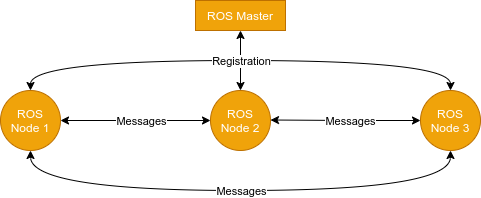
\includegraphics[width=0.75\linewidth]{../Figures/ros.png}
    \caption{Illustration of a high level view of the architecture in the communication between nodes in ROS. Here three ROS nodes have been created, but the number of nodes can be much bigger according to the specific application}
    \label{fig:ros}
\end{figure}

A number of ROS nodes have been created in the implementation of autonomous flight, which will be discussed in Section \ref{sec:structure_of_ros_nodes}.

In order to achieve communication between the Raspberry Pi and PX4, MAVROS is used. MAVROS is a packages that provides communication drivers for various autopilots with the MAVLink communication protocol. MAVLink is categorized as a light weight messaging protocol for communication with drones, other unmanned vehicles and there onboard components. This follows a hybrid publish-subscribe and point-to-point design pattern. A visualization of how this works can be seen in Figure \ref{fig:sitl_simulation_enviroment}. 

\paragraph{ROS Packages}

To make the code accessible from within the ROS workspace, a number of ROS packages have been created which will be used in the ROS nodes discussed in Section \ref{sec:structure_of_ros_nodes}. In order to publish and hence subscribe to barometer and IMU data, two additional plugins are needed which will be used in sensor fusion in Gazebo simulations. These plugins have been downloaded and used as packages in the workspace. These can be seen in Table \ref{tab:ros_package_plugins_one}.

\setlist{nolistsep}
\definecolor{green}{HTML}{66FF66}
\definecolor{myGreen}{HTML}{009900}
\renewcommand{\arraystretch}{1.5}

\begin{table}[H]
\begin{center}
\caption{Plugins downloaded to utilize the IMU and barometer data within the simulation environment Gazebo}
\label{tab:ros_package_plugins_one}
\begin{tabularx}{\textwidth}[t]{XX}
\arrayrulecolor{green}\hline
\textbf{\textcolor{myGreen}{ROS package: Hector localization-catkin}} & \\
\textbf{\textcolor{myGreen}{ROS package: Hector quadrotor-kinetic-devel}} & \\
\hline
Downloaded software \cite{HL}  \cite{HQ} &
\begin{minipage}[t]{\linewidth}%
Plugins for publishing IMU and barometer data in Gazebo  
\end{minipage}\\
\end{tabularx}
\end{center}
\end{table}

To give an overview of the created ROS packages and the used python scripts within, three tables have been formed with a small description of the purpose with each python script. This can be seen in Table \ref{tab:ros_package_marker_detection}, \ref{tab:ros_package_sensor_fusion} and \ref{tab:ros_package_offboard_control}. A further discussion of the theory involved in the marker detection and sensor fusion will be discussed in Section \ref{sec:pose_estimation_using_aruco_markers} and \ref{sec:sensor_fusion} respectively.    

\begin{table}[H]
\begin{center}
\caption{List of python scripts used in the ROS catkin package \href{https://github.com/Kenil16/master\_project/tree/master/software/ros\_workspace/src/marker\_detection}{marker detection} from the created ROS workspace}
\label{tab:ros_package_marker_detection}
\begin{tabularx}{\textwidth}[t]{XX}
\arrayrulecolor{green}\hline
\textbf{\textcolor{myGreen}{ROS package: Marker detection}} & \\

\hline
marker\_detection.py & 
\begin{minipage}[t]{\linewidth}%
Responsible for detection and pose estimation of ArUco marker boards   
\end{minipage}\vspace{0.5em} \\

\arrayrulecolor{black}\hline
marker\_detection\_ros\_interface.py &
\begin{minipage}[t]{\linewidth}%
Interface between the marker detection script and ROS
\end{minipage}\vspace{0.5em}  \\

\hline
data\_data.py &
\begin{minipage}[t]{\linewidth}%
Responsible for logging of estimated ArUco marker board pose data   
\end{minipage}\\

\end{tabularx}
\end{center}
\end{table}

\begin{table}[H]
\begin{center}
\caption{List of python scripts used in the ROS catkin package \href{https://github.com/Kenil16/master\_project/tree/master/software/ros\_workspace/src/sensor\_fusion}{sensor fusion} created in the ROS workspace}
\label{tab:ros_package_sensor_fusion}
\begin{tabularx}{\textwidth}[t]{XX}
\arrayrulecolor{green}\hline
\textbf{\textcolor{myGreen}{ROS package: Sensor fusion}} & \\

\hline
sensor\_fusion.py & 
\begin{minipage}[t]{\linewidth}%
Responsible for sensor fusion of ArUco pose, IMU and barometer data   
\end{minipage}\vspace{0.5em} \\

\arrayrulecolor{black}\hline
sensor\_fusion\_ros\_interface.py &
\begin{minipage}[t]{\linewidth}%
Interface between the sensor fusion script and ROS
\end{minipage}\vspace{0.5em}  \\

\arrayrulecolor{black}\hline
ukf.py &
\begin{minipage}[t]{\linewidth}%
Unscented Kalman filter (UKF) implementation 
\end{minipage}\vspace{0.5em}  \\

\hline
data\_data.py &
\begin{minipage}[t]{\linewidth}%
Responsible for logging sensor fusion data   
\end{minipage}\\

\end{tabularx}
\end{center}
\end{table}



\begin{table}[H]
\begin{center}
\caption{List of python scripts used in the ROS catkin package \href{https://github.com/Kenil16/master\_project/tree/master/software/ros\_workspace/src/offboard\_control}{offboard control} from the created ROS workspace}
\label{tab:ros_package_offboard_control}
\begin{tabularx}{\textwidth}[t]{XX}
\arrayrulecolor{green}\hline
\textbf{\textcolor{myGreen}{ROS package: Offboard control}} & \\

\hline
autonomous\_flight.py & 
\begin{minipage}[t]{\linewidth}%
Responsible of execution of missions and autonomous flight  
\end{minipage}\vspace{0.5em} \\

\arrayrulecolor{black}\hline
drone\_control.py &
\begin{minipage}[t]{\linewidth}%
Responsible for onboard state change from keyboard commands and the passing of setpoints and local pose to PX4
\end{minipage}\vspace{0.5em}  \\

\hline
ground\_control.py &
\begin{minipage}[t]{\linewidth}%
Responsible for listening to keyboard commands which is passed to the program from the laptop for UAV control  
\end{minipage}\vspace{0.5em} \\

\hline
loiter\_pilot.py &
\begin{minipage}[t]{\linewidth}%
Responsible for UAV control given setpoints from keyboard commands   
\end{minipage}\vspace{0.5em}\\

\hline
waypoint\_checking.py &
\begin{minipage}[t]{\linewidth}%
Responsible for checking if the UAV has reached its destination 
\end{minipage}\vspace{0.5em}\\

\hline
waypoint\_generator.py &
\begin{minipage}[t]{\linewidth}%
Responsible for creating waypoints to a given route    
\end{minipage}\vspace{0.5em}\\

\hline
transformations\_calculations.py &
\begin{minipage}[t]{\linewidth}%
Responsible for calculating the orientation of the UAV in regard to the estimated pose of the ArUco marker board   
\end{minipage}\vspace{0.5em}\\

\hline
uav\_flight\_modes.py &
\begin{minipage}[t]{\linewidth}%
Responsible for arming, mode change, service calls and parameter chances of the UAV to the PX4    
\end{minipage}\vspace{0.5em}\\

\hline
data\_data.py &
\begin{minipage}[t]{\linewidth}%
Responsible for logging of UAV data in tests   
\end{minipage}\\
\end{tabularx}
\end{center}
\end{table}


\renewcommand{\arraystretch}{1.0}



\paragraph{Structure of ROS nodes}
\label{sec:structure_of_ros_nodes}

A flowchart of the system used in offboard control can be seen in Figure \ref{fig:offboard_control}. In this design a number of six nodes are used. The core node is called \textit{\textbf{drone\_control}}. This node is responsible for publishing set points to the PX4 as well as the state on the onboard system. The reason for having only one node publishing set points is for security reasons so that no more than a single node can publish new set points to the drone a once. The states includes takeoff, loiter, return to home or some of the missions which have been defined to be executed during flight. Hence, through keyboard commands, the onboard state can be changed. 

This is done using the node \textit{\textbf{ground\_control}}. This node listings to keyboard commands as publishes these if an update occurs e.g a keystroke. The reason for having this as a separate node is that keystrokes does show up in a the main terminal which makes it hard to analyze important updates from the PX4 and other nodes that publishes updates to the user from the terminal. Hence, a separate terminal (terminal window) will open for keyboard inputs and a main terminal with updates on the current state of the system will be used. 

Another node which subscribes to updates giving from keystrokes is called  \textit{\textbf{loiter\_pilot}}. This node enables the user to take full control of the drone using keystrokes which makes it much easier to debug the system. The possible commands giving from the user can be seen in Table \ref{tab:ros_commands}. This table is split up into commands passed to the drone control and loiter pilot node. The latter will increment/decrement the current position of the drone with 0.5 m and increment/decrement the yaw angle by 5 degrees for each keystroke given. The loiter pilot node also subscribes to the local position topic, but is not visualized in Figure \ref{fig:offboard_control}.

All missions giving to the drone will be controlled in the \textit{\textbf{autonomous\_flight}} node. In this node different missions can be executed which is discussed in Section \ref{sec:offboard_control_system}. These missions are started by the control node after giving numerical values to the terminal by keystrokes as seen in Table  \ref{tab:ros_commands}. This is done so that a number of missions can be executed for testing the performance of the UAV in the simulation. Moreover, this node listings to the current position of the drone which will be used to determine when a giving set point has been reached giving a predefined flight plan. 

\begin{figure}[H]
    \centering
    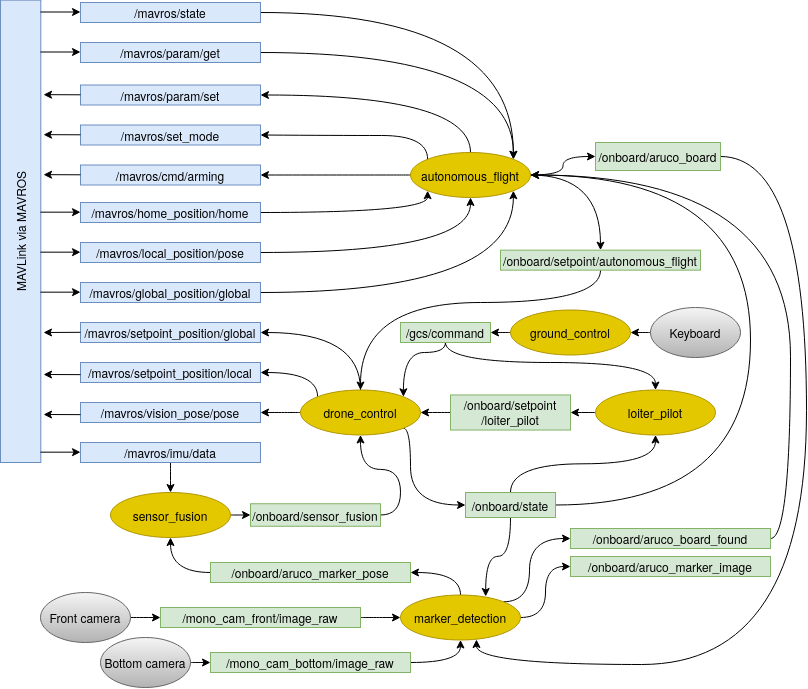
\includegraphics[width=0.95\linewidth]{../Figures/node_communication.png}
    \caption{Overview of the offboard control system. Nodes are labeled yellow, onboard topics green, MAVROS topics blue and hardware gray}
    \label{fig:offboard_control}
\end{figure}

The use of ROS gives the opportunity to subscribe to services from the PX4. These services includes arming the UAV, change parameters like vertical or horizontal speed and much more. This is beneficial because the parameters can be changed during flight in offboard control. This is done using a script called \href{https://github.com/Kenil16/master\_project/blob/master/software/ros\_workspace/src/offboard\_control/uav\_flight\_modes.py}{uav\_flight\_modes.py}. 	

Furthermore, this node publishes the wanted ArUco marker board from which a pose estimation is wanted to be estimated. This is done to distinguish between the GPS to vision marker, world marker on the ground and landing markers. Also the detection of the specified ArUco marker board will be returned as a Boolean to the autonomous flight node by a subscription to the ArUco board found topic. This is done so that the mission will not start until the wanted marker has been located.  

The \textit{\textbf{marker\_detection}} node will analyze the incoming images from the front and bottom camera and estimate the ArUco pose if any markers is located in the image. The theory behind the pose estimation of the ArUco markers will be giving in Section \ref{sec:pose_estimation_using_aruco_markers}. When the pose has been estimated, the result is published to other nodes in the system.

The node which uses this ArUco marker pose is called \textit{\textbf{sensor\_fusion}}. This nodes takes the pose and optimizes it based on fusion with the accelerometer and gyro. This is done to insure that the drone still gets a updated pose estimation even though no markers should be detected in the image. This is very important because the drone uses the ArUco markers as its local coordinate system. The implementation of sensor fusion will be discussed in \ref{sec:sensor_fusion_for_pose_optimization}.  


\todo{Talk about the flight modes script from the services and parameters can be changed }


As seen in Figure \ref{fig:offboard_control}, the drone control node publishes set points to either global position (geographic coordinates), local position (Cartesian coordinates) or vision pose (Cartesian coordinates). The later is a very important aspect of this implementation, which must be mentioned. When the drone gets the pose from a GPS as either   geographic or Cartesian transformed (UTM) coordinates as global or local respectively, the drone uses this coordinate system for navigation. The PX4 auto pilot is relying on an extended Kalman filter for sensor fusion which can be altered from the parameter \textit{EKF2\_AID\_MASK} from the list of services. This uses GPS positions as default, but can be changed to fuse the estimated vision pose instead. By using this configuration, the estimation of the local coordinate system can be changed during flight when the drone is to navigate according to ArUco markers. This way, the use of the build in control schemes for actuator control can still be used, but now the drone navigates according to vision instead of GPS. Hence, a smooth transition from using GPS to vision and vision to GPS can be applied whenever needed. This is also one of the reasons why the pose estimation from the ArUco markers has to be very precise without much variance in its estimates. Otherwise, this could lead to an unstable system where the drone could have trouble positioning itself according to the predefined pose. 

\paragraph{GPS to vision transition}
\label{sec:gps_to_vision_transition}

Because going from one coordinate system to another comes with a cost of an unstable system for a short amount of time, the parameters \textit{MPC\_XY\_VEL\_MAX}, \textit{MPC\_Z\_VEL\_MAX\_DN} and  \textit{MPC\_Z\_VEL\_MAX\_UP} for horizontal and vertical velocities  and \textit{MC\_ROLLRATE\_MAX}, \textit{MC\_PITCHRATE\_MAX} and \textit{MC\_YAWRATE\_MAX} for angular velocities can be set to a very low value before changing between coordinate systems e.g GPS to vision. This insures the drone responds very slowly in the phase of instability caused by the local position and set point position are not aligned i.e. either one is publishing values from the old configuration due to a time delay. Then when the system has settled, the speeds are set back to its initial configuration yielding a smooth transition. This is simply done by inserting a time delay of a few hundreds of milliseconds after a change in the coordinate system to avoid this instability causing problems to the performance of the drone.

However, this  solution does no take into account the contribution of wind, which could make the drone fly away because of decreased rates in angular as well as positional velocities. Moreover, because the ArUco marker board has its own cooridnate system, the local coordinate system of the UAV could potentially be very different in regard to position which would yield errors in the build in Extended Kalman filter of the PX4 if big changes were made in position from one time instant to other.    

A mitigation to this problem is to map the local pose of the drone when it is about to change from using GPS to vision based navigation to that of the vision pose from the ArUco pose estimation. This is done by finding the rotation between the current pose of the drone and that of the ArUco marker board. This is done in Equation \ref{eq:r_uav2aruco}.

\begin{equation}
	r_{uav2aruco} = r_{aruco}^T \cdot r_{uav}
	\label{eq:r_uav2aruco}
\end{equation}

\begin{equation}
	offset = \begin{bmatrix}
						  x_{uav} & x_{aruco}\\
						  y_{uav} & y_{aruco}\\
						  z_{uav} & z_{aruco}\\
						  yaw_{uav} & yaw_{aruco}
					     \end{bmatrix}
\label{eq:offset}
\end{equation}

This rotation defines the difference in the orientation between the ArUco board located on the ground and the UAV before initializing the GPS to vision transition. Furthermore, the position and yaw angle of the UAV is mapped to that of the ArUco marker board which can be seen in Equation \ref{eq:offset}. Because the roll and pitch angles are found negligible in size they are not used in the mapping process. 

Now new updates from the pose can be used to transform the estimation from the ArUco marker board to that of the UAV offset which is seen in Equation \ref{eq:t_aruco_offset}.     

\begin{equation}
	t_{aruco} = \begin{bmatrix}
			   -(x_{offset_{aruco}} - x_{aruco})\\
			   -(y_{offset_{aruco}} - y_{aruco})\\
			   -(z_{offset_{aruco}} - z_{aruco})
			   \end{bmatrix}
\label{eq:t_aruco_offset}
\end{equation}

\begin{equation}
	t_{aruco} = r_{uav2aruco} \cdot t_{aruco}
	\label{eq:t_aruco_transform}
\end{equation}

This vector of the difference between the estimated ArUco position and the offset can be transformed to align to the initial coordinate system of the UAV before the gps to vision transition. This is done in Equation \ref{eq:t_aruco_transform}. 

\begin{equation}
	x = x_{offset_{uav}} + t_{aruco_{x}}
	\label{eq:x_transformed}
\end{equation}

\begin{equation}
	y = y_{offset_{uav}} + t_{aruco_{y}}
	\label{eq:y_transformed}
\end{equation}

\begin{equation}
	z = z_{offset_{uav}} + t_{aruco_{z}}
	\label{eq:z_transformed}
\end{equation}

\begin{equation}
	yaw = yaw_{offset_{uav}} + t_{aruco_{yaw}}
	\label{eq:yaw_transformed}
\end{equation}

When the position has been transformed to align to the original UAV coordinate system they are simply added to the offset of the UAV using Equation \ref{eq:x_transformed},  \ref{eq:y_transformed} and  \ref{eq:z_transformed}. Because both the UAV and ArUco marker board uses coordinate systems with the z-axis pointing up, the yaw angle is just added to the offset as seen in Equation \ref{eq:yaw_transformed} without any transformation needed. These steps are performed in a method called \href{https://github.com/Kenil16/master_project/blob/master/software/ros_workspace/src/offboard_control/transformations_calculations.py} {transformations calculations} which can be seen in GitHub. Hence, the latter solution will be used in the transition from using GPS to vision based navigation to insure a stable and reliable transition. 

This transition of using GPS to vision involves a number of steps. After reaching the target GPS location, the ArUco marker board must be localized, then the drone has to navigate to the board still using GPS coordinates and finally the GPS to vision transition can be initialized if the drone is close enough to the board and estimated poses are stable. A flowchart of this can be seen in Figure \ref{fig:state_machine_gps2vision_transition}. 

\begin{figure}[H]
    \centering
    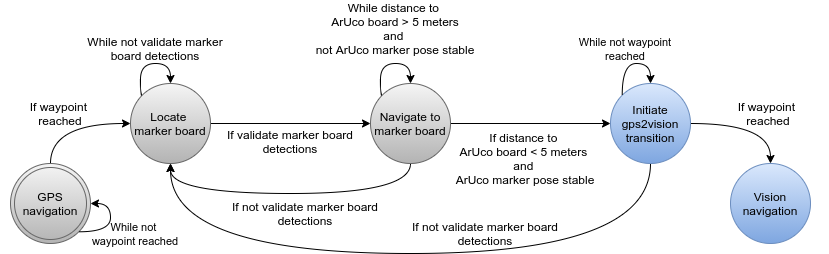
\includegraphics[height=5.0cm]{../Figures/state_machine_gps2vision_transition.png}
    \caption{Illustration of the sub-states when initializing GPS to vision based navigation. Gray boxes defines the use of GPS for pose estimation and blue boxes vision based estimation}
    \label{fig:state_machine_gps2vision_transition}
\end{figure}

As it may be seen, the UAV starts by flying towards a giving predefined waypoint. The approach for \href{https://github.com/Kenil16/master_project/blob/master/software/ros_workspace/src/offboard_control/waypoint_checking.py}{checking if the waypoint has been reached}, is to use the current pose of the UAV and subtracting the target setpoint. Here only the x, y, z and yaw values are used. Then the euclidean distance of the four values are computed and if this value is below a giving threshold (default value is 0.25), the waypoint is reached and the UAV begins to locate the marker board. 

Because there is a risk that the UAV will not see the ArUco marker board located on the wall at its final position, the UAV are set to locate the board by moving in a grid structure of predefined waypoints until the board is found. These waypoints are set from the offset of the final position where the UAV will move in steps of one meter and rotate left to right in steps of 45$^{\circ}$. The UAV will complete this list of waypoints and repeat the process if the board has not been found. If the board is still not found after a predefined number of repetitions, the UAV will land and go into \textit{idle} state and wait for further commands. If the board 
is found, the UAV will begin to navigate to the ArUCo marker board. Because only a single detection of the board could be too unreliable, a sequence of positive detections of the board must be found. This is accomplished by only checking that the board is visible once a second and pushing the result as a Boolean (true/false) on a list with a size of five, where the validate marker board will be true if 80\% of the values on the list have positive observations of the board. This variable is called validate marker board detections in Figure \ref{fig:state_machine_gps2vision_transition}.

Now the UAV will navigate towards the board while keeping its orientation to the board by using Equation \ref{eq:error_navigate_to_board}. 

\begin{equation}
	error = \frac{\frac{imageWidth}{2} - boardCenter_x}{\frac{imageWidth}{2}}
\label{eq:error_navigate_to_board}
\end{equation}    

\begin{equation}
	yaw = error \cdot 30
\label{eq:yaw_navigate_to_board}
\end{equation} 

Here the goal is to have the board be centered in the middle of the image so that the UAV keeps its orientation towards the marker. This results in a normalized error which will be used in a simple P-controller seen in Equation \ref{eq:yaw_navigate_to_board}. Here the maximum change in yaw angle is set to 30$^{\circ}$ which will be based on the normalized error going from zero to one. This limit is chosen to mitigate the possibility of oscillations in the orientation. Now this yaw angle is added to the setpoint yaw, which will keep the UAV orientated towards the board. From results in Section \ref{sec:GPS2Vision_pose_estimation} and \ref{sec:rolling_average_aruco_pose_estimation}, the minimum allowed distance away from the board when initiating GPS to vision transition is found to be approximately five meters with the giving camera resolution and size of the board discussed in Section \ref{sec:pose_estimation_using_aruco_markers}. This is done to make sure that the pose estimates from ArUco markers are reliable. Hence, both the distance to the board and rolling average of latest estimates are used as validation of the estimated pose. The latter is defined by the variable ArUco marker pose stable. If these conditions are met, the drone will initiate GPS to vision transition as seen in Figure \ref{fig:state_machine_gps2vision_transition}.  What goes for both these two substates is that they will fall back to located marker board if they loose sight of the board. 

In the initiate GPS to vision transition, the UAV will use vision pose estimations of the board for navigation using the front camera towards the GPS2Vision marker located on the wall until it is at a predefined location in front of it and then switching to using the bottom camera for the actual vision based navigation which is the last step in the GPS to vision procedure. In the initiate GPS to vision step, the UAV has also been set to keep its orientation towards the marker, but now in a different way. Because the pose estimation is reliable at this point, knowledge of the placement of the GPS2Vision board on the wall can be used along the current pose of the UAV accoding to the pose estimated from vision, to calculate the new yaw angle of the UAV to keep its orientation towards the board. This is done in Equation \ref{eq:delta_x_ori_towards_gps2vision_board}, \ref{eq:delta_y_ori_towards_gps2vision_board} and \ref{eq:yaw_ori_towards_gps2vision_board} where the $aruco_x$ and $aruco_y$ are the current estimate of the ArUco position in x and y. 

\begin{equation}
	\Delta_x = aruco_x - 3.2 - 0.5
	\label{eq:delta_x_ori_towards_gps2vision_board}
\end{equation}

\begin{equation}
	\Delta_y = aruco_y - 3.0
	\label{eq:delta_y_ori_towards_gps2vision_board}
\end{equation}

\begin{equation}
	yaw = atan2(\Delta_y, \Delta_x)
	\label{eq:yaw_ori_towards_gps2vision_board}
\end{equation}

Here 3.2 meters in Equation \ref{eq:delta_x_ori_towards_gps2vision_board} is the distance of the GPS2Vision marker board away from the origin of the board located on the ground and 0.5 meters is to add it to the center of the board. The same goes for Equation \ref{eq:delta_y_ori_towards_gps2vision_board}. The atan2 function is used to calculate this angle in Equation \ref{eq:yaw_ori_towards_gps2vision_board} where 180$^{\circ}$ will be added to this value if the found yaw is below zero. 


\paragraph{Offboard control system}
\label{sec:offboard_control_system}

In order for easy testing of the autonomous system, a set of predefined missions have been set up, which can be executed during a simulation as well as real life testing. For real life execution of these commands, the UAV must be within range of the wireless network or hot-spot created for communication between laptop and the Raspberry Pi on the UAV. However, these commands could also be triggered by using the transmitter for long range communication where the Raspberry Pi using ROS was set to listening for activations of certain switches (high/low) to start the execution of missions from within the script. However, because the UAV will be close to the pilot in this case, a wireless network communication is sufficient for activating missions and control the drone in offboard mode. These keyboard commands can be seen in Table \ref{tab:ros_commands}.  

\begin{table}[H]
\centering
\begin{tabular}{ccc}
\hline
\textbf{Keypress} & \textbf{Node} & \textbf{Action}                                    \\ \hline
t                 & drone\_control & Takeoff + offboard + loiter mode         \\
h                 & drone\_control & Move the drone to home and land         \\
l                 & drone\_control & Switch to loiter control 
\\
wasd              & loiter\_pilot & Forward, left, back and right respectively           \\
qe                & loiter\_pilot & Rotate left or right (yaw) respectively             \\
zx                & loiter\_pilot & Decrease/increase altitude respectively
\\
0                 & drone\_control & Move to GPS locations from vision (\textit{mission})
\\
1                 & drone\_control & Return to landing station one ( \textit{mission})
\\
2                 & drone\_control & Return to landing station two ( \textit{mission})
\\
3                 & drone\_control & Return to landing station three ( \textit{mission})
\\
4                 & drone\_control & GPS2Vision aruco pose estimation test (\textit{mission})  
\\
5                 & drone\_control & Hold ArUco pose test (\textit{mission})  
\\
6                 & drone\_control & GPS2Vision test (\textit{mission})  
\\
7                 & drone\_control & Vision navigation test (\textit{mission})
\\
8                 & drone\_control & Landing test (\textit{mission})  
\end{tabular}
\caption{Table of all possible commands from the GCS}
\label{tab:ros_commands}
\end{table}

Here the UAV can be set to takeoff which will set it into offboard mode and then loiter mode. Because the UAV must get setpoints for the new pose before switching to offboard mode, these are giving before this transition as well as afterwards. The UAV will be in the \textit{takeoff} state until the waypoint giving is reached. Then it will switch to \textit{loiter} state where the UAV can be controlled using keyboard commands as seen in Table \ref{tab:ros_commands} from the node loiter\_pilot. A simplified state machine of these transitions between onboard states of the UAV can be seen in Figure \ref{fig:state_machine_state}. The UAV can be set to return to its home position when it is in \textit{loiter} state. The home position is defined as the place from where the UAV was initiated. This is done in the \textit{Home} state which will result in the UAV switches to \textit{Idle} state when the final home position waypoint has been reached. From \textit{Loiter} state, a number of missions can be executed. 

A number of tests will be performed to evaluate the autonomous system in the simulations. Here the pose estimation of the GPS2Vision board located on the wall must be evaluated to see how reliable the pose estimation is when mowing further away from the board from the \textit{GPS2Vision ArUco pose estimation test}. This is a critical test because this gives an indication of the maximum allowed distance away from this board a safe GPS to vision transition can be performed. This is performed in Section \ref{sec:GPS2Vision_pose_estimation} from where results of this have been used in Section \ref{sec:gps_to_vision_transition} as already discussed. 

The \textit{Hold ArUco pose estimation test} is performed to see how well the UAV is capable of keeping its pose in front of the ArUCo marker boards. The results can be seen in Section \ref{sec:hold_pose_using_aruco_pose_estimation}. This gives an indication of the performance of the control schemes for pose control used within the PX4 autopilot. Moreover, this pose will also be compared to that of the ground truth for performance evaluation. Results from this test will be used in the creation of sensor fusion discussed in Section \ref{sec:sensor_fusion}.

The \textit{GPS to vision test} was performed to evaluate the performance of the GPS to vision transition discussed in Section \ref{sec:gps_to_vision_transition}. This test includes all steps from using GPS, to locate the marker board, navigate to the marker board and initialize the GPS to vision transition. Results of this can be seen in Section \ref{sec:gps2vision_transition}.

In the \textit{Vision based navigation test}, the performance of using the bottom camera to navigate the drone is evaluated. In this test sensor fusion is used in the indoor environment with a number of different configuration of markers located on the ground. Results can be seen in Section \ref{sec:vision_based_navigation}. 

Finally, the vision based landing procedure is tested in \textit{Landing test}. Here the UAV will move between landing stations and land in front of the landing boards where the final landing position will be compared to that of the ground truth to evaluate the performance from the wanted setpoint location. Results can be seen in Section \ref{sec:vision_based_landing}

From being in the \textit{Loiter} state, the UAV can be set to return to one of the landing stations. That way the UAV can be set to execute a route and then afterwards return to the landing stations specified by one, two and three. When the UAV has landed, it will be in \textit{Vision landed} state, where the pose is still calculated using vision from the ArUco marker landing boards. When wanted, the UAV can again execute a route by making it return to using GPS coordinates after moving outside the vision navigation area. This can be seen in Figure \ref{fig:state_machine_state}. 

\begin{figure}[H]
    \centering
    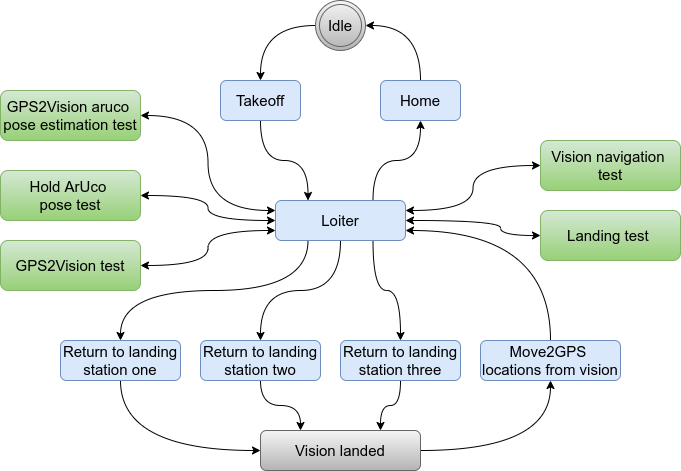
\includegraphics[height=8.0cm]{../Figures/state_machine_state.png}
    \caption{A simplified state machine of the onboard states of the UAV. Green boxes defines the states with the intention of testing the autonomous flight system. Blue boxes defines the actual autonomous system from where the UAV can be controlled from either keyboard commands in \textit{Loiter} or return to a landing station from using GPS or being at a landing station and then move to a GPS location from using vision to GPS coordinates}
    \label{fig:state_machine_state}
\end{figure}

A bash script has been created for automatic execution of tests which can be seen in Listing \ref{lst:bash_script_for_automatic_execution_of_test}. This is done to make the execution of tests scalable and easy to perform. As seen in Listing \ref{lst:bash_script_for_automatic_execution_of_test}, a directory is created if not already defined. Data from each test is saved in the data directory which is copied to the test directory for each execution. This is done so that all data from all simulations can be analyzed afterwards. A predefined number of tests can be set which will be executed in each run defined by iterations. They way the program terminates in each run, is to call \textit{rospy.signal\_shutdown("Test completed!")} from within the end of the code e.g \href{https://github.com/Kenil16/master\_project/blob/0ca6b6205ecfd8cc6a819d7cd30c979fcd39e6e8/software/ros\_workspace/src/offboard\_control/autonomous\_flight.py#L266}{GPS2Vision\_test} from the \href{https://github.com/Kenil16/master\_project/blob/master/software/ros\_workspace/src/offboard\_control/autonomous\_flight.py}{autonomous\_flight.py} script in offboard control. However, to be able so make a single node terminate the entire program \textit{required="true"} must be added in the initialization of the giving node from where the shutdown takes places. This can be seen in the created launch file \href{https://github.com/Kenil16/master\_project/blob/0ca6b6205ecfd8cc6a819d7cd30c979fcd39e6e8/software/ros\_workspace/PX4-software/launch/gazebo\_sim\_v1.0.launch#L63}{gazebo\_sim\_v1.0.launch}. This roslaunch file is used throughout the simulations which can be executed directly from the terminal. The way to start a simulation can be seen in line 12 in Listing \ref{lst:bash_script_for_automatic_execution_of_test}. Here the wanted world can be giving as input to the program, along with the wanted onboard state of the UAV. By giving this state as input to the program, tests can be started directly without having to initiate them by using keyboard commands. This gives the possibility of starting roslaunch in headless mode, which means that no GUI is used. The program will simply be executed silently as a background process which also requires less resources to run. Furthermore, the starting pose of the UAV is giving as input as well. This pose will have to be changed accordingly to the appropriate test from where the test is to be executed. 


\definecolor{lightgreen}{rgb}{0.56, 0.93, 0.56}
\definecolor{moonstoneblue}{rgb}{0.45, 0.66, 0.76}
\begin{listing}[H] 
\begin{tcolorbox}[
    enhanced,
    attach boxed title to top left={xshift=6mm,yshift=-3mm},
    colback=lightgreen!20,
    colframe=lightgreen,
    fonttitle=\bfseries\color{black},
]
\begin{minted}[ numbersep=6pt, linenos=true, breaklines=true, breakanywhere=true, mathescape, escapeinside=||,fontsize=\small]{bash}
#!/bin/bash
#Specify data analysis directory, name of data file, name for the test and number of runs
DIRECTORY="../../data/analyse_vision_navigation_pose_estimation/test5_one_pattern_missing_markers_wear_board/"
data_file="../../data/sensor_fusion_data.txt"
test_name="test"
iterations=20
#Run for nunmber of test times 
if [ ! -d "$DIRECTORY" ]; then echo "Dir does not exist" 
mkdir -p $DIRECTORY else echo "Dir does exist"
fi
for (( c=1; c<=$iterations; c++ ))
do roslaunch px4 gazebo_sim_v1.0.launch worlds:=optitrack_big_board_onepattern_missing_markers_wear.world drone_control_args:="vision_navigation_test" x:=-3.0 y:=0.0 headless:=true gui:=false 
cat $data_file > "$DIRECTORY$test_name$c.txt" 
echo "Test $c completed!"
done

\end{minted}
\end{tcolorbox}
\caption{Bash script for automatic execution of test}
\label{lst:bash_script_for_automatic_execution_of_test}    
\end{listing}   

\paragraph{Software setup} 

Additional software will have to be installed and configured in order to use ROS. For performing conversions between UTM, geographic, local Cartesian coordinates etc.  \href{https://geographiclib.sourceforge.io/}{GeographicLib} is used. This is mandatory in order to use MAVROS along with PX4. This can be installed using Listing \ref{lst:install_geographiclib_datasets}.

\definecolor{lightgreen}{rgb}{0.56, 0.93, 0.56}
\definecolor{moonstoneblue}{rgb}{0.45, 0.66, 0.76}
\begin{listing}[H] 
\begin{tcolorbox}[
    enhanced,
    attach boxed title to top left={xshift=6mm,yshift=-3mm},
    colback=lightgreen!20,
    colframe=lightgreen,
    fonttitle=\bfseries\color{black},
]
\begin{minted}[ numbersep=6pt, linenos=true, breaklines=true, breakanywhere=true, mathescape, escapeinside=||,fontsize=\small]{bash}
#Update system before installation 
$ Sudo update
#Fetch the sofware, change permissions and execute script from terminal
$ wget https://raw.githubusercontent.com/mavlink/mavros/master/mavros/scripts/install_geographiclib_datasets.sh
$ sudo chmod 755 install_geographiclib_datasets.sh
$ sudo ./install_geographiclib_datasets.sh
\end{minted}
\end{tcolorbox}
\caption{Installation of the Geographiclib datasets as dependencies for MAVROS}
\label{lst:install_geographiclib_datasets}    
\end{listing}

Because the simulations will be running on an Ubuntu 18.04.5 LTS (Bionic Beaver) 64-bit desktop operating system and server edition for the Raspberry Pi, ROS melodic will be used. Furthermore, the Raspberry Pi does not need the full installation of ROS due to the fact that no GUI is used as the communication between the Raspberry Pi and Laptop will be through SSH from the terminal. Therefore, ROS base will be installed on the Raspberry Pi and the full desktop version installed on the laptop. 

The system must be configured to accept packages from \href{http://wiki.ros.org/melodic/Installation/Ubuntu}{ROS} along with setting up the cryptographic keys for package authentication. When this is done, ROS can be installed which is seen in Listing \ref{lst:ros_installation}. Here the full edition of MAVROS will be installed for communication as already discussed. 

\begin{listing}[H] 
\begin{tcolorbox}[
    enhanced,
    attach boxed title to top left={xshift=6mm,yshift=-3mm},
    colback=lightgreen!20,
    colframe=lightgreen,
    fonttitle=\bfseries\color{black},
]
\begin{minted}[ numbersep=6pt, linenos=true, breaklines=true, breakanywhere=true, mathescape, escapeinside=||,fontsize=\small]{bash}
#Setup your sources.list
$ sudo sh -c 'echo "deb http://packages.ros.org/ros/ubuntu $(lsb_release -sc) main" > /etc/apt/sources.list.d/ros-latest.list'
#Set up your keys
$ sudo apt-key adv --keyserver 'hkp://keyserver.ubuntu.com:80' --recv-key C1CF6E31E6BADE8868B172B4F42ED6FBAB17C654
#Install ROS dependencies 
$ sudo apt install python-rosdep python-rosinstall python-rosinstall-generator python-wstool build-essential python-rosdep
#Installation
$ sudo apt install ros-melodic-desktop-full
#Install mavros along with extra packages
$ sudo apt install ros-melodic-mavros ros-melodic-mavros-extras -y python-catkin-tools -y ros-melodic-hector-gazebo-plugins dvipng
\end{minted}
\end{tcolorbox}
\caption{Installation of ROS with required dependencies}
\label{lst:ros_installation}    
\end{listing}   

For easy debugging of the system, rqt is installed. This is a software framework which includes plugins for varies GUIs e.g plotting, graphs and image viewing. This will utilize the possibility of visualizing the images from the front and bottom cameras of the UAV, to see the detected ArUco boards. Moreover, to enable ROS to access images from attached cameras from the USB, the USB camera plugin will be installed on the Raspberry Pi using line 4 in Listing \ref{lst:software_related_installations_for_ros}.  

\begin{listing}[H] 
\begin{tcolorbox}[
    enhanced,
    attach boxed title to top left={xshift=6mm,yshift=-3mm},
    colback=lightgreen!20,
    colframe=lightgreen,
    fonttitle=\bfseries\color{black},
]
\begin{minted}[ numbersep=6pt, linenos=true, breaklines=true, breakanywhere=true, mathescape, escapeinside=||,fontsize=\small]{bash}
#Install packages for visualization of video stream (ros rqt)
$ sudo apt-get install ros-melodic-rqt ros-melodic-rqt-common-plugins
#Install packages for USB readings using ROS
$ sudo apt-get install ros-melodic-usb-cam ros-melodic-image-transport ros-melodic-image-transport-plugins ros-melodic-image-transport-plugins ros-melodic-camera-info-manager
#Install packages fto be able to execute scrips
$ sudo apt-get install liblapack-dev gfortran libblas-dev libxml2-dev libxslt-dev python-dev python-pip
$ pip install pathlib pymavlink pandas scipy opencv-contrib-python matplotlib numpy
\end{minted}
\end{tcolorbox}
\caption{Dependencies for created ROS nodes and visualization}
\label{lst:software_related_installations_for_ros}    
\end{listing}   

For easy creation of paths for files \textit{pathlib} is used. For communication along MAVROS a python version of \textit{pymavlink} is installed. \textit{Pandas} and \textit{matplotlib} will be used for data analysis for plotting, \textit{scipy} in the creation of the Unscented Kalman filter and \textit{opencv-contrib-python} for enabling the use of OpenCV for computer vision algorithms e.g detecting ArUco marker boards where the \textit{contrib} edition of OpenCV includes the  mandatory ArUco libraries. Lastly \textit{numpy} is used for data structuring.      

\subsubsection{PX4 autopilot}
\label{sec:px4_flight_stack}

PX4 is an open source control software for unmanned vehicles. PX4 uses software in the loop (SITL) for simulations of a given unit before real world testing. The flight stack runs on a computer which could be any unit on the same network. For operation on real hardware,    

\begin{figure}[H]
    \centering
    \begin{subfigure}[b]{0.48
    \linewidth}
        \centering
        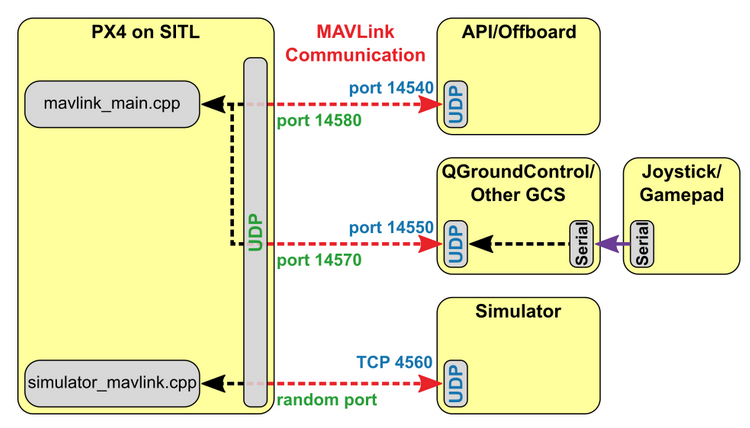
\includegraphics[width=1\linewidth]{../Figures/px4_sitl.png}
        \caption{}
        \label{fig:mavlink_comminication}
    \end{subfigure}
      \hskip 10ex
    \begin{subfigure}[b]{0.26\linewidth}
        \centering
        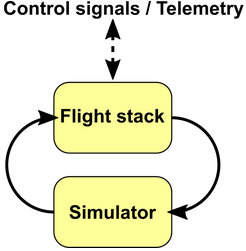
\includegraphics[width=1\linewidth]{../Figures/simulator_mavlink_api.png}
        \caption{}
        \label{fig:simulator_mavlink_api}
    \end{subfigure}
    \caption{Illustrations of the message handling in the SITL simulation environment \cite{px4Autopilot}}
    \label{fig:sitl_simulation_enviroment}
\end{figure}

In Figure \ref{fig:simulator_mavlink_api}, a high level view of the communication between the PX4 flight stack and simulation environment (Gazebo) can be seen. Sensor readings like GPS, IMU data etc. are passed to the PX4 flight controller which returns control outputs (motor actuator commands) to the simulation according to sensor readings. 

The transmission of messages between PX4 and external programs happens using  the user datagram protocol (UDP) ports for MAVLink communication. This is illustrated in Figure \ref{fig:mavlink_comminication}. Here a number of ports are associated to different applications. The UDP Port 14540 is used for offboard control communication which will be python scripts running in the simulation or on the Raspberry Pi for autonomous flight using information from sensors e.g. vision feedback. The UDP port 14550 is used for communicating with ground control stations (GCS). QGroundControl, which is explained in Section \ref{sec:qgroundcontrol},  will be used which offers many features like sensor calibration, radio setup and calibration of transmitters, predefined air frame selection for different drones etc. Moreover, parameters for position and attitude control, velocity limits and the like can be changed during flights. However, these parameters can also be changed using ROS in the offboard control script, which will be explained in Section \ref{sec:ros}. The last port, UDP 4560, will be used for transmission of messages between PX4 and the simulation environment.

\paragraph{Software setup}

This implementation of PX4 SITL requires firmware vision 1.11.0 to work correctly. This setup relies on the PX4 firmware being installed in the \textit{home} directory of the user, but can be modified to another installation directory with minor configurations. A walk-trough of these initial steps for installing and setting up of the firmware can be seen in Listing \ref{lst:installation_px4_sitl}. 

\begin{listing}[H] 
\begin{tcolorbox}[
    enhanced,
    attach boxed title to top left={xshift=6mm,yshift=-3mm},
    colback=lightgreen!20,
    colframe=lightgreen,
    fonttitle=\bfseries\color{black},
]
\begin{minted}[ numbersep=6pt, linenos=true, breaklines=true, breakanywhere=true, mathescape, escapeinside=||,fontsize=\small]{bash}
#Update system 
$ Sudo update 
#Initialize PX4 SITL environment from your home folder
$ cd ~
$ mkdir PX4_SITL
$ cd PX4_SITL
$ git clone https://github.com/PX4/Firmware.git --branch v1.11.0
$ cd Firmware
$ git submodule update --init --recursive
#Make symlink to user software models to PX4 SITL
$ cd software/ros_workspace/
$ ln -s $PWD/PX4-software/init.d-posix/* /home/$USER/PX4_SITL/Firmware/ROMFS/px4fmu_common/init.d-posix/
$ ln -s $PWD/PX4-software/mixers/* /home/$USER/PX4_SITL/Firmware/ROMFS/px4fmu_common/mixers/
$ ln -s $PWD/PX4-software/models/* /home/$USER/PX4_SITL/Firmware/Tools/sitl_gazebo/models/
$ ln -s $PWD/PX4-software/worlds/* /home/$USER/PX4_SITL/Firmware/Tools/sitl_gazebo/worlds/
$ ln -s $PWD/PX4-software/launch/* /home/$USER/PX4_SITL/Firmware/launch/
#Build the PX4 SITL firmware
$ cd /home/$USER/PX4_SITL/Firmware
$ DONT_RUN=1 make px4_sitl_default gazebo
\end{minted}
\end{tcolorbox}
\caption{Installation and setting up of the PX4 SITL firmware}
\label{lst:installation_px4_sitl}    
\end{listing}  

Here the PX4 firmware is fetched and installed in a directory called \textit{PX4\_SITL} from where dynamic links have been created from a ROS workspace. This configuration was made to easily link updates made in files from \textit{init.d-posix}, \textit{mixers}, \textit{models}, \textit{worlds} and \textit{launch} directories. The \textit{init.d-posix} directory is used for parameter initialization for the vehicle at startup which contains files for the used \textit{sdu model drone} to be used in simulations. The \textit{mixers} directory contains files for the motor configuration of the vehicle. In this case it would be configurations for an hexarotor drone. The directory for \textit{models} contains files to be used in simulations like the \textit{sdu drone model} seen in Figure  \ref{fig:sdu_drone} and models created in Section \ref{sec:3d_modeling_for_gazebo_simulations}. The \textit{worlds} directory includes all world files to be used in the simulation which were defined in Section \ref{sec:3d_modeling_for_gazebo_simulations}. Lastly, the \textit{launch} directory stores the launch files to be used for running the PX4 SITL simulation wrapped in ROS.   

Whenever a new terminal is opened, the variables of the software has to be exported with the ROS workspace and firmware sourced so that the PX4 simulation can be started. In order to do this is one step, a script has been created as seen in Listing \ref{lst:setup_gazebo.bash}. 

\begin{listing}[H] 
\begin{tcolorbox}[
    enhanced,
    attach boxed title to top left={xshift=6mm,yshift=-3mm},
    colback=lightgreen!20,
    colframe=lightgreen,
    fonttitle=\bfseries\color{black},
]
\begin{minted}[ numbersep=6pt, linenos=true, breaklines=true, breakanywhere=true, mathescape, escapeinside=||,fontsize=\small]{bash}
#!/bin/bash
$ source devel/setup.bash
$ source ~/PX4_SITL/Firmware/Tools/setup_gazebo.bash ~/PX4_SITL/Firmware ~/PX4_SITL/Firmware/build/px4_sitl_default
$ export ROS_PACKAGE_PATH=$ROS_PACKAGE_PATH:~/PX4_SITL/Firmware
$ export ROS_PACKAGE_PATH=$ROS_PACKAGE_PATH:~/PX4_SITL/Firmware/Tools/sitl_gazebo
$ export GAZEBO_PLUGIN_PATH=${GAZEBO_PLUGIN_PATH}:~/catkin_ws/devel/lib/
\end{minted}
\end{tcolorbox}
\caption{Setup gazebo and PX4 from ROS workspace}
\label{lst:setup_gazebo.bash}    
\end{listing}  

This script can either be run from the ROS workspace or past to the \textit{.bashrc} file to be executed every time a new terminal is opened for easy initialization. 


\subsection{Pose estimation using ArUco markers}
\label{sec:pose_estimation_using_aruco_markers}

\todo{Somethig needs to be done here. Either a more thorough desciption of the aruco pose estimation or other methods in regard to pose estimation using markers could e mentioned. Maybe look at N-fold-markers. How does this pose estimation work and why could that the an alternative to using aruco markers - bring images and calculations for that pose estimation procedure.}

This section deals which pose estimation of ArUco markers to be used as the local coordinate system for the drone for vision based navigation. 

A number of visual markers could be used for pose estimation e.g ArUco markers, AprilTag or QR-codes just to name a few. However, to achieve real-time performance, the latter cannot be used due to large amount of data in the marker. This is not the case with ArUco markers and AprilTag which also yields good performance in regards to detection accuracy and a low error rate. \cite{visualmarkers} 

Because the ArUco markers have been shown to have high performance along with libraries for ArUco marker boards for better precision, ArUco markers will be used for pose estimation.       Furthermore, these estimations is made using OpenCVs marker detection and pose estimation for ArUco markers.

\subsubsection{ArUco marker detection}

The ArUco marker consists of a black border with an inner binary matrix (bits) which defines its ID. This inner binary matrix is called the binary codification of the marker. To detect a marker, candidates in the image are first analyzed where adaptive thresholding is applied to the image and afterwards extracting contours which have to be square in order to be categorized as a marker candidate. When the candidates have been found, a perspective transformation is applied to each of them, to remove distortion in the images. This can be seen in Figure \ref{fig:aruco_detection1} and \ref{fig:aruco_detection2} where a marker candidate are giving to the algorithm for further processing. In this step Utsu thresholding have been used. Then the image can be divided into cells which corresponds to the predefined size of the marker (bits) and corresponding border size. In each cell, the number of black and white pixels are determined in order to categories the candidate marker to belong to a specific dictionary where it is finally evaluated to be and ArUco marker or not. These steps can be seen in Figure \ref{fig:aruco_detection3}, \ref{fig:aruco_detection4} and \ref{fig:aruco_detection5}.       


\begin{figure}[H]
    \centering
    \begin{subfigure}[b]{.1525\textwidth}
        \centering
        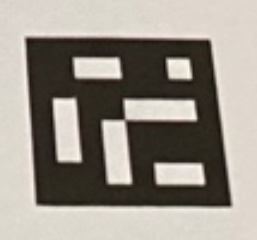
\includegraphics[width=1\linewidth]{../Figures/aruco_detection1.png}
        \caption{}
        \label{fig:aruco_detection1}
        %\vspace*{0.1cm}
    \end{subfigure}
    \begin{subfigure}[b]{.15\textwidth}
        \centering
        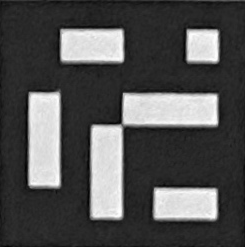
\includegraphics[width=1\linewidth]{../Figures/aruco_detection2.png}
        \caption{}
        \label{fig:aruco_detection2}
    \end{subfigure}
        \begin{subfigure}[b]{.15\textwidth}
        \centering
        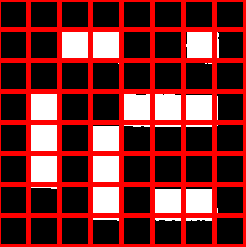
\includegraphics[width=1\linewidth]{../Figures/aruco_detection3.png}
        \caption{}
        \label{fig:aruco_detection3}
    \end{subfigure}
        \begin{subfigure}[b]{.15\textwidth}
        \centering
        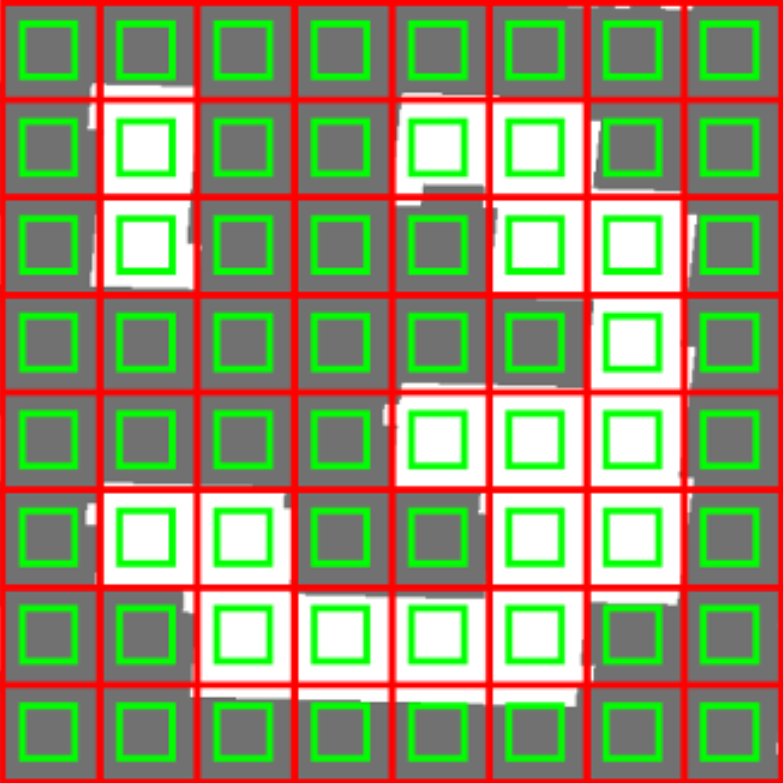
\includegraphics[width=1\linewidth]{../Figures/aruco_detection4.png}
        \caption{}
        \label{fig:aruco_detection4}
    \end{subfigure}
        \begin{subfigure}[b]{.154\textwidth}
        \centering
        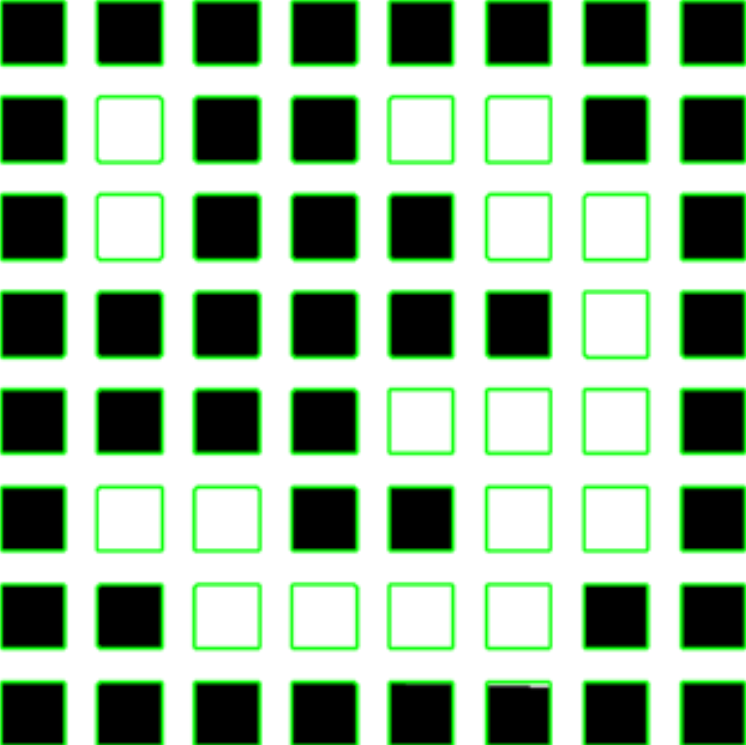
\includegraphics[width=1\linewidth]{../Figures/aruco_detection5.png}
        \caption{}
        \label{fig:aruco_detection5}
         \vspace{-0.05cm}
    \end{subfigure}
    \caption{Illustration of the procedures of ArUco marker detection \cite{arucoMarkerDetection}}
    \label{fig:aruco_detection_procedure}
  
\end{figure}

\subsubsection{ArUco pose estimation}

Knowing the size of the marker, defined when creating the ArUco marker board, the intrinsic and corresponding distortion parameters in the camera and the found corners of each marker, a pose estimation can now be performed. For pose estimation, OpenCV uses an implementation of Levenberg-Marquardt optimization for solving the perspective-n-point (PnP) which estimates the pose of a camera in respect to the ArUco board giving a set of 3D points in the board reference system and there corresponding 2D projections in the image. The model for this can be seen in Equation \ref{eq:pnp} and simplified in Equation \ref{eq:pnp_simplified}.

\begin{equation}
	s	
	\begin{bmatrix}
		u\\
		v\\
		1
	\end{bmatrix}
	=
	\begin{bmatrix}
		f_x & \gamma & u_0\\
		0 & f_y & v_0\\
		0 & 0 & 1
	\end{bmatrix}
	\begin{bmatrix}
		r_11 & r_12 & 13 & t_1\\
		r_21 & r_22 & r23 & t_2 \\
		r_31 & r_32 & r_33 & t_3 \\
	\end{bmatrix}
	\begin{bmatrix}
		X\\
		Y\\
		Z\\
		1
	\end{bmatrix}
	\label{eq:pnp}
\end{equation}

\begin{equation}
	s \cdot p_{c} = K \cdot[R|T] \cdot p_{w}
	\label{eq:pnp_simplified}
\end{equation}

Here $f_x$ and $f_y$ defines focal lengths, $u_0$ and $v_0$ are the principle points which are expected to be the center of the image, $\gamma$ the skew parameter and $s$ a scaling factor for the image. The two vectors $p_c$ and $p_w$ defines the 2D and 3D points for the projection in the image and known locations of the marker corners respectively. Hence, the rotation matrix $R$ and translation vector $T$ can be estimated, which yields a rotation and translation of the board in respect to the camera \cite{pnp} \cite{estimatePoseBoard}. 

As defined in Section \ref{sec:3d_modeling_for_gazebo_simulations}, the drone will use the marker located on the ground as the local coordinate system. Because the GPS to vision marker is located on the wall to the entrance of the building and three landing markers are used when the drone is to land, the $Marker_{GPS2vision}$, $Marker_{landing_1}$, $Marker_{landing_2}$ and $Marker_{landing_3}$ must be transformed to align with the local coordinate system. An illustration of the placement of these marker boards visualized from above can be seen in Figure \ref{fig:2d_view_aruco_coordinate_systems}. It may be noticed that the GPS to vision marker and all landing makers have the same orientation and differs only in translation. In this configuration, the bottom camera of the drone is used for pose estimation of the ground marker and front camera for the GPS to vision and landing markers. This yields two different configurations as seen in Figure \ref{fig:3d_view_aruco_coordinate_systems}. In Figure \ref{fig:3d_view_aruco_front_camera}, the drone is considered to hover in front of the GPS to vision marker. Here four coordinate systems are illustrated namely the marker located on the ground, the drone, the front camera attached on the drone and the GPS to vision marker. To get the pose of the drone in respect to the ground marker, the rotation and translation of the camera w.r.t  the marker board must be found using Equation \ref{eq:translation_from_board2cam}. Here the transpose of the rotation vector named $r_{vec}$ is multiplied with the translation vector $t_{vec}$ to give a translation from the camera to the marker board. This has to be done because the output $r_{vec}$ and $t_{vec}$ from the pose estimation using OpenCV are given from the marker board w.r.t the camera \cite{theExtrinsicCameraMatrix}. 

\begin{equation}
	t = -r_{vec}^T t_{vec} 
	\label{eq:translation_from_board2cam}  
\end{equation} 

This initial step goes for both cameras. Now to get the pose of the drone w.r.t the ground marker, Equation \ref{eq:translation_drone2ground_gps2vision} is used.

\begin{equation}
	P^{Drone}_{Marker_{Ground}} = T^{Marker_{GPS2vision}}_{Marker_{ground}} \cdot T^{Drone}_{Camera_{front}} \cdot t
	\label{eq:translation_drone2ground_gps2vision} 
\end{equation}

\begin{figure}[H]
    \centering
    \begin{subfigure}[t]{.4\textwidth}
        \centering
    \scalebox{0.75}{
\begin{tikzpicture}[scale=5]

    \begin{scope}[
            yshift=-3.5, xshift=16, every node/.append style={
            yslant=-0,xslant=0},yslant=0,xslant=0]
            
    \node[
          opacity=0.5, anchor=south east,inner sep=0pt] at (0,0) 
           {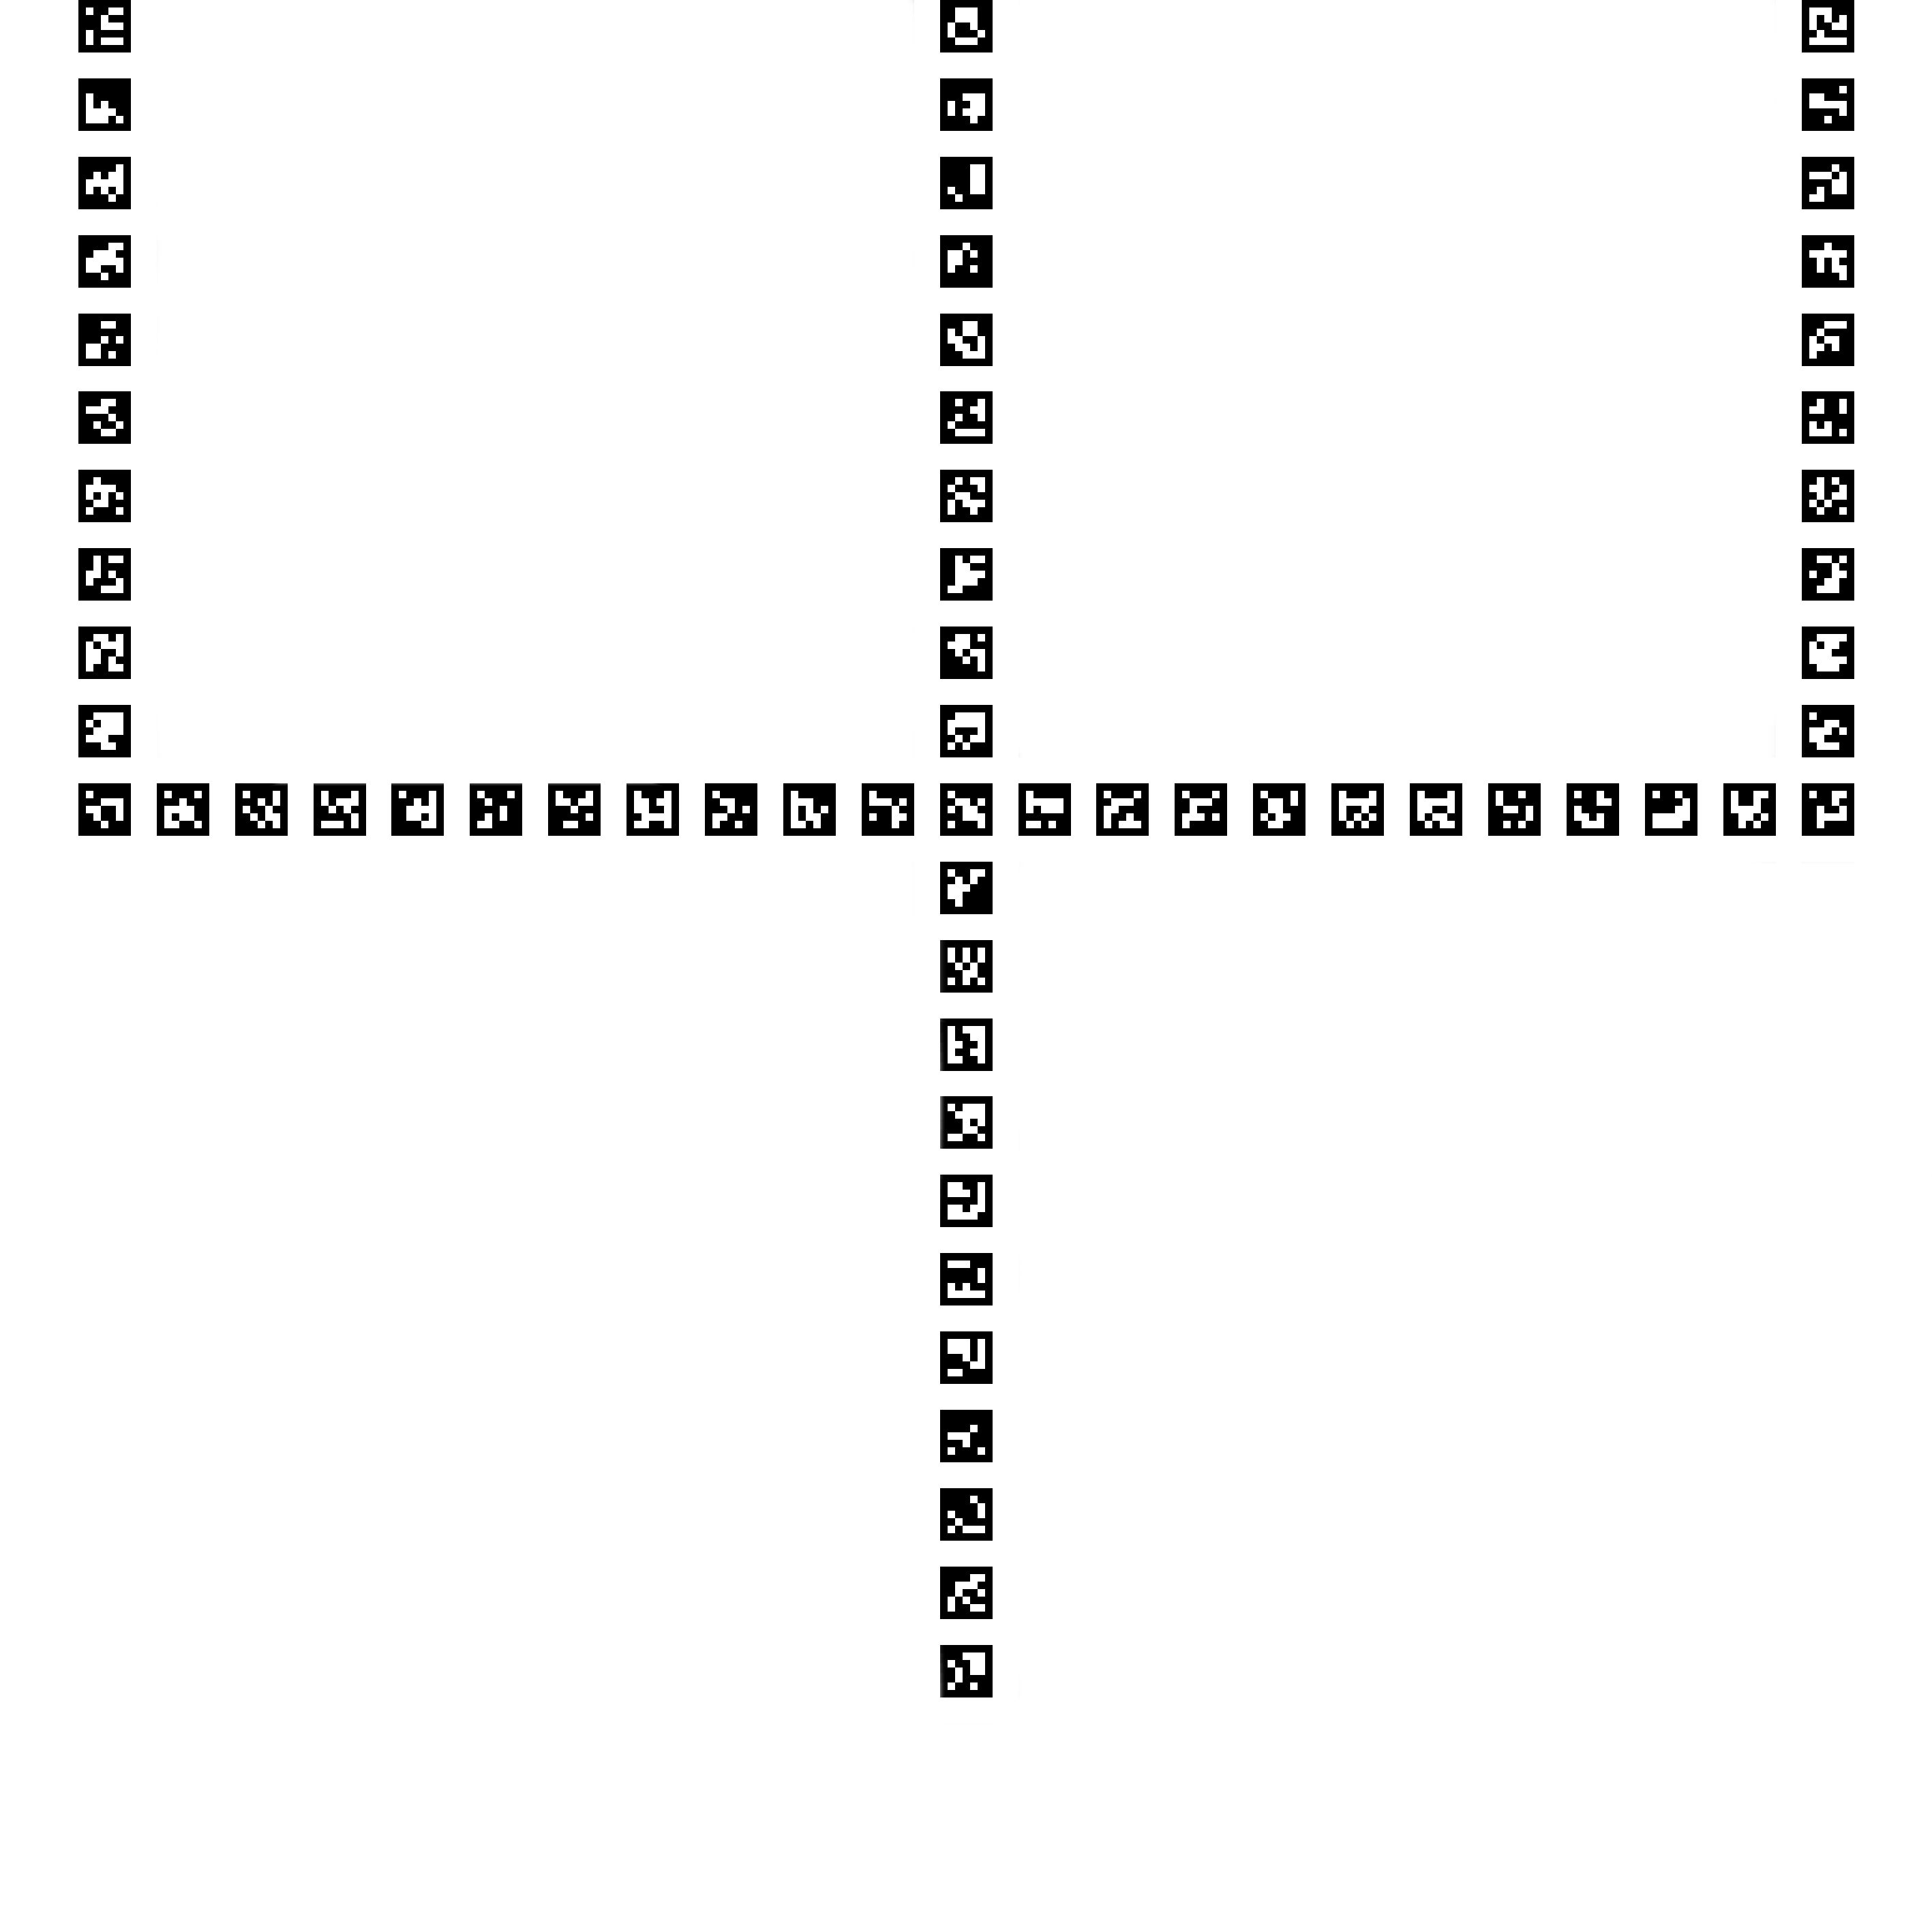
\includegraphics[width=6cm]{../Figures/original_one_pattern_aruco.png}}; 

    \end{scope}

%Draw ground marker (world)
\draw[->, red] (-0.6,0) -- (-0.3,0) node[right]{$x$};
\draw[->, green] (-0.6,0) -- (-0.6,0.3) node[above]{$y$};
\node[align=center] at (-1.0, 0.2) (ori) {$Marker_{ground}$};
\draw[->,help lines,shorten >=3pt] (ori) .. controls (-0.8,0.13) and (-0.75, 0.1) .. (-0.61, 0.02);

%Draw GPS to vision marker
\draw[->, red] (-0.1,0.35) -- (0.2,0.35) node[right]{$x$};
\draw[->, blue] (-0.1,0.35) -- (-0.1,0.05) node[below]{$z$};
\node[align=center] at (0.4, 0.1) (ori) {$Marker_{GPS2vision}$};
\draw[->, black, help lines,shorten >=3pt] (ori) .. controls (0.2,0.15) and (0.1, 0.2) .. (-0.1, 0.35);

%Draw landing marker one
\draw[->, red] (-0.62,1.30) -- (-0.32,1.3) node[right]{$x$};
\draw[->, blue] (-0.62,1.30) -- (-0.62,1.0) node[below]{$z$};
\node[align=center] at (-1.1, 1.0) (ori) {$Marker_{landing_1}$};
\draw[->, black, help lines,shorten >=3pt] (ori) .. controls (-1.0,1.1) and (-0.95, 1.2) .. (-0.62, 1.30);

%Draw Glanding marker two
\draw[->, red] (-0.08,1.3) -- (0.18,1.3) node[right]{$x$};
\draw[->, blue] (-0.08,1.3) -- (-0.08,1.0) node[below]{$z$};
\node[align=center] at (0.4, 1.5) (ori) {$Marker_{landing_2}$};
\draw[->, black, help lines,shorten >=3pt] (ori) .. controls (0.4,1.4) and (0.0, 1.4) .. (-0.076, 1.3);

%Draw Glanding marker two
\draw[->, red] (0.45,1.3) -- (0.75,1.3) node[right]{$x$};
\draw[->, blue] (0.45,1.3) -- (0.45,1.0) node[below]{$z$};
\node[align=center] at (1.0, 1.1) (ori) {$Marker_{landing_3}$};
\draw[->, black, help lines,shorten >=3pt] (ori) .. controls (0.6,1.1) and (0.7, 1.22) .. (0.45, 1.28);

\end{tikzpicture}}
    \caption{}
    \label{fig:2d_view_aruco_coordinate_systems}
    \end{subfigure}
    \hspace{9.5em}
    \begin{subfigure}[t]{.33\textwidth}
        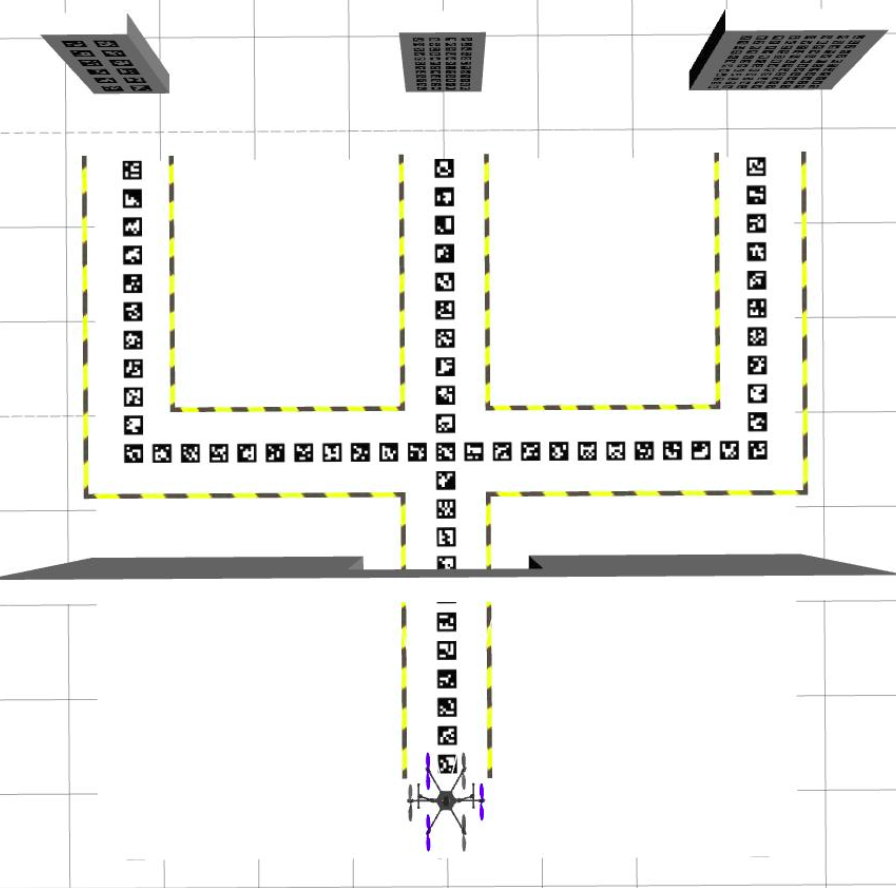
\includegraphics[angle=-0.5,width=1\linewidth]{../Figures/3d-modeling/one_pattern_board_top_view.png}
        \hspace{-0.0em}
        \caption{}
        \label{fig:2d_view_aruco_marker_board}
    \end{subfigure}
    \caption{Visualization of the coordinate systems of the ArUco marker boards in the simulation seen from above. The actual coordinate systems can be seen in Figure \ref{fig:2d_view_aruco_coordinate_systems} and an image of the simulation environment in Figure \ref{fig:2d_view_aruco_marker_board} for easy comparison}
    \label{fig:3d_view_aruco_coordinate_systems}
\end{figure}

\begin{figure}[H]
    \centering
    \begin{subfigure}[t]{.48\textwidth}
        \centering
\scalebox{1.0}{\tdplotsetmaincoords{60}{110}

\newcommand{\tdseteulerxyz}{
\renewcommand{\tdplotcalctransformrotmain}{%
%perform some trig for the Euler transformation
\tdplotsinandcos{\sinalpha}{\cosalpha}{\tdplotalpha} 
\tdplotsinandcos{\sinbeta}{\cosbeta}{\tdplotbeta}
\tdplotsinandcos{\singamma}{\cosgamma}{\tdplotgamma}
%
\tdplotmult{\sasb}{\sinalpha}{\sinbeta}
\tdplotmult{\sasg}{\sinalpha}{\singamma}
\tdplotmult{\sasbsg}{\sasb}{\singamma}
%
\tdplotmult{\sacb}{\sinalpha}{\cosbeta}
\tdplotmult{\sacg}{\sinalpha}{\cosgamma}
\tdplotmult{\sasbcg}{\sasb}{\cosgamma}
%
\tdplotmult{\casb}{\cosalpha}{\sinbeta}
\tdplotmult{\cacb}{\cosalpha}{\cosbeta}
\tdplotmult{\cacg}{\cosalpha}{\cosgamma}
\tdplotmult{\casg}{\cosalpha}{\singamma}
%
\tdplotmult{\cbsg}{\cosbeta}{\singamma}
\tdplotmult{\cbcg}{\cosbeta}{\cosgamma}
%
\tdplotmult{\casbsg}{\casb}{\singamma}
\tdplotmult{\casbcg}{\casb}{\cosgamma}
%
%determine rotation matrix elements for Euler transformation
\pgfmathsetmacro{\raaeul}{\cacb}
\pgfmathsetmacro{\rabeul}{\casbsg - \sacg}
\pgfmathsetmacro{\raceul}{\sasg + \casbcg}
\pgfmathsetmacro{\rbaeul}{\sacb}
\pgfmathsetmacro{\rbbeul}{\sasbsg + \cacg}
\pgfmathsetmacro{\rbceul}{\sasbcg - \casg}
\pgfmathsetmacro{\rcaeul}{-\sinbeta}
\pgfmathsetmacro{\rcbeul}{\cbsg}
\pgfmathsetmacro{\rcceul}{\cbcg}
}
}
\tdseteulerxyz

\begin{tikzpicture}[scale=3,tdplot_main_coords]


%Ground marker 
\tdplotsetrotatedcoords{45}{0}{0}
\draw[thick,red,tdplot_rotated_coords,->] (0,0,0) -- (1.5,0,0) node[anchor=north east]{$x$};
\draw[thick,green,tdplot_rotated_coords,->] (0,0,0) -- (0,1.5,0) node[anchor=north west]{$y$};
\draw[thick,blue,tdplot_rotated_coords,->] (0,0,0) -- (0,0,1.5) node[anchor=south]{$z$};
\node[align=center] at (0.01, 1.0, 0) (ori) {$Marker_{ground}$};
\draw[->,help lines,shorten >=3pt] (ori) .. controls (0.25,0.5, 0.1) .. (0.05, 0.1, 0);

%Drone
\coordinate (Shift) at (3,2,3);
\tdplotsetrotatedcoords{135}{0}{0}
\tdplotsetrotatedcoordsorigin{(Shift)}
\draw[thick,color=red,tdplot_rotated_coords,->] (0,0,0)-- (0.5,0,0) node[right]{$x$};
\draw[thick, green,tdplot_rotated_coords,->] (0,0,0)-- (0,0.5,0) node[left]{$y$};
\draw[thick,color=blue,tdplot_rotated_coords,->] (0,0,0)-- (0,0,0.5) node[anchor=south]{$z$};
\node[align=center] at (2.2, 1.2, 2.5) (ori) {$Drone$};
\draw[->,help lines,shorten >=3pt] (ori) .. controls (2.2,1.2, 2.2) .. (3, 2, 3);

%Front cam on drone
\coordinate (Shift) at (3,2,2.9);
\tdplotsetrotatedcoords{45}{0}{-90}
\tdplotsetrotatedcoordsorigin{(Shift)}
\draw[thick,color=red,tdplot_rotated_coords,->] (0,0,0)-- (0.5,0,0) node[right]{$x$};
\draw[thick, green,tdplot_rotated_coords,->] (0,0,0)-- (0,0.5,0) node[left]{$y$};
\draw[thick,color=blue,tdplot_rotated_coords,->] (0,0,0)-- (0,0,0.5) node[right]{$z$};
\node[align=center] at (2.8, 2.8, 2.7) (ori) {$Camera_{front}$};
\draw[->,help lines,shorten >=3pt] (ori) .. controls (2.3,2.5, 2.5) .. (3, 2.05, 2.89);


%GPS2vision marker
\coordinate (Shift) at (0.2,2.5,2);
\tdplotsetrotatedcoords{45}{0}{90}
\tdplotsetrotatedcoordsorigin{(Shift)}
\draw[thick,color=red,tdplot_rotated_coords,->] (0,0,0)-- (0.5,0,0) node[right]{$x$};
\draw[thick, green,tdplot_rotated_coords,->] (0,0,0)-- (0,0.5,0) node[above]{$y$};
\draw[thick,color=blue,tdplot_rotated_coords,->] (0,0,0)-- (0,0,0.5) node[left]{$z$};
\node[align=center] at (2.2, 2.2, 3.5) (ori) {$Marker_{GPS2vision}$};
\draw[->,help lines,shorten >=3pt] (ori) .. controls (0.2, 2.0, 2.2) .. (0.195, 2.45, 2.05);


\end{tikzpicture}}
		\caption{}
        \label{fig:3d_view_aruco_front_camera}
    \end{subfigure}
    \hfill
    \begin{subfigure}[t]{.48\textwidth}
        \centering
\scalebox{1.0}{\tdplotsetmaincoords{60}{110}

\newcommand{\tdseteulerxyz}{
\renewcommand{\tdplotcalctransformrotmain}{%
%perform some trig for the Euler transformation
\tdplotsinandcos{\sinalpha}{\cosalpha}{\tdplotalpha} 
\tdplotsinandcos{\sinbeta}{\cosbeta}{\tdplotbeta}
\tdplotsinandcos{\singamma}{\cosgamma}{\tdplotgamma}
%
\tdplotmult{\sasb}{\sinalpha}{\sinbeta}
\tdplotmult{\sasg}{\sinalpha}{\singamma}
\tdplotmult{\sasbsg}{\sasb}{\singamma}
%
\tdplotmult{\sacb}{\sinalpha}{\cosbeta}
\tdplotmult{\sacg}{\sinalpha}{\cosgamma}
\tdplotmult{\sasbcg}{\sasb}{\cosgamma}
%
\tdplotmult{\casb}{\cosalpha}{\sinbeta}
\tdplotmult{\cacb}{\cosalpha}{\cosbeta}
\tdplotmult{\cacg}{\cosalpha}{\cosgamma}
\tdplotmult{\casg}{\cosalpha}{\singamma}
%
\tdplotmult{\cbsg}{\cosbeta}{\singamma}
\tdplotmult{\cbcg}{\cosbeta}{\cosgamma}
%
\tdplotmult{\casbsg}{\casb}{\singamma}
\tdplotmult{\casbcg}{\casb}{\cosgamma}
%
%determine rotation matrix elements for Euler transformation
\pgfmathsetmacro{\raaeul}{\cacb}
\pgfmathsetmacro{\rabeul}{\casbsg - \sacg}
\pgfmathsetmacro{\raceul}{\sasg + \casbcg}
\pgfmathsetmacro{\rbaeul}{\sacb}
\pgfmathsetmacro{\rbbeul}{\sasbsg + \cacg}
\pgfmathsetmacro{\rbceul}{\sasbcg - \casg}
\pgfmathsetmacro{\rcaeul}{-\sinbeta}
\pgfmathsetmacro{\rcbeul}{\cbsg}
\pgfmathsetmacro{\rcceul}{\cbcg}
}
}
\tdseteulerxyz

\begin{tikzpicture}[scale=3,tdplot_main_coords]


%Ground marker 
\tdplotsetrotatedcoords{45}{0}{0}
\draw[thick,red,tdplot_rotated_coords,->] (0,0,0) -- (1.5,0,0) node[anchor=north east]{$x$};
\draw[thick,green,tdplot_rotated_coords,->] (0,0,0) -- (0,1.5,0) node[anchor=north west]{$y$};
\draw[thick,blue,tdplot_rotated_coords,->] (0,0,0) -- (0,0,1.5) node[anchor=south]{$z$};
\node[align=center] at (0.01, 1.0, 0) (ori) {$Marker_{ground}$};
\draw[->,help lines,shorten >=3pt] (ori) .. controls (0.25,0.5, 0.1) .. (0.05, 0.1, 0);

%Drone
\coordinate (Shift) at (3,2,3);
\tdplotsetrotatedcoords{135}{0}{0}
\tdplotsetrotatedcoordsorigin{(Shift)}
\draw[thick,color=red,tdplot_rotated_coords,->] (0,0,0)-- (0.5,0,0) node[right]{$x$};
\draw[thick, green,tdplot_rotated_coords,->] (0,0,0)-- (0,0.5,0) node[above]{$y$};
\draw[thick,color=blue,tdplot_rotated_coords,->] (0,0,0)-- (0,0,0.5) node[anchor=south]{$z$};
\node[align=center] at (1.5, 2, 2.7) (ori) {$Drone$};
\draw[->,help lines,shorten >=3pt] (ori) .. controls (1.5,2, 2.5) .. (3, 2, 3.05);

%Front cam on drone
\coordinate (Shift) at (3,2,2.9);
\tdplotsetrotatedcoords{-45}{0}{180}
\tdplotsetrotatedcoordsorigin{(Shift)}
\draw[thick,color=red,tdplot_rotated_coords,->] (0,0,0)-- (0.5,0,0) node[below]{$x$};
\draw[thick, green,tdplot_rotated_coords,->] (0,0,0)-- (0,0.5,0) node[left]{$y$};
\draw[thick,color=blue,tdplot_rotated_coords,->] (0,0,0)-- (0,0,0.5) node[right]{$z$};
\node[align=center] at (2.8, 2.8, 2.7) (ori) {$Camera_{bottom}$};
\draw[->,help lines,shorten >=3pt] (ori) .. controls (2.3,2.5, 2.5) .. (3, 2.05, 2.89);



\end{tikzpicture}}
        \caption{}
        \label{fig:3d_view_aruco_bottom_camera}
    \end{subfigure}
    \caption{Visualization of the coordinate systems of the ArUco markers in the simulation seen from a 3D view with two camera configurations as seen in Figure \ref{fig:3d_view_aruco_front_camera} and \ref{fig:3d_view_aruco_bottom_camera} for the front and bottom camera respectively}
    \label{fig:3d_view_aruco_coordinate_systems}
\end{figure}

Here a transformation of the pose of the GPS to vision marker w.r.t the ground marker is multiplied with a transformation of the drone w.r.t the front camera which is then multiplied with the translation vector from the front camera to the marker. The same principle goes for Equation \ref{eq:translation_drone2ground_landing1} according to the $Marker_{landing_1}$, Equation \ref{eq:translation_drone2ground_landing2} for the $Marker_{landing_2}$, Equation  \ref{eq:translation_drone2ground_landing3} for the  $Marker_{landing_3}$ and Equation \ref{eq:translation_drone2ground} where the later uses the bottom camera for pose estimation of the ground marker.   


\begin{equation}
	P^{Drone}_{Marker_{Ground}} = T^{Marker_{landing_1}}_{Marker_{ground}} \cdot T^{Drone}_{Camera_{front}} \cdot t
	\label{eq:translation_drone2ground_landing1}   
\end{equation}       

\begin{equation}
	P^{Drone}_{Marker_{Ground}} = T^{Marker_{landing_2}}_{Marker_{ground}} \cdot T^{Drone}_{Camera_{front}} \cdot t
	\label{eq:translation_drone2ground_landing2} 
\end{equation} 

\begin{equation}
	P^{Drone}_{Marker_{Ground}} = T^{Marker_{landing_3}}_{Marker_{ground}} \cdot T^{Drone}_{Camera_{front}} \cdot t
	\label{eq:translation_drone2ground_landing3}   
\end{equation} 

\begin{equation}
	P^{Drone}_{Marker_{Ground}} = T^{Drone}_{Camera_{bottom}} \cdot t 
	\label{eq:translation_drone2ground}  
\end{equation}

These equations for the transformations of the pose will be used for the different configurations in regard to the wanted action from the drone e.g GPS to vision, indoor navigation or landing.    

\subsubsection{Camera calibration}
The camera calibration consists of 20 images used for both camera..

\begin{minipage}{0.45\linewidth}
\begin{equation}
C_{front_{camera}} = \begin{bmatrix}
908.43 & 0 & 335.44\\
0 & 906.65 & 225.52\\
0 & 0 & 1
\end{bmatrix}
\end{equation}
\label{eq:camera_matrix_front}
\end{minipage}
\hspace*{\fill}
\begin{minipage}{0.45\linewidth}
\begin{equation}
C_{bottom_{camera}}  = \begin{bmatrix}
560.98 & 0 & 323.54\\
0 & 561.19 & 247.85\\
0 & 0 & 1
\end{bmatrix}
\end{equation}
\label{eq:camera_matrix_bottom}
\end{minipage}


\begin{equation}
P_{front_{camera}} = \begin{bmatrix}
0.2750 & -0.8760 & -0.0003 & 0.0012 & 0.910
\end{bmatrix}
\label{eq:distortion_coefficients_front}
\end{equation}

\begin{equation}
P_{bottom_{camera}} = \begin{bmatrix}
0.0062 & 1.4230 & -0.0005 & 0.0011 & -5.5344
\end{bmatrix}
\label{eq:distortion_coefficients_bottom}
\end{equation}


\begin{figure}[H]
    \centering
    \begin{subfigure}[t]{.22\textwidth}
        \centering
        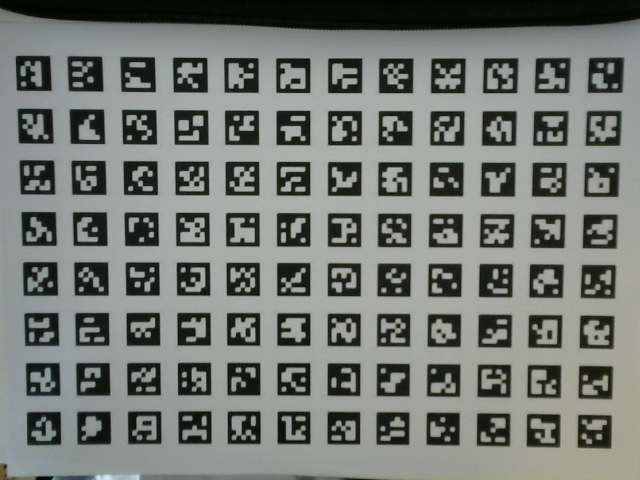
\includegraphics[width=\textwidth]{../Figures/camera_calibration/1.png}
        \caption{}
        \label{fig:gazebo_gps2vision_board}
    \end{subfigure}
     \hspace{0.2em}
    \begin{subfigure}[t]{.22\textwidth}
        \centering
        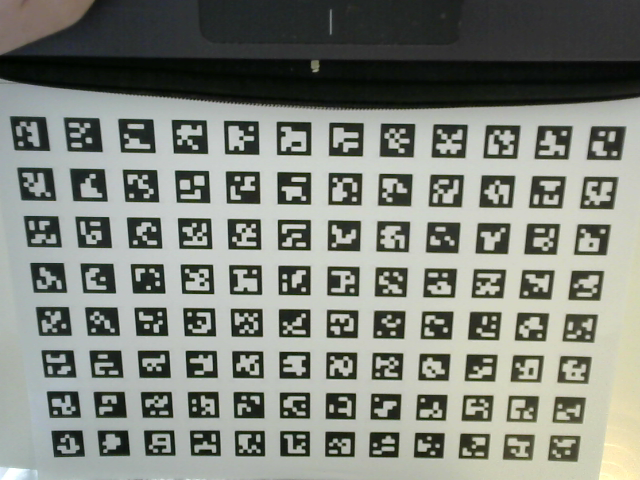
\includegraphics[width=\textwidth]{../Figures//camera_calibration/3.png}
        \caption{}
        \label{fig:gazebo_landing_board_one}
    \end{subfigure}
     \hspace{0.2em}
    \begin{subfigure}[t]{.22\textwidth}
        \centering
        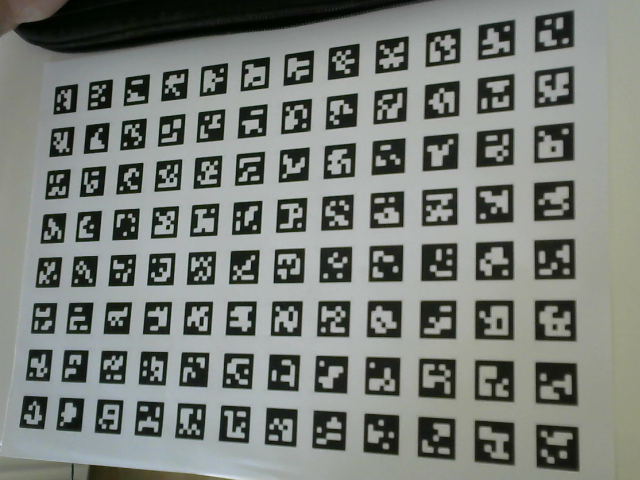
\includegraphics[width=\textwidth]{../Figures//camera_calibration/4.png}
        \caption{}
        \label{fig:gazebo_landing_board_two}
    \end{subfigure}
         \hspace{0.2em}
    \begin{subfigure}[t]{.22\textwidth}
        \centering
        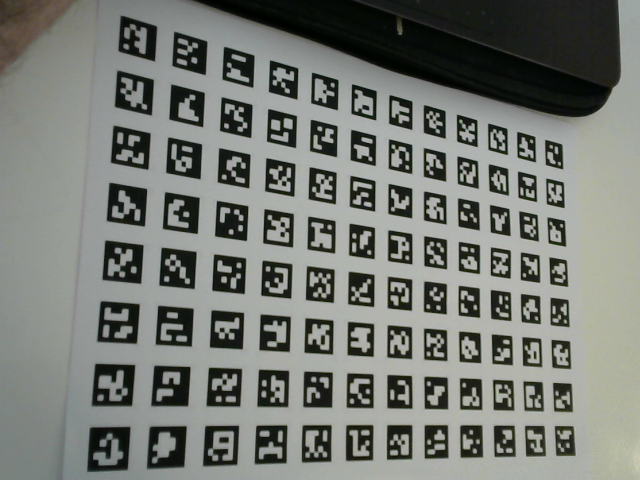
\includegraphics[width=\textwidth]{../Figures/camera_calibration/5.png}
        \caption{}
        \label{fig:gazebo_landing_board_three}
    \end{subfigure}
    \caption{Illustration }  
    \label{fig:gazebo_aruco_marker_boards}
\end{figure}    


\subsection{Sensor fusion}
\label{sec:sensor_fusion}
Chances are that ArUco markers placed on the ground will not be visible at all times. This can be due to changes in light conditions and dirt on or wear of the markers. This could be fatal, because the drone in offboard control will relie on constant updates from the pose of ArUco markers when flying indoors. To mitigate this situation sensor fusion will be implemented. 

This section deals with the implementation of sensor fusion for pose estimation. Section \ref{sec:ukf} is about the theory behind the Unscented Kalman filter (UKF) and why using this would be beneficial in regards to other methods e.g. the extended Kalman filter (EKF). Section \ref{sec:ukf_implementation} deals with the implementation of the UKF.   

\subsubsection{Unscented Kalman Filter}
\label{sec:ukf}

The Kalman Filter (KF) requires linear models. However, these models are rarely seen in reality and especially not in the dynamics of a Aquacopter. A way to accommodate for this problem could be to approximate the linear model by linearization using an EKF. The basic idea behind this approach is to use the mean of a non-linear Gaussian function and linearize at this single point through Taylor expansion. However, because the EKF only offers \textit{first order} approximations of the optimal terms based on a liniarization for the non linear system of the estimated state destribution of a Gaussion Random Variable (GRV), large errors can occur if functions turn out to be \textit{very} nonlinear. Furthermore, calculations of the Jacobaion are needed which can intruduce errrors if not performed correcly. Becuase of these limitations, this method is considered sub-optimal.  

\begin{figure}[H]
	\centering
	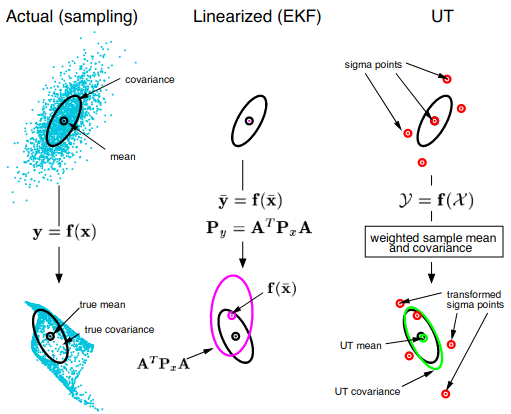
\includegraphics[height=7.0cm]{../Figures/ukf.png}
	\caption{Illustration of the uncented transformation (UT) and how the use of this method in the UKF performas better than EKF in regard to better mean and covariance estimation \cite{UnscentedKalmanFilter}} \label{fig:ut}
\end{figure}

Another method called UKF takes these considerations into account. The state distribution is still represented using a GRV. However, now a number of sample points around the mean called \textit{sigma points} are chosen which better captures the true mean and covariance of the GRV of the non-linear system using the unscented transformation (UT). An illustration of the superiority of using the UT instead of a first-order linearization in the EKF can be seen in Figure \ref{fig:ut}. For Gaussian functions, the use of the UT results in approximations which are accurate to the third order and at least second order for non Gaussian functions for all nonlinearities. For a more in-depth explanation of the UKF, the paper \cite{UnscentedKalmanFilter} is recommended.  

Because of the discussed optimizations in regard to the EKF, the UKF will be used in the implementation of sensor fusion for estimating the pose of the drone. 

\subsubsection{UKF implementation}
\label{sec:ukf_implementation}

Because the appropriate choose for parameters of sigma points may give performance improvements, these have been chosen based on a discussion of the UKF in \cite[p.~354]{KalmanAndBayesianFiltersInPython}. Three initial parameters have to be chosen namely $\alpha$, $\beta$ and $k$. $\alpha$ determines the amount of spread of the sigma points from the mean of $\bar{x}$ which is chosen to be 0.04, $\beta$ incorporates prior knowledge of the distribution of $x$ which is set to 2 and $\mathcal{k}$ is defined as a secondary scaling parameter set to 15. The equations for the calculations of \textit{sigma points} can be seen in Equation \ref{eq:update_zero_sigma_point}, \ref{eq:update_ith_sigma_point_plus} and \ref{eq:update_ith_sigma_point_minus} in Pseudocode \textit{UKF calculate sigma points} with associated weights seen in Equation \ref{eq:init_weight_zero_mean}, \ref{eq:init_weight_zero_covariance}, \ref{eq:init_weight_zero_mean} and \ref{eq:init_weight_zero_covariance}. To calculate the weights, a scaling parameter $\lambda = \alpha^2(L+k)-L$ where $L$ is the number of states in the system is used. The superscipt $(m)$ and $(c)$ in the weights defines the mean and covariance of the weights respectively. The initialization of the UKF can be seen in Pseudocode \textit{UKF initialization}. Besides the already defined parameters, the process noise matrix $Q$ and measurements noise matrix $R$ must be set. These can be seen in Equation \ref{eq:process_noise} and \ref{eq:measurement_noise} respectively. Both have been set as diagonal matrices with noise in position x, y and z, noise in velocity in x and y, noise in euler angles in roll, pitch and yaw and noise in euler angle rates in roll, pitch and yaw starting from $(0,0)$ to $(12,12)$ for both matrix $Q$ and $R$. However, with two additional measurement noise parameters in $R$ for altimeter height in $(13,13)$ and altimeter error in $(14,14)$. This results in twelve states in the system to track.

\setcounter{MaxMatrixCols}{13}
\begin{equation}
\small
Q = 
\begin{bmatrix}
0.5 & 0 & 0 & 0 & 0 & 0 & 0 & 0 & 0 & 0\\
0 & 0.5 & 0 & 0 & 0 & 0 & 0 & 0 & 0 & 0\\
0 & 0 & 0.5 & 0 & 0 & 0 & 0 & 0 & 0 & 0\\
0 & 0 & 0 & 0.5 & 0 & 0 & 0 & 0 & 0 & 0\\
0 & 0 & 0 & 0 & 0.5 & 0 & 0 & 0 & 0 & 0\\
0 & 0 & 0 & 0 & 0 & 0.5 & 0 & 0 & 0 & 0\\
0 & 0 & 0 & 0 & 0 & 0 & 0.5 & 0 & 0 & 0\\
0 & 0 & 0 & 0 & 0 & 0 & 0 & 0.5 & 0 & 0\\
0 & 0 & 0 & 0 & 0 & 0 & 0 & 0 & 0.5 & 0\\
0 & 0 & 0 & 0 & 0 & 0 & 0 & 0 & 0 & 3.0
\end{bmatrix}
\label{eq:process_noise}
\end{equation}

\begin{equation}
\small
R = 
\begin{bmatrix}
0.011& 0 & 0 & 0 & 0 & 0 & 0 & 0 & 0 & 0 & 0 & 0 & 0\\
0 & 0.011& 0 & 0 & 0 & 0 & 0 & 0 & 0 & 0 & 0 & 0 & 0\\
0 & 0 & 0.011& 0 & 0 & 0 & 0 & 0 & 0 & 0 & 0 & 0 & 0\\
0 & 0 & 0 & 0.300 & 0 & 0 & 0 & 0 & 0 & 0 & 0 & 0 & 0\\
0 & 0 & 0 & 0 & 0.300 & 0 & 0 & 0 & 0 & 0 & 0 & 0 & 0\\
0 & 0 & 0 & 0 & 0 & 0.005 & 0 & 0 & 0 & 0 & 0 & 0 & 0\\
0 & 0 & 0 & 0 & 0 & 0 & 0.005 & 0 & 0 & 0 & 0 & 0 & 0\\
0 & 0 & 0 & 0 & 0 & 0 & 0 & 0.005 & 0 & 0 & 0 & 0 & 0\\
0 & 0 & 0 & 0 & 0 & 0 & 0 & 0 & 0.030 & 0 & 0 & 0 & 0\\
0 & 0 & 0 & 0 & 0 & 0 & 0 & 0 & 0 & 0.030 & 0 & 0 & 0\\
0 & 0 & 0 & 0 & 0 & 0 & 0 & 0 & 0 & 0 & 0.030 & 0 & 0\\
0 & 0 & 0 & 0 & 0 & 0 & 0 & 0 & 0 & 0 & 0 & 0.500 & 0\\
0 & 0 & 0 & 0 & 0 & 0 & 0 & 0 & 0 & 0 & 0 & 0 & 0.500
\end{bmatrix}
\label{eq:measurement_noise}
\end{equation}

\begin{Pseudo}{UKF initialization}{}
\begin{Indentation}
	\item Given scalar values for initialization of $\alpha$, $\beta$, $k$ and $L$
	\item $\alpha$ \( \leftarrow Chosen\, alpha \)
	\item $\beta$ \( \leftarrow Chosen\, beta \)
	\item $k$ \( \leftarrow Chosen\, k \)
	\item $L$ \( \leftarrow Number\, of\, states \)
	\item Given vectors of size $L$ for $x$ with a matrices of size $L \times L$ for $Q$ and  $P$ 
	\item $x$ \( \leftarrow Initial\, state\)
	\item $Q$ \( \leftarrow Process\, noise \)
	\item $P$ \( \leftarrow Initial\, covariance \)
	\item Initialize function which predicts next state
	\item $iterate$ \( \leftarrow iterateFunction(x,dt) \)
	\item Initialize weights for associated sigma points 
	\item $W^{(m)}_0$ \( \leftarrow \frac{\lambda}{L+\lambda} \)  \qquad \refstepcounter{equation}(\theequation)\label{eq:init_weight_zero_mean}
	\item $W^{(c)}_0$ \( \leftarrow \frac{\lambda}{L+\lambda} + (1-\alpha^2 +\beta)	\)  \qquad \refstepcounter{equation}(\theequation)\label{eq:init_weight_zero_covariance}

    \item \textbf{for} $i$ \(\leftarrow 1\, to\, 2L\) \textbf{do}
        \begin{Indentation}
            \item $W^{(m)}_i$ \(\leftarrow \frac{1}{2(L+\lambda)} \) \qquad \refstepcounter{equation}(\theequation)\label{eq:init_weight_ith_mean}
            \item $W^{(c)}_i$ \(\leftarrow \frac{1}{2(L+\lambda)} \) \qquad \refstepcounter{equation}(\theequation)\label{eq:init_weight_ith_covariance} \vspace{-5pt}
    \end{Indentation}
\end{Indentation}
\end{Pseudo}

Because the measurement updates in the pose comes from the estimated ArUco marker pose, the noise in position and orientation have been decided based on the worst STD in Section \ref{sec:hold_pose_using_aruco_pose_estimation} where the error in the estimated ArUco pose were based on a comparison to that of the ground truth. The worst STD where found to be 0.011 meters and 0.005 radians for the position and orientation respectively. Due to the fact that the sensor noise from the accelerometer and gyro are quite noise, these parameters have been chosen to be higher than that of the pose to put more trust on ArUco marker updates. The STD has therefore been set to 0.3 $\frac{m}{s}$ and 0.03 $\frac{r}{s}$ for the velocities in x and y and angular rates from the accelerometer and gyro respectively. Lastly, the noise for height estimates and associated errors between the height estimate and ArUco marker position in z have been set to 0.5 meters because the updates from the barometer tends to be quite noisy as well. The parameters for the process noise where found appropriate by trial and error.

In Pseudocode \textit{UKF initialization}, one may notice the initialization of the $iterateFunction(x,dt)$. This function defines the update of the state in the prediction step of the UKF algorithm. This function can be seen in Pseudocode \textit{UKF iterate function}.           

\begin{Pseudo}{UKF iterate function}{}
\begin{Indentation}
	\item $x$ \( \leftarrow State \)
	\item $dt$ \( \leftarrow\, Time\, since\, last\, update \)
	\item $x^{new}_0$ \(\leftarrow x_0 + 0.6 \cdot x_3 \cdot dt\) \qquad ($Position\, in\, x$)
	\item $x^{new}_1$ \(\leftarrow x_1 + 0.6 \cdot x_4 \cdot dt\) \qquad ($Position\, in\, y$)
	\item $x^{new}_2$ \(\leftarrow x_2\) \qquad ($Position\, in\, z$)
	\item $x^{new}_3$ \(\leftarrow x_3\) \qquad ($Velocity\, in\, x$)
	\item $x^{new}_4$ \(\leftarrow x_4\)\qquad ($Velocity\, in\, y$)
	\item $x^{new}_5$ \(\leftarrow x_5 + x_8 \cdot dt\) \qquad ($Angle\, in\, Roll$)
	\item $x^{new}_6$ \(\leftarrow x_6 + x_{9} \cdot dt\) \qquad ($Angle\, in\, Pitch$)
	\item $x^{new}_7$ \(\leftarrow x_7 + x_{10} \cdot dt\) \qquad ($Angle\, in\, Yaw$)
	\item $x^{new}_8$ \(\leftarrow x_8 \) \qquad ($Velocity\, in\, Roll$)
	\item $x^{new}_9$ \(\leftarrow x_9 \) \qquad ($Velocity\, in\, Pitch$)
	\item $x^{new}_{10}$ \(\leftarrow x_{10} \) \qquad ($Velocity\, in\, Yaw$)
	\item $x^{new}_{11}$ \(\leftarrow x_{11} \) \qquad ($Error\, in\, altimeter$)
	\item $return$ $x_{new}$	
\end{Indentation}
\label{pse:ukf_iterate_function}
\end{Pseudo}

Here it may be noticed that the values from the accelerometer $x_3$ and $x_4$ are directly passed to the updates in position for x and y with only a single integration. To be completely mathematical correct, these values should have to be put through a double integration from where one goes from acceleration to velocity and velocity to position. The reason for doing this is because of the accumulation in error when integrating twice. To mitigate this issue, only a single integration is used with multiplication of a constant with a value of 0.6 which is found appropriate. Hence, the values from the accelerometer is interpreted as a velocity which reduces error and let go of the need for implementation of \textit{movement end checking} \cite[p.~6]{ImplementingPositioningAlgorithmsUsingAccelerometers}. The need for this implementation would have been likely because the area under the integration curve due rarely align when the acceleration \textit{flips} the opposite way until reaches zero. This may create an accumulated velocity even thought the vehicle is not moving. This approach is only possible because the implementation of sensor fusion is to be used in indoor environments where the drone is not exposed to wind. Otherwise the integration of the values from the accelerometer when the drone having an angle in pitch or roll due to wind, would lead to errors in the position estimation.

In regard to the updates of the altitude of the drone when no new ArUco marker pose is available, a barometer is used. Because barometers uses atmospheric pressure to calculate the altitude, errors in height can occur when pressure or temperature changes. To take into account these scenarios, the error between the altitude estimated from the ArUco marker pose and that of the barometer is calculated every time new pose estimates from ArUco markers are available. This estimated error is then subtracted from the height estimate from the barometer when the barometer is used to update the altitude of the drone. 

\begin{Pseudo}{UKF calculate sigma points}{}
\begin{Indentation}
	\item $\mathcal{X_0}$  \(\leftarrow \bar{x}\) \qquad \refstepcounter{equation}(\theequation)\label{eq:update_zero_sigma_point}
	\item \textbf{for} $i$ \(\leftarrow 1\, to\, L\) \textbf{do}
        \begin{Indentation}
            \item $\mathcal{X_i}$ \(\leftarrow \bar{x} + \left(\sqrt{(L+\lambda})P_i\right)\) \qquad \refstepcounter{equation}(\theequation)\label{eq:update_ith_sigma_point_plus}
         \end{Indentation}
            
    \item \textbf{for} $i$ \(\leftarrow L+1\, to\, 2L\) \textbf{do}
        \begin{Indentation}
            \item $\mathcal{X_i}$ \(\leftarrow \bar{x} - \left(\sqrt{(L+\lambda})P_i\right)\) \qquad \refstepcounter{equation}(\theequation)\label{eq:update_ith_sigma_point_minus}
    	\end{Indentation}
    	\item $return\, \mathcal{X}$
\end{Indentation}
\end{Pseudo}

\begin{Pseudo}{UKF prediction update}{}
\begin{Indentation}

	\item Prediction step for sigma points  
	\item \textbf{for} $i$ \(\leftarrow 0\, to\, 2L\) \textbf{do}
        \begin{Indentation}
            \item $\mathcal{X}_i$ \(\leftarrow irerateFunction(\mathcal{X}_i,dt) \) \qquad \refstepcounter{equation}(\theequation)\label{eq:update_predict_sigma_points}
        \end{Indentation}
    
    \item Prediction step for state
	\item \textbf{for} $i$ \(\leftarrow 0\, to\, L\) \textbf{do}
        \begin{Indentation}
        	\item \textbf{for} $j$ \(\leftarrow 0\, to\, 2L\) \textbf{do}
        		\begin{Indentation}
            		\item $x_i$ \(\leftarrow  x_i +  W^{m}_j \cdot \mathcal{X}_{ij} \)  \qquad \refstepcounter{equation}(\theequation)\label{eq:update_predict_state}
         		\end{Indentation}
         \end{Indentation}	
         
    \item Prediction step for covariance matrix
	\item \textbf{for} $i$ \(\leftarrow 0\, to\, 2L\) \textbf{do}
        \begin{Indentation}
            \item $P$ \(\leftarrow P + W^{c}_i \cdot (\mathcal{X}_i - x_i)(\mathcal{X}_i - x_i)^T \) \qquad \refstepcounter{equation}(\theequation)\label{eq:update_predict_covariance}
        \end{Indentation}
    \item $P$ \(\leftarrow P + Q \cdot dt \)
\end{Indentation}
\end{Pseudo}

\begin{Pseudo}{UKF measurement update}{}
\begin{Indentation}

	\item $\mathcal{Y}$ \(\leftarrow Sigma\, points\, for\, measurements \)
	\item $\mathbf{y}$ \(\leftarrow Measurements \)
	\item $\mathbf{R}$ \(\leftarrow Measurement\, noise \)
	\item Covariance of measurements  
	\item \textbf{for} $i$ \(\leftarrow 0\, to\, 2L\) \textbf{do}
        \begin{Indentation}
            \item $P_{yy}$ \(\leftarrow P_{yy} + W^{c}_i \cdot (\mathcal{Y}_i - y_i)(\mathcal{Y}_i - y_i)^T \) \qquad \refstepcounter{equation}(\theequation)\label{eq:update_measurement_covariance_of_measurements}
        \end{Indentation}
     \item  $P_{yy}$ \(\leftarrow  P_{yy} + R\)
        
    \item Covariance of measurement with states 
	\item \textbf{for} $i$ \(\leftarrow 0\, to\, 2L\) \textbf{do}
        \begin{Indentation}
            \item $P_{xy}$ \(\leftarrow P_{xy} + W^{c}_i \cdot (\mathcal{X}_i - x_i)(\mathcal{Y}_i - y_i)^T \)  \qquad \refstepcounter{equation}(\theequation)\label{eq:update_measurement_covariance_of_measurements_with_states}
        \end{Indentation}
        
    \item Calculate Kalman gain  
    \item $\mathcal{K}$ \(\leftarrow P_{xy} \cdot P^{-1}_{yy} \)  \qquad \refstepcounter{equation}(\theequation)\label{eq:update_measurement_kalman_gain}
     
    \item Update state  
    \item $x$ \(\leftarrow x + \mathcal{K}(y- \bar{y}) \)  \qquad \refstepcounter{equation}(\theequation)\label{eq:update_measurement_state}
    
    \item Update covariance   
    \item $P$ \(\leftarrow P - \mathcal{K} P_{yy} \mathcal{K}^T \)  \qquad \refstepcounter{equation}(\theequation)\label{eq:update_measurement_covariance}
    
    \item Update sigma points   
    \item $\mathcal{X}$ \(\leftarrow Calculate\, sigma\, points\)  
\end{Indentation}
\end{Pseudo}

Pseudocode code for the prediction and measurement update can be seen in \textit{UKF prediction update} and \textit{UKF measurement update}. In the prediction step, the sigma points and state will be updated along with covariance. In the measurement update, the state to be updated is used, where the Kalman gain is calculated based on covariance of the measurement and measurement with states. This Kalman gain is then used to update the state and covariance of the system. 

In regard to the sensor noise in the accelerometer and gyro, they are found by taking the mean of the first 10 seconds of measurements when the drone is initiated and then subtracting this value from new measurement updates. These measurements will then have to be aligned with the ArUco marker pose estimation, which is done by multiplying the data from the accelerometer and gyro by a rotation matrix from the current IMU sensor placement on the drone. Moreover, the barometer error will be estimated as soon as new ArUco pose estimates are available to the system.  

\subsection{Companion computer}
\label{sec:companion_computer}

\subsubsection{Operating system}

\todo{Why use Ubuntu 18.04 instead of the official raspian operating system for raspberry pi?}

For onboard computing a Raspberry Pi 4 is used with an Ubuntu 18.04.5 LTS (Bionic Beaver) 64-bit server operating system. The 64-bit version is used because the Raspberry Pi 4 is build on a 64-bit architecture and the server edition is chosen to minimize overhead because the graphical user interface (GUI) is not needed as the interface used for communicating to the Raspberry Pi will be through ssh from the terminal. The mentioned operating system can be fetched from the official Ubuntu website \cite{ubuntuImage}. The Raspberry Pi 4 gives a number of possibles options in regard to system boot, but in this case an SD card will be used. Now  \href{https://www.balena.io/etcher/}{etcher} is used to flash the Ubuntu 18.04.5 image to the SD card which offers a secure way for image flashing. 

\subsubsection{Wireless communication}
To enable ssh for a wired communication between laptop and Raspberry Pi, the following lines of code from the terminal are executed as seen in Listing \ref{lst:enable_ssh}.      

\begin{lstlisting}[frame=none,caption={How to enable ssh communication by making a file called \textit{ssh} to system-boot of the sd card}, label=lst:enable_ssh]
#Change directory to system-boot
$ cd /media/<user>/system-boot/
#Make a file called ssh
$ touch ssh
\end{lstlisting}

To access the Raspberry Pi from the terminal, the correct IP-address of the Raspberry Pi must be known. This can be done using the protocol \textit{nmap} which searches for all possible IP-addresses in a defined sub-network in the local network. This is done using Listing \ref{lst:ip_address_ssh}. When the correct IP-address is found, an ssh connection can be established. 

\begin{lstlisting}[frame=none, caption={Find the IP-address of the Raspberry Pi for \textit{ssh} communication},label=lst:ip_address_ssh]
#Find the IP-address of eth0 (Raspberry Pi) 
$ ifconfig	
#Find hosts in specific address range 
$ nmap -sn <ip-address-eth0>/24
#SSH into Raspberry Pi 
$ ssh ubuntu$<ip-address-raspberry-pi>
\end{lstlisting}

Because the goal is to have a wireless connection to the Raspberry Pi from an access point using WiFi, the net-plan has to be configured from \textit{/etc}  in the system configuration files of the Raspberry Pi. The file to be updated can be seen in Listing \ref{lst:wireless_connection_setup_file}. Here the SSID (name of WiFi network) must be configured along with the password of the WiFi network. 

\begin{lstlisting}[frame=none, caption={File to configure to enable wireless connection},label=lst:wireless_connection_setup_file]
#File /etc/netplan/50-cloud-init.yaml
network:
    ethernets:
        eth0:
            dhcp4: true
            optional: true
    version: 2
    wifis:
        wlan0:
            optional: true
            access-points:
                "<YourSSID>":
                    password: "<YourPassword>"
            dhcp4: true

\end{lstlisting}

Using \href{https://www.vim.org/}{vim} or another text editor, the mentioned file can be updated using Listing \ref{lst:wireless_connection_setup} from the established wired ssh connection.  

\begin{lstlisting}[frame=none, caption={Create an access point from a wireless connection by configuring netplan},label=lst:wireless_connection_setup]
#Configure access point changing the wlan0 settings
$ sudo vim /ect/netplan/50-cloud-init.yaml
#Apply settings  
$ sudo netplan apply
\end{lstlisting}

Now the outgoing IP-address through WiFi from the Raspberry Pi can be found. This IP-address can now be used to \textit{ssh} into Raspberry Pi if both the Laptop and Raspberry Pi are connected to the same WiFi network.

\end{document}